% compile with lualatex and biber
% run makeglossaries on command line if glossary changed

\documentclass[
    a4paper,
    12pt,
    twoside,
    BCOR=12mm,
    parskip=half,
    chapterprefix,
    numbers=noenddot,
    bibliography=totoc
]{scrbook}

\usepackage{scrhack}

\usepackage[T1]{fontenc}
\usepackage[log-declarations=false]{xparse} % http://tex.stackexchange.com/questions/46683
\usepackage[svgnames]{xcolor}

\usepackage{amsmath}
\usepackage{amsthm}
\usepackage{thmtools} % for custom 'qed' symbol outside proofs
\usepackage{amssymb}
\usepackage{mathtools} % for math versions of \llap, \rlap etc.

\usepackage[framemethod=TikZ]{mdframed}
\colorlet{shadecolor}{gray!10}

\usepackage{bm} % bold math: \bm{..}
\newcommand{\bftt}[1]{\textbf{\texttt{#1}}}	% typesets as text in math mode

%\newcommand{\ts}[1]{\bftt{#1}} % ts = terminal symbol
% vphantom für trees http://tex.stackexchange.com/a/100859/6255
\newcommand{\ts}[1]{\bftt{#1}\protect\vphantom{\bftt{(}}} 

\allowdisplaybreaks[1] % split long equations on page breaks

% fix spacing for \left..\right
% http://tex.stackexchange.com/questions/2607/spacing-around-left-and-right
\let\originalleft\left
\let\originalright\right
\renewcommand{\left}{\mathopen{}\mathclose\bgroup\originalleft}
\renewcommand{\right}{\aftergroup\egroup\originalright}
%\usepackage{mleftright}

\theoremstyle{plain}
%\newtheorem{theorem}{Theorem}
\newtheorem{lemma}{Lemma}
\newtheorem{proposition}{Proposition}
\newtheorem*{corollary}{Corollary}

\declaretheoremstyle[
	spaceabove=10pt,
	notefont=\normalfont,
	headpunct={\normalfont:},
	bodyfont=\normalfont,
	postheadspace=\newline,
	qed=\ensuremath{\triangleleft}
]{mydefinition}

\declaretheoremstyle[
	spaceabove=0pt,
	spacebelow=0pt,
	notefont=\normalfont,
	headpunct={\normalfont:},
	bodyfont=\normalfont,
	postheadspace=\newline
]{myexample}

\declaretheoremstyle[
	spaceabove=10pt,
	notefont=\normalfont,
	headpunct={\normalfont:},
	bodyfont=\normalfont\itshape,
	postheadspace=\newline,
	qed=\ensuremath{\triangleleft}
]{mytheorem}

\declaretheoremstyle[
	numbered=no,
	spaceabove=6pt,
	headfont=\normalfont\itshape,
	notefont=\normalfont,
	headpunct={\normalfont:},
	bodyfont=\normalfont,
	qed=\ensuremath{\triangleleft}
]{myremark}

\renewcommand\thmcontinues[1]{Continued}

\declaretheorem[name=Definition,style=mydefinition]{definition}

\declaretheorem[name=Example,style=myexample,
	mdframed={
		hidealllines=true,leftline=true,bottomline=true,roundcorner=5pt,
    innertopmargin=0pt,
		rightmargin=0pt,innerrightmargin=0pt,
		innerlinewidth=0pt,middlelinewidth=0pt,
		outerlinecolor=shadecolor,outerlinewidth=3pt,
    backgroundcolor=none,
		skipabove=\topskip,skipbelow=\topskip,
		}
	]{example}

\declaretheorem[name=Theorem,style=mytheorem]{theorem}

\declaretheorem[name=Remark,style=myremark]{remark}
\declaretheorem[name=Note,style=myremark]{note}

%\newcommand*{\op}[1]{\operatorname{#1}}
\newcommand*{\op}[1]{\mathrm{#1}}

%\usepackage{stmaryrd} % for double brackets
\usepackage{textcomp} % for double brackets
%workaround until stmaryrd works
\newcommand*{\llbracket}{\text{\textlbrackdbl}}
\newcommand*{\rrbracket}{\text{\textrbrackdbl}}

\newcommand\concat{\ensuremath{\mathbin{+\mkern-5mu+}}}
\usepackage{fontspec}
\usepackage{mathpazo} % non-fancy math font for Pagella/Palatino

\defaultfontfeatures{Ligatures=TeX}

% use microtype, see http://tex.stackexchange.com/a/42539/6255
\pdfprotrudechars=2
\pdfadjustspacing=2
\newfontfeature{Microtype}{protrusion=default;expansion=default;}

% see http://tex.stackexchange.com/questions/48159
\directlua{fonts.protrusions.setups.default.factor=0.5} % default: 1
\directlua{fonts.expansions.setups.default.stretch=1.5} % default: 2

\setmainfont[Microtype]{TeX Gyre Pagella}
\setsansfont{TeX Gyre Heros}

\frenchspacing

\setkomafont{caption}{\small}
\setkomafont{captionlabel}{\usekomafont{caption}}
\usepackage{fancyvrb}

\usepackage{listings}
\usepackage{caption}

\lstset{
  basicstyle=\small\ttfamily,
  breaklines=true,
  numbers=left,
  numberblanklines=false,
  numberstyle=\tiny,
  captionpos=t,
  language=Haskell
}

\DeclareCaptionFont{white}{\color{white}}
\DeclareCaptionFormat{listing}{\colorbox{gray}{\parbox{\textwidth-6.8pt}{#1#2#3}}}
\captionsetup[lstlisting]{format=listing,labelfont=white,textfont=white}

\usepackage{enumitem} % http://tex.stackexchange.com/questions/10684/vertical-space-in-lists

\usepackage{quoting}
\usepackage[threshold=2]{csquotes}
\SetBlockEnvironment{quoting}

\usepackage{graphicx}
\usepackage{tikz}
\usetikzlibrary{positioning,fit,chains,calc}

\usepackage{gnuplot-lua-tikz}

\makeatletter
% tikz-qtree workaround http://tex.stackexchange.com/a/66927/6255
\let\orig@tikz@edge@to@parent@path=\tikz@edge@to@parent@path
\tikzset{
  original tree type/.code={%
    \let\tikz@edge@to@parent@path=\orig@tikz@edge@to@parent@path
  }
}
\makeatother

\tikzset{
	math mode/.style={
		execute at begin node=$,
		execute at end node=$
	}
}

\tikzset{
	grammar rule tree/.style={
	  math mode,
		baseline={([yshift=-2.3ex]current bounding box.north)}
	}
}

% see http://tex.stackexchange.com/a/88548/6255
\newbox\collectbox
\tikzset{
    raise text/.style={
        execute at begin node={\setbox\collectbox=\hbox\bgroup},
        execute at end node={%
            \egroup%
            \phantom{\copy\collectbox}%
            \kern-\wd\collectbox%
            \smash{\raisebox{#1}{\box\collectbox}}}
    }
}

% styles for RNA grammar diagrams
\tikzset{
	rna grammar rule/.style={
		remember picture, % needed when reverse clipping is used
		start chain,
		node distance=0.25,
		every join/.style={thick},
		basepair edge/.style={
			ultra thick,
			out=50,in=130
		},
		font=\footnotesize
	},
	char/.style={
		on chain,
		inner sep=0pt
	},
	nonterminal/.style={
		rectangle,
		draw,
		on chain,
		minimum width=50pt,
		minimum height=14pt,
	},
	phantom rectangle/.style={
		on chain,
		minimum size=14pt,
	},
	terminal/.style={
		char,
		draw,
		circle,
		minimum size=14pt,
		text height=1.5ex,text depth=.25ex % adjust baselines
	},
	empty word/.style={
		rectangle,
		dashed,
		draw,
		on chain,
		minimum size=14pt
	},
	base/.style={
		circle,
		draw,
		fill,		
		on chain,
		minimum size=14pt
	},
	derive sign/.style={
		char,
		inner xsep=5pt,
		font=\Huge,
		execute at begin node=\raisebox{-0.4cm}{$\rightarrow$}
	},
	or sign/.style={
		char,
		font=\Huge,
		execute at begin node=|
	}
}

% styles for RNA secondary structures
\tikzset{
	rna secondary structure/.style={
		node distance=0.2,
		font=\footnotesize,
		every join/.style={thick},
		basepair edge/.style={ultra thick},
		natural/.style={
			every node/.style={terminal,join},
			start chain
		},
		linear/.style={
			every node/.style={terminal,join},
			start chain,
			basepair edge/.style={
				ultra thick,
				out=90,in=90
			}
		},
		circular/.style 2 args={% number of nodes, radius
			every node/.style={terminal,join},
			start chain=placed {at=(270-\tikzchaincount*360/##1+180/##1:##2)}
		},
		filled bases/.style={
			every node/.style={base,join},
		},
		count bases/.style={
			execute at end node=\tikzchaincount
		},
		dot bracket/.style={% useful for aligning under linear style
			every node/.style={% same as terminal, but without ``draw'' and bigger font
				char,
				circle,
				font=\normalsize\ttfamily,
				minimum size=14pt,
				text height=1.5ex,text depth=.25ex % adjust baselines
			},
			start chain
		},
		dot bracket primary/.style={% useful for aligning under linear style
			dot bracket,
			every node/.style={% same as terminal, but without ``draw'' and bigger font
				char,
				circle,
				font=\footnotesize,
				minimum size=14pt,
				text height=1.5ex,text depth=.25ex % adjust baselines
			},
		}
	}
}

% two dimensional nonterminal
% the phantom nodes should be rectangles (to access their anchors)
\newcommand*{\nonterminaltwo}[4][0.0]{% looseness adjustment (optional),1st node, 2nd node, label text
	\pgfmathsetmacro{\loosea}{0.85+(#1)}
	\pgfmathsetmacro{\looseb}{1.0+(#1)}
	\draw[save path=\myclippath]
				(#2.south east) to [in=90, out=90, looseness=\loosea] node[above=-1pt]{#4} (#3.south west)
				-- (#3.south east)
				to [in=90, out=90, looseness=\looseb] (#2.south west) -- cycle;
	\reverseclip{\myclippath}
}

\tikzset{
  reverseclip/.style={
    clip even odd rule,
    insert path={(current page.north east) --
      (current page.south east) --
      (current page.south west) --
      (current page.north west) --
      (current page.north east)}
  },
  clip even odd rule/.code={\pgfseteorule}
}

\newcommand*{\reverseclip}[1]{
  \begin{pgfinterruptboundingbox}
      \clip[reverseclip] \againpath #1;
  \end{pgfinterruptboundingbox}
}

% http://tex.stackexchange.com/a/28537/6255
% usage: \draw[red] \convexpath{a,b,c,d}{1cm};
% ACHTUNG: nodes müssen im uhrzeigersinn angegeben werden
\newcommand{\convexpath}[2]{
  [   
  create hullcoords/.code={
    \global\edef\namelist{#1}
    \foreach [count=\counter] \nodename in \namelist {
      \global\edef\numberofnodes{\counter}
      \coordinate (hullcoord\counter) at (\nodename);
    }
    \coordinate (hullcoord0) at (hullcoord\numberofnodes);
    \pgfmathtruncatemacro\lastnumber{\numberofnodes+1}
    \coordinate (hullcoord\lastnumber) at (hullcoord1);
  },
  create hullcoords
  ]
  ($(hullcoord1)!#2!-90:(hullcoord0)$)
  \foreach [
  evaluate=\currentnode as \previousnode using \currentnode-1,
  evaluate=\currentnode as \nextnode using \currentnode+1
  ] \currentnode in {1,...,\numberofnodes} {
    let \p1 = ($(hullcoord\currentnode) - (hullcoord\previousnode)$),
    \n1 = {atan2(\x1,\y1) + 90},
    \p2 = ($(hullcoord\nextnode) - (hullcoord\currentnode)$),
    \n2 = {atan2(\x2,\y2) + 90},
    \n{delta} = {Mod(\n2-\n1,360) - 360}
    in 
    {arc [start angle=\n1, delta angle=\n{delta}, radius=#2]}
    -- ($(hullcoord\nextnode)!#2!-90:(hullcoord\currentnode)$) 
  }
}

%\newcommand*{\arcthickness}{1}
%\newcommand*{\myarc}[4]{ % x,y,radius,text  
%
   %node is positioned by splitting the arc in two parts (workaround until new pgf is released)
   %see http://tex.stackexchange.com/a/76369/6255
  %\draw[thick,save path=\arcclippath] 
              %(#1,#2) arc (180:90:#3)
              %node[below=-1.5pt] {\tiny #4}
              %arc (90:0:#3)
              %-- ++(-\arcthickness,0) arc (0:180:#3-\arcthickness) -- cycle;
	%\reverseclip{\arcclippath}
%}
%
%\newcommand{\secstruc}[3]{ % x,y,radius
	%\draw [thick] (#1,#2) -- ++(#3*2,0);
	%\draw [thick,dash pattern=on 2pt off 1pt] (#1+2*#3,#2) arc (0:180:#3);
%}

%\begin{tikzpicture}[remember picture,x=0.3cm,y=0.3cm]
	%
	%\myarc{4.8}{0}{4.1}{Hs}
	%\myarc{2.4}{0}{4.1}{Hs}
	%\myarc{0}{0}{4.1}{G}
	%\secstruc{1.2}{0}{0.5}
	%\secstruc{3.6}{0}{0.5}
	%\secstruc{6}{0}{0.5}
	%\secstruc{10.8}{0}{0.5}
	%
%\end{tikzpicture}


% need matrix functionality for that
%\begin{tikzpicture}[rna secondary structure]
	%\begin{scope}[natural]
		%\node[continue chain=going above] {C};
		%\node {A};
		%\node {A};
		%\node {U};
		%\node {U};
		%\node {U};
		%\node {U};
		%\node[yshift=19pt] {C};
		%\node[continue chain=going right,xshift=20pt] {U};
		%\node[continue chain=going below] {G};
		%\node[] {A};
		%\node[join=with chain-6 by {basepair edge}] {A};
		%\node[join=with chain-5 by {basepair edge}] {A};
		%\node[join=with chain-4 by {basepair edge}] {A};
		%\node[join=with chain-3 by {basepair edge}] {U};
		%\node[join=with chain-2 by {basepair edge}] {U};
		%\node[continue chain=going right,xshift=20pt] {U};
		%\node[continue chain=going above,yshift=80pt,join=with chain-11 by {basepair edge}] {U};
		%\node[join=with chain-10 by {basepair edge}] {C};
		%\node[join=with chain-9 by {basepair edge}] {A};
		%\node {C};
	%\end{scope}
%\end{tikzpicture}

%\begin{tikzpicture}[rna secondary structure]
	%\begin{scope}[circular={21}{2.5}]
		%\node {C};
		%\node {A};
		%\node {A};
		%\node {U};
		%\node {U};
		%\node {U};
		%\node {U};
		%\node {C};
		%\node {U};
		%\node {G};
		%\node {A};
		%\node[join=with chain-6 by {basepair edge}] {A};
		%\node[join=with chain-5 by {basepair edge}] {A};
		%\node[join=with chain-4 by {basepair edge}] {A};
		%\node[join=with chain-3 by {basepair edge}] {U};
		%\node[join=with chain-2 by {basepair edge}] {U};
		%\node {U};
		%\node[join=with chain-11 by {basepair edge}] {U};
		%\node[join=with chain-10 by {basepair edge}] {C};
		%\node[join=with chain-9 by {basepair edge}] {A};
		%\node {C};
	%\end{scope}
%\end{tikzpicture}


	% grammar rules
	%\begin{align*}
		%Z &\rightarrow
		%\begin{tikzpicture}[grammar rule tree]
			%\node {\op{f}_1}
				%child { node {X} }
				%child { node {X} }
				%child { node {a} };
		%\end{tikzpicture} \mid 
		%\begin{tikzpicture}[grammar rule tree]
			%\node {\op{f}_2}
				%child { node {b} }
				%child { node {X} };
		%\end{tikzpicture}
		%\\
		%X &\rightarrow 
		%\begin{tikzpicture}[grammar rule tree]
			%\node {\op{f}_3}
				%child { node {b} }
				%child { node {b} };
		%\end{tikzpicture} \mid 
		%\begin{tikzpicture}[grammar rule tree]
			%\node {\op{f}_3}
				%child { node {c} }
				%child { node {c} };
		%\end{tikzpicture}
	%\end{align*}
\usepackage{tikz-qtree}

%http://tex.stackexchange.com/a/100879/6255
\newenvironment{spreadTrees}{%
    \expandafter\def\expandafter\pgfpicture\expandafter{\expandafter\hfill\pgfpicture}%
    \center
}{%
    \hfill\null\endcenter
}

\newenvironment{spreadTrees*}{%
    %\noindent (if not only used inside floats)
    \expandafter\def\expandafter\pgfpicture\expandafter{\expandafter\hfill\pgfpicture}%
}{%
    \hfill\null
}

\usepackage[disable]{todonotes}
\newcommand{\TODO}[1]{\todo{#1}}

\usepackage{booktabs}
\usepackage{colortbl}

\usepackage{varioref} % must be loaded before hyperref

\usepackage{url}
\usepackage[
		unicode,hidelinks,
		pdfstartview=FitH,
    % --- temporary settings
    %pdfstartview=Fit,
    %pdfpagelayout=TwoPageRight,
    %pdfstartpage=40,
    % ---
    pdflang={en-GB},
    pdftitle={Master's Thesis},
    pdfauthor={Maik Riechert},
    pdfcreator={LaTeX with hyperref},
    pdfsubject={Algebraic Dynamic Programming for Multiple Context-Free Languages},
    pdfkeywords={algebraic dynamic programming,multiple context-free grammars,multiple context-free languages,regular tree grammars,algebraic structures,multisets}]{hyperref}

\usepackage[nameinlink,noabbrev]{cleveref} % must be loaded after varioref and hyperref
\creflabelformat{equation}{#2#1#3} % no ( ) around equation refs
\crefname{exampleOri}{example}{examples}
\Crefname{exampleOri}{Example}{Examples}
		
% include Contents as pdf bookmark
\BeforeTOCHead[toc]{{\pdfbookmark[0]{\contentsname}{toc}}}
		
\usepackage[
	maxcitenames=2,
	style=authoryear,
	uniquelist=minyear, %http://tex.stackexchange.com/q/67961/6255
	dashed=false,
	abbreviate=false,
	natbib=true,
	backref=true,
	backend=biber]{biblatex}

% prevent pagebreak within entries
\patchcmd{\bibsetup}{\interlinepenalty=5000}{\interlinepenalty=10000}{}{}

\setlength\bibitemsep{1.7\itemsep}
\bibhang=20pt
%\setcounter{biburlnumpenalty}{100}
%\setcounter{biburlucpenalty}{100}
%\setcounter{biburllcpenalty}{100}

% http://tex.stackexchange.com/questions/76133/bibliography-backref-on-new-line-with-smaller-font-size
\renewcommand*{\finentrypunct}{}
\renewbibmacro*{pageref}{%
  \addperiod% NEW
  \iflistundef{pageref}
    {}
%    {\printtext[parens]{% DELETED
    {\newline\footnotesize\printtext[parens]{% NEW
       \ifnumgreater{\value{pageref}}{1}
         {\bibstring{backrefpages}\ppspace}
     {\bibstring{backrefpage}\ppspace}%
 %      \printlist[pageref][-\value{listtotal}]{pageref}}}}% DELETED
       \printlist[pageref][-\value{listtotal}]{pageref}\addperiod}}}% NEW


% general entry rules:

% in journal: no publisher
% in proceedings, in book, book: publisher (+city if small publisher)

\addbibresource{bibliography.bib}
\usepackage[nonumberlist,toc]{glossaries}
\makeglossaries

\newacronym{ADP}{ADP}{algebraic dynamic programming}
\newacronym{ADP-CFL}{ADP-CFL}{ADP for context-free languages}
\newacronym{ADP-MCFL}{ADP-MCFL}{ADP for multiple context-free languages}
\newacronym{CFG}{CFG}{context-free grammar}
\newacronym{CFL}{CFL}{context-free language}
\newacronym{DNA}{DNA}{deoxyribonucleic acid}
\newacronym{DSL}{DSL}{domain-specific language}
\newacronym{MCFG}{MCFG}{multiple context-free grammar}
\newacronym{MCFL}{MCFL}{multiple context-free language}
\newacronym{RNA}{RNA}{ribonucleic acid}

%%% FIELDS OF STUDY
%%%%%%%%%%%%%%%%%%%

\newglossaryentry{bioinformatics}{
		name={Bioinformatics},
		text={bioinformatics},
    description={Although no generally accepted definition exists (partly due to the overlap with the field of computational biology) it is in its broadest sense a combination of biological and computer sciences. One possible definition was formulated by the US National Institute of Health: ``Research, development, or application of computational tools and approaches for expanding the use of biological, medical, behavioral or health data, including those to acquire, store, organize, archive, analyze, or visualize such data.'' \citep{huerta_nih_2000}}}
    
\newglossaryentry{universalalgebra}{
		name={Universal algebra},
		text={universal algebra},
    description={A branch of mathematics that studies \emph{\glspl{algebraicstructure}} as a general concept}}


%%% IMPLEMENTATION RELATED
%%%%%%%%%%%%%%%%%%%%%%%%%%
    
\newglossaryentry{cuda}{
		name={CUDA},
		text={CUDA},
    description={A parallel programming model and computing platform for graphics processing units of NVIDIA. See \url{http://developer.nvidia.com/cuda}}}
    
\newglossaryentry{scala}{
		name={Scala},
		text={Scala},
    description={A multi-paradigm (in particular object-oriented, functional, imperative) programming language with static typing and (by default) strict evaluation. See \url{http://scala-lang.org}}}

\newglossaryentry{haskell}{
		name={Haskell},
		text={Haskell},
    description={A purely functional programming language with static typing and (by default) \emph{\gls{lazyevaluation}}. See \url{http://haskell.org}}}
       
\newglossaryentry{lazyevaluation}{
		name={Lazy evaluation},
		text={lazy evaluation},
    description={An evaluation strategy which defers evaluation of an expression until its value is needed}}

\newglossaryentry{higherorderfun}{
		name={Higher-order function},
		text={higher-order function},
    description={A function which accepts one or more functions as arguments or returns a function}}
    
\newglossaryentry{adt}{
		name={Algebraic data type},
		text={algebraic data type},
    description={A sum type of product types. For example, the list type in Haskell: \texttt{data List a = Nil | Cons a (List a)}}}
    
\newglossaryentry{dsl}{
		name={Domain-specific language},
		text={domain-specific language},
    description={A \emph{\gls{formallanguage}} for describing problems of a specific problem domain. See also \emph{\gls{embeddedDSL}} and \emph{\gls{externalDSL}}}}
      
\newglossaryentry{embeddedDSL}{
		name={Embedded DSL},
		text={embedded DSL},
    description={A \emph{\gls{dsl}} that is implemented and used within a host programming language. It is bound by features of its host language, e.g. the power of the type system}}
    
\newglossaryentry{externalDSL}{
		name={External DSL},
		text={external DSL},
    description={A \emph{\gls{dsl}} which uses a dedicated compiler (or interpreter). Compared to \emph{\glspl{embeddedDSL}}, there are no restrictions imposed by a host language}}
    
\newglossaryentry{syntacticsugar}{
		name={Syntactic sugar},
		text={syntactic sugar},
    description={A higher-level, often more convenient, syntax which can be transformed (desugared) to a limited set of core constructs}}
      
\newglossaryentry{parsercombinator}{
		name={Parser combinator},
		text={parser combinator},
    description={A \emph{\gls{higherorderfun}} which accepts one or more parsers and returns a new parser. For a definition of parsers, see \cref{sec:adpmulti_impl}}}
    
       
%%% GRAMMARS and LANGUAGES
%%%%%%%%%%%%%%%%%%%%%%%%%%
     
\newglossaryentry{alphabet}{
		name={Alphabet},
		text={alphabet},
    description={A finite set of symbols. See \vref{def:alphabetwords}}}
    
\newglossaryentry{rankedalphabet}{
		name={Ranked alphabet},
		text={ranked alphabet},
    description={An \emph{\gls{alphabet}}, and a function that assigns an arity to each symbol}}
    
\newglossaryentry{word}{
		name={Word},
		text={word},
    description={A sequence of symbols. See \vref{def:alphabetwords}}}
    
\newglossaryentry{formallanguage}{
		name={Formal language},
		text={formal language},
    description={A set of \emph{\glspl{word}}. See \vref{def:formallanguage}}}
    
   
\newglossaryentry{tree}{
		name={Tree},
		text={tree},
    description={A cycle-free \emph{\gls{directedgraph}} with a designated root node. See \vref{def:tree}. Trees in this work are ordered and labelled. \emph{\Glspl{term}} are an alternative visualization of such trees}}
    
\newglossaryentry{directedgraph}{
		name={Directed graph},
		text={directed graph},
    description={A set $V$ of nodes together with a set $E \subseteq V \times V$ of edges.  See \citet[Def. 1.17, 1.18]{kallmeyer_parsing_2010} for definitions of in-degree, out-degree, accessibility, and cycles}}
    
    
\newglossaryentry{formaltreelanguage}{
		name={Formal tree language},
		text={formal tree language},
    description={A set of \emph{\glspl{tree}}. See \vref{def:formaltreelanguage}}}
    
\newglossaryentry{term}{
		name={Term},
		text={term},
    description={An expression formed from variables, function or relation symbols, and parentheses. See \vref{def:correct_terms}}}
    
\newglossaryentry{groundterm}{
		name={Ground term},
		text={ground term},
    description={A \emph{\gls{term}} without variables. See \vref{def:ground_term}}}
    
\newglossaryentry{language}{
		name={Language},
		text={language},
    description={Depending on the context, either a \emph{\gls{formallanguage}} or a \emph{\gls{formaltreelanguage}}}}
    
\newglossaryentry{derivationtree}{
		name={Derivation tree},
		text={derivation tree},
    description={A \emph{\gls{tree}} representing a decomposition of an object (here \emph{\glspl{word}}) according to a grammar. See \cref{def:derivtree_cfg,def:derivtree_mcfg} on \cpageref{def:derivtree_cfg,def:derivtree_mcfg}}}
    
\newglossaryentry{rtg}{
		name={Regular tree grammar},
		text={regular tree grammar},
    description={A grammar which generates a set of trees. See \cref{sec:regular_tree_grammars}}}
    
\newglossaryentry{cfg}{
		name={Context-free grammar},
		text={context-free grammar},
    description={A grammar which generates a \emph{\gls{cfl}}. See \cref{sec:cfgs}}}
    
\newglossaryentry{cfl}{
		name={Context-free language},
		text={context-free language},
    description={A \emph{\gls{formallanguage}} generated by a \emph{\gls{cfg}}. See \cref{sec:cfgs}}}
    
\newglossaryentry{pumpinglemmacfl}{
		name={Pumping lemma for context-free languages},
		text={pumping lemma for context-free languages},
    description={A lemma which describes necessary conditions that a \emph{\gls{cfl}} must have. See \citet[sect. 7.2]{hopcroft_introduction_2001} for a complete description with examples}}
         
\newglossaryentry{mcfg}{
		name={Multiple context-free grammar},
		text={multiple context-free grammar},
    description={A grammar which generates a \emph{\gls{mcfl}}. See \cref{sec:mcfgs}}}
    
\newglossaryentry{mcfl}{
		name={Multiple context-free language},
		text={multiple context-free language},
    description={A \emph{\gls{formallanguage}} generated by a \emph{\gls{mcfg}}. See \cref{sec:mcfgs}}}
    
\newglossaryentry{csl}{
		name={Context-sensitive language},
		text={context-sensitive language},
    description={A \emph{\gls{formallanguage}} generated by a context-sensitive grammar. See \citet{chomsky_certain_1959}}}
    
\newglossaryentry{sag}{
		name={S-attributed context-free grammar},
		text={S-attributed context-free grammar},
    description={A \emph{\gls{cfg}} with synthesized attributes. Attributes (inherited and synthesized) for \emph{\glspl{cfg}} were introduced by \citet{knuth_semantics_1968} to specify the semantics of a derived word, specifically in the context of programming languages and therefore unambiguous grammars. \citet{lefebvre_optimized_1995} used synthesized attributes in ambiguous \emph{\glspl{cfg}} together with an \emph{\gls{optimizationobjective}} to solve \emph{\glspl{comboptproblem}} that are suitable for \emph{\gls{dynamicprogramming}}}}
    
\newglossaryentry{mtsag}{
		name={Multi-tape S-attributed context-free grammar},
		text={multi-tape S-attributed context-free grammar},
    description={An adaptation of the related \emph{\glspl{sag}} for the class of multi-tape context-free grammars \citep{lefebvre_grammar-based_1996}. See also \cref{sec:relwork}}}
        
\newglossaryentry{rcg}{
		name={Range concatenation grammars},
		text={range concatenation grammars},
    description={A grammar formalism that generates the class of languages recognizable in PTIME. See \citet{boullier_proposal_1998}}}
    
\newglossaryentry{wcfg}{
		name={Weighted context-free grammar},
		text={weighted context-free grammar},
    description={A \emph{\gls{cfg}} with a weight on each production. Weights are usually elements from the set over which some \emph{\gls{semiring}} is defined. See \citet{teitelbaum_context-free_1973,goodman_semiring_1999}}}
    
\newglossaryentry{wmcfg}{
		name={Weighted multiple context-free grammar},
		text={weighted multiple context-free grammar},
    description={A \emph{\gls{mcfg}} with a weight on each production. See also \emph{\gls{wcfg}}}}
    
\newglossaryentry{semiring}{
		name={Semiring},
		text={semiring},
    description={An \emph{\gls{algebraicstructure}} over a set together with two binary operations and two identity elements. See \vref{ex:semirings}}}
    
\newglossaryentry{semiringparsing}{
		name={Semiring parsing},
		text={semiring parsing},
    description={A method described by \citet{goodman_semiring_1999} to calculate certain values given a grammar and a \emph{\gls{word}} by using weights (see e.g. \emph{\gls{wcfg}}) and \emph{\glspl{semiring}}}}
    
\newglossaryentry{wlpl}{
		name={Weighted logic programming language},
		text={weighted logic programming language},
    description={A programming language that allows to write weighted logic programs. Each axiom and proposition has a weight from a set over which some \emph{\gls{semiring}} is defined. See \citet[sect. 6.2]{eisner_program_2007} for an introduction}}
    
\newglossaryentry{agendaparsing}{
		name={Agenda-based parsing},
		text={agenda-based parsing},
    description={A generic parsing algorithm which accepts descriptions of specific parsers and grammars in form of inference rules. During parsing, a chart is used to store inferred values of items, while an agenda stores items that still have to be processed. See \citet{eisner_compiling_2005}} for an introduction}
    
\newglossaryentry{topdownparsing}{
		name={Top-down parsing},
		text={top-down parsing},
    description={A parsing strategy which starts with the complete word and recursively divides it in all combinations to match the terminals and nonterminals of the grammar productions. A successful recursion path then corresponds to one possible \emph{\gls{derivationtree}}. One of the first top-down parsers was described by \citet{unger_global_1968}}}
    
\newglossaryentry{bottomupparsing}{
		name={Bottom-up parsing},
		text={bottom-up parsing},
    description={A parsing strategy where the smallest parts in a word are recognized first, continuing with bigger parts (which build on the smaller ones) until the complete word is recognized. A classic example is the CYK parser, independently developed by Cocke, Younger, and Kasami in the 1960s (see e.g. \citet{younger_recognition_1967})}}
    
\newglossaryentry{cykparser}{
		name={CYK parser},
		text={CYK parser},
    description={See \emph{\gls{bottomupparsing}}}}
    
\newglossaryentry{ungerparser}{
		name={Unger parser},
		text={Unger parser},
    description={See \emph{\gls{topdownparsing}}}}
    
\newglossaryentry{yield}{
		name={Yield},
		text={yield},
    description={The result of applying a \emph{\gls{yieldfunction}} to a \emph{\gls{term}}}}
    
\newglossaryentry{yieldfunction}{
		name={Yield function},
		text={yield function},
    description={A function that transforms a \emph{\gls{term}} into a \emph{\gls{word}}. See \cref{eq:y,eq:ymcfl} on \cpageref{eq:y,eq:ymcfl}}}
    
\newglossaryentry{yieldsize}{
		name={Yield size},
		text={yield size},
    description={For a \emph{\gls{groundterm}}, it is the length of its \emph{\gls{yield}}. For a \emph{\gls{term}} with variables, the minimum and maximum of all yield lengths are given. For yields that are tuples of \emph{\glspl{word}}, the same applies for every dimension. See \cref{eq:yieldsizecfl,eq:yieldsizemcfl} on \cpageref{eq:yieldsizecfl,eq:yieldsizemcfl}}}
    
\newglossaryentry{yieldparsing}{
		name={Yield parsing},
		text={yield parsing},
    description={The process of calculating all \emph{\glspl{term}} that match a given \emph{\gls{yield}}. See \cref{eq:yieldparsercfl,eq:yieldparsermcfl} on \cpageref{eq:yieldparsercfl,eq:yieldparsermcfl}}}
    

%%% BIOINFORMATICS 
%%%%%%%%%%%%%%%%%%

% http://goldbook.iupac.org/M04002.html
\newglossaryentry{molecule}{
		name={Molecule},
		text={molecule},
    description={An electrically neutral group of more than one atom \citep{mcnaught_compendium_1997}}}

\newglossaryentry{rna}{
		name={Ribonucleic acid},
		text={ribonucleic acid},
    description={A family of \emph{\glspl{molecule}} that have various biological functions. See \cref{sec:rnaintro}}}
    
\newglossaryentry{dna}{
		name={Deoxyribonucleic acid},
		text={deoxyribonucleic acid},
    description={A family of \emph{\glspl{molecule}} that encode genetic information. See \citet{mcnaught_compendium_1997} for a complete definition}}
    
\newglossaryentry{nucleotide}{
		name={Nucleotides},
		text={nucleotide},
    description={\emph{\Glspl{molecule}} which are the building blocks of RNA and DNA. See \cref{sec:rnaintro}}}
    
\newglossaryentry{nucleobase}{
		name={Nucleobase},
		text={nucleobase},
    description={The part of a \emph{\gls{nucleotide}}} that enables base pairing. See \cref{sec:rnaintro}}
    
\newglossaryentry{basepair}{
		name={Base pair},
		text={base pair},
    description={Two \emph{\glspl{nucleobase}}} which formed a hydrogen bond between each other. See \cref{sec:rnaintro}}
    
\newglossaryentry{protein}{
		name={Proteins},
		text={protein},
    description={Large \emph{\glspl{molecule}} responsible for many biological functions, for example, replication of DNA. See \citet{mcnaught_compendium_1997} for a complete definition}}
    
\newglossaryentry{enzyme}{
		name={Enzymes},
		text={enzyme},
    description={Large \emph{\glspl{molecule}} which selectively accelerate chemical reactions. See \citet{mcnaught_compendium_1997} for a complete definition}}
    
\newglossaryentry{invitro}{
		name={In vitro},
		text={in vitro},
    description={Latin for \emph{in glass} -- laboratory studies of components (cells etc.) that have been isolated from an organism}}

% http://goldbook.iupac.org/G02629.html
\newglossaryentry{freeenergy}{
		name={Free energy},
		text={free energy},
    description={The amount of work extractable from a system (e.g. RNA molecules). See \citet{mcnaught_compendium_1997} for a complete definition}}
    
\newglossaryentry{rnaprimarystructure}{
		name={RNA primary structure},
		text={RNA primary structure},
    description={A sequence of \emph{\glspl{nucleobase}}. See \cref{sec:rnaintro}}}

\newglossaryentry{rnasecondarystructure}{
		name={RNA secondary structure},
		text={RNA secondary structure},
    description={The set of \emph{\glspl{basepair}} in an RNA molecule. See \cref{sec:rnaintro}}}
    
\newglossaryentry{dbn}{
		name={Dot-bracket notation},
		text={dot-bracket notation},
    description={A form of visualization for \emph{\glspl{rnasecondarystructure}}. See \vref{fig:dot_bracket_sec_struc}}}
    
\newglossaryentry{linearizedgraph}{
		name={Linearized graph},
		text={linearized graph},
    description={A graph representing an \emph{\gls{rnasecondarystructure}} with the nodes fixed on a horizontal line in the order of the associated \emph{\gls{rnaprimarystructure}}. See \vref{fig:linear_sec_struc}}}
    
\newglossaryentry{rnatertiarystructure}{
		name={RNA tertiary structure},
		text={RNA tertiary structure},
    description={Atomic coordinates of an RNA \emph{\gls{molecule}}}}
    
\newglossaryentry{rnaalignmentproblem}{
		name={RNA alignment problem},
		text={RNA alignment problem},
    description={A family of problems with the goal of aligning multiple \emph{\glspl{rnaprimarystructure}}, usually taking into account the base pairing of corresponding \emph{\glspl{rnasecondarystructure}}. See \citet{eddy_rna_1994} for an introduction}}
    
\newglossaryentry{rnasecstrucprediction}{
		name={RNA secondary structure prediction},
		text={RNA secondary structure prediction},
    description={The problem of finding \emph{\glspl{rnasecondarystructure}} with lowest \emph{\gls{freeenergy}} given an \emph{\gls{rnaprimarystructure}}. See \cref{ch:running_ex}}}
       

%%% UNIVERSAL ALGEBRA
%%%%%%%%%%%%%%%%%%%%%

\newglossaryentry{sort}{
		name={Sort},
		text={sort},
    description={A placeholder symbol in a \emph{\gls{signature}} for different domains which are made concrete in \emph{\glspl{structure}}. See \vref{def:signature}}}

\newglossaryentry{structuraldescription}{
		name={Structural description},
		text={structural description},
    description={A function or relation symbol together with \emph{\glspl{sort}} used as placeholders for domain and codomain. See \vref{def:signature}}}

\newglossaryentry{signature}{
		name={Signature},
		text={signature},
    description={A set of \emph{\glspl{structuraldescription}} and associated \emph{\glspl{sort}}. See \vref{def:signature}}}
    
\newglossaryentry{algebraicsignature}{
		name={Algebraic signature},
		text={algebraic signature},
    description={A \emph{\gls{signature}} without relation symbols. See \vref{def:alg_signature}}}

\newglossaryentry{structure}{
		name={Structure},
		text={structure},
    description={Contains interpretations for the symbols of a \emph{\gls{signature}} and
defines a domain for each \emph{\gls{sort}}. See also \emph{\gls{algebraicstructure}} and \cref{sec:adp_problem_solution}}}

\newglossaryentry{algebraicstructure}{
		name={Algebraic structure},
		text={algebraic structure},
    description={A \emph{\gls{structure}} for an \emph{\gls{algebraicsignature}}}}
    
\newglossaryentry{algebra}{
		name={Algebra},
		text={algebra},
    description={See \emph{\gls{algebraicstructure}}}}
       

%%% COMBINATORIAL OPTIMIZATION and DYNAMIC PROGRAMMING
%%%%%%%%%%%%%%%%%%%%%%%%%%%%%%%%%%%%%%%%%%%%%%%%%%%%%%
       
\newglossaryentry{comboptproblem}{
		name={Combinatorial optimization problem},
		text={combinatorial optimization problem},
    description={A \emph{\gls{searchspace}} together with a \emph{\gls{scoringfunction}} and an \emph{\gls{optimizationobjective}}. The solution consists of those elements from the search space that satisfy the optimization objective}}
      
\newglossaryentry{searchspace}{
		name={Search space},
		text={search space},
    description={A set of elements. See also \emph{\gls{comboptproblem}}}}

\newglossaryentry{scoringfunction}{
		name={Scoring function},
		text={scoring function},
    description={A function that assigns a value to each element of a \emph{\gls{searchspace}}. See also \emph{\glspl{comboptproblem}}}}

% info: not used in RNA chapter but in rel.work, ex. 8, Def. 15 (ev.algebras)
% übersetzt Optimierungsziel, reicht als glossary eintrag
\newglossaryentry{optimizationobjective}{
		name={Optimization objective},
		text={optimization objective},
    description={The goal of a \emph{\gls{comboptproblem}}, e.g. maximization of scores}}
   
\newglossaryentry{dynamicprogramming}{
		name={Dynamic programming},
		text={dynamic programming},
    description={An efficient method for solving problems that exhibit \emph{\gls{optimalsubstructure}} and \emph{\gls{overlappingsubproblems}}. It avoids repeated computations by storing solutions of subproblems. In comparison, divide-and-conquer solves problems with \emph{\gls{optimalsubstructure}} but does not store solutions to subproblems and is therefore suited for problems whose subproblems do not overlap. See \cref{sec:adpcfl_efficiency}, and for an extensive introduction \citet[chapter 15]{cormen_introduction_2009}}}
       
\newglossaryentry{optimalsubstructure}{
		name={Optimal substructure},
		text={optimal substructure},
    description={A problem has optimal substructure if its solution can be defined recursively by solutions to related subproblems. See \cref{sec:adpcfl_efficiency} and \citet[sect. 15.3]{cormen_introduction_2009}}}
    
\newglossaryentry{overlappingsubproblems}{
		name={Overlapping subproblems},
		text={overlapping subproblems},
    description={A problem has overlapping subproblems if the space of distinct subproblems is ``small'' such that a recursive algorithm to the problem revisits the same subproblems
repeatedly. See \cref{sec:adpcfl_efficiency} and \citet[sect. 15.3]{cormen_introduction_2009}}}
    
\newglossaryentry{dpequation}{
		name={Dynamic programming equation},
		text={dynamic programming equation},
    description={The class of functional equations solvable by \emph{\gls{dynamicprogramming}}. Also known as Bellman equations, or (dynamic programming) recurrences. For an example, see the equations at the end of \cref{sec:ex_translation}. More details can be found in \citet{bellman_dynamic_1957}}}
    
\newglossaryentry{recurrence}{
		name={Recurrence},
		text={Recurrence},
    description={See \emph{\gls{dpequation}}}}

\glsaddall
% Hyphenation exceptions for US English,
% based on hyphenation exception log articles in TUGboat.
%
% Copyright 2008 TeX Users Group.
% You may freely use, modify and/or distribute this file.
%
% This is an automatically generated file.  Do not edit!
%
% Please contact the TUGboat editorial staff <tugboat@tug.org>
% for corrections and omissions.

\hyphenation{
  acad-e-my
  acad-e-mies
  ac-cu-sa-tive
  acro-nym
  acro-nyms
  acryl-amide
  acryl-amides
  acryl-alde-hyde
  acu-punc-ture
  acu-punc-tur-ist
  add-a-ble
  add-i-ble
  adren-a-line
  aero-space
  af-ter-thought
  af-ter-thoughts
  agron-o-mist
  agron-o-mists
  al-ge-bra-i-cal-ly
  am-phet-a-mine
  am-phet-a-mines
  anach-ro-nism
  anach-ro-nis-tic
  an-a-lyse
  an-a-lysed
  analy-ses
  analy-sis
  an-eu-rysm
  an-eu-rysms
  an-eu-rys-mal
  an-iso-trop-ic
  an-iso-trop-i-cal-ly
  an-isot-ro-pism
  an-isot-ropy
  anom-aly
  anom-alies
  anti-deriv-a-tive
  anti-deriv-a-tives
  anti-holo-mor-phic
  an-tin-o-my
  an-tin-o-mies
  anti-nu-clear
  anti-nu-cle-on
  anti-rev-o-lu-tion-ary
  apoth-e-o-ses
  apoth-e-o-sis
  ap-pen-di-ces
  ap-pen-dix
  ap-pen-dixes
  ar-chi-me-dean
  ar-chi-pel-ago
  ar-chi-pel-a-gos
  ar-chive
  ar-chives
  ar-chiv-ing
  ar-chiv-ist
  ar-chiv-ists
  ar-che-typ-al
  ar-che-type
  ar-che-types
  ar-che-typ-i-cal
  arc-tan-gent
  arc-tan-gents
  as-sign-a-ble
  as-sign-or
  as-sign-ors
  as-sist-ant
  as-sist-ance
  as-sist-ant-ship
  as-sist-ant-ships
  asymp-to-matic
  as-ymp-tot-ic
  asyn-chro-nous
  ath-er-o-scle-ro-sis
  at-mos-phere
  at-mos-pheres
  at-tri-bute
  at-trib-uted
  at-trib-ut-able
  au-to-ma-tion
  au-tom-a-ton
  au-tom-a-ta
  auto-num-ber-ing
  au-ton-o-mous
  auto-re-gres-sion
  auto-re-gres-sive
  auto-round-ing
  av-oir-du-pois
  band-lead-er
  band-lead-ers
  bank-rupt
  bank-rupts
  bank-rupt-cy
  bank-rupt-cies
  bar-onies
  base-line-skip
  ba-thym-e-try
  bathy-scaphe
  bean-ies
  be-drag-gle
  be-drag-gled
  bed-rock
  be-dwarf
  be-dwarfs
  be-hav-iour
  be-hav-iours
  bevies
  bib-lio-graph-i-cal
  bib-li-og-ra-phy-style
  bib-units
  bi-dif-fer-en-tial
  big-gest
  bill-able
  bio-math-e-mat-ics
  bio-med-i-cal
  bio-med-i-cine
  bio-rhythms
  bio-weap-ons
  bio-weap-on-ry
  bit-map
  bit-maps
  bland-er
  bland-est
  blind-er
  blind-est
  blondes
  blue-print
  blue-prints
  bo-lom-e-ter
  bo-lom-e-ters
  book-sell-er
  book-sell-ers
  bool-ean
  bool-eans
  bor-no-log-i-cal
  bot-u-lism
  brusquer
  buf-fer
  buf-fers
  bun-gee
  bun-gees
  busier
  busi-est
  bussing
  butted
  buzz-word
  buzz-words
  ca-coph-o-ny
  ca-coph-o-nies
  call-er
  call-ers
  cam-era-men
  cart-wheel
  cart-wheels
  ca-tarrhs
  cat-a-stroph-ic
  cat-a-stroph-i-cally
  cat-e-noid
  cat-e-noids
  cau-li-flow-er
  chap-ar-ral
  char-treuse
  chemo-ther-apy
  chemo-ther-a-pies
  chloro-meth-ane
  chloro-meth-anes
  cho-les-teric
  cig-a-rette
  cig-a-rettes
  cinque-foil
  co-asso-cia-tive
  coch-leas
  coch-lear
  co-designer
  co-designers
  co-gnac
  co-gnacs
  co-ker-nel
  co-ker-nels
  col-lin-ea-tion
  col-umns
  com-par-and
  com-par-ands
  com-pen-dium
  com-po-nent-wise
  comp-trol-ler
  comp-trol-lers
  com-put-able
  com-put-abil-ity
  con-form-able
  con-form-ist
  con-form-ists
  con-form-ity
  con-ge-ries
  con-gress
  con-gresses
  con-struc-ti-ble
  con-struc-ti-bil-ity
  con-trib-ute
  con-trib-utes
  con-trib-uted
  copy-right-able
  co-re-la-tion
  co-re-la-tions
  co-re-li-gion-ist
  co-re-li-gion-ists
  co-re-op-sis
  co-re-spon-dent
  co-re-spon-dents
  co-se-cant
  co-semi-sim-ple
  co-tan-gent
  cour-ses
  co-work-er
  co-work-ers
  crank-case
  crank-shaft
  croc-o-dile
  croc-o-diles
  cross-hatch
  cross-hatched
  cross-hatch-ing
  cross-over
  cryp-to-gram
  cryp-to-grams
  cuff-link
  cuff-links
  cu-nei-form
  cus-tom-iz-a-ble
  cus-tom-ize
  cus-tom-izes
  cus-tom-ized
  cy-ber-virus
  cy-ber-viruses
  cy-ber-wea-pon
  cy-ber-wea-pons
  dachs-hund
  dam-sel-fly
  dam-sel-flies
  dactyl-o-gram
  dactyl-o-graph
  data-base
  data-bases
  data-path
  data-paths
  date-stamp
  date-stamps
  de-allo-cate
  de-allo-cates
  de-allo-cated
  de-allo-ca-tion
  de-allo-ca-tions
  de-clar-able
  de-fin-i-tive
  de-lec-ta-ble
  demi-semi-qua-ver
  demi-semi-qua-vers
  de-moc-ra-tism
  demos
  der-i-va-tion
  der-i-va-tions
  der-i-va-tion-al
  de-riv-a-tive
  de-riv-a-tives
  dia-lec-tic
  dia-lec-tics
  dia-lec-ti-cian
  dia-lec-ti-cians
  di-chloro-meth-ane
  dif-fract
  dif-fracts
  dif-frac-tion
  dif-frac-tions
  direr
  dire-ness
  dis-par-and
  dis-par-ands
  dis-traught-ly
  dis-trib-ut-able
  dis-trib-ute
  dis-trib-utes
  dis-trib-uted
  dis-trib-u-tive
  dou-ble-space
  dou-ble-spaced
  dou-ble-spac-ing
  doll-ish
  drift-age
  driv-ers
  drom-e-dary
  drom-e-daries
  du-op-o-list
  du-op-o-lists
  du-op-oly
  dys-lexia
  dys-lec-tic
  east-end-ers
  eco-sys-tem
  eco-sys-tems
  eco-nom-ics
  econ-o-mies
  econ-o-mist
  econ-o-mists
  ei-gen-class
  ei-gen-classes
  ei-gen-val-ue
  ei-gen-val-ues
  electro-mechan-i-cal
  electro-mechano-acoustic
  elit-ist
  elit-ists
  en-dos-copies
  en-dos-copy
  en-tre-pre-neur
  en-tre-pre-neurs
  en-tre-pre-neur-ial
  ep-i-neph-rine
  eps-to-pdf
  equi-vari-ant
  equi-vari-ance
  er-go-nom-ic
  er-go-nom-ics
  er-go-nom-i-cally
  es-sence
  es-sences
  eth-ane
  eth-yl-am-ine
  eth-yl-ate
  eth-yl-ated
  eth-yl-ene
  ethy-nyl
  ethy-nyl-a-tion
  eu-sta-chian
  ever-si-ble
  evert
  everts
  evert-ed
  evert-ing
  ex-quis-ite
  ex-tra-or-di-nary
  fall-ing
  fermi-ons
  figu-rine
  figu-rines
  fi-nite-ly
  fla-gel-lum
  fla-gel-la
  flam-ma-bles
  fledg-ling
  flow-chart
  flow-charts
  fluoro-car-bon
  fluor-os-copies
  fluor-os-copy
  for-mi-da-ble
  for-mi-da-bly
  for-syth-ia
  forth-right
  free-loader
  free-loaders
  friend-lier
  friend-li-est
  fri-vol-ity
  fri-vol-i-ties
  friv-o-lous
  front-end
  front-ends
  ga-lac-tic
  gal-axy
  gal-ax-ies
  gas-om-e-ter
  ge-o-des-ic
  ge-o-det-ic
  geo-met-ric
  geo-met-rics
  ge-o-strophic
  geo-ther-mal
  ge-ot-ro-pism
  gno-mon
  gno-mons
  grand-uncle
  grand-uncles
  griev-ance
  griev-ances
  griev-ous
  griev-ous-ly
  group-like
  hair-style
  hair-styles
  hair-styl-ist
  hair-styl-ists
  half-life
  half-lives
  half-space
  half-spaces
  half-way
  har-bin-ger
  har-bin-gers
  har-le-quin
  har-le-quins
  hatch-eries
  he-lio-pause
  he-lio-trope
  hemi-demi-semi-qua-ver
  hemi-demi-semi-qua-vers
  he-mo-glo-bin
  he-mo-phil-ia
  he-mo-phil-iac
  he-mo-phil-iacs
  hemo-rhe-ol-ogy
  he-pat-ic
  he-pat-ica
  her-maph-ro-dite
  her-maph-ro-dit-ic
  he-roes
  hexa-dec-i-mal
  holo-deck
  holo-decks
  ho-lo-no-my
  ho-meo-mor-phic
  ho-meo-mor-phism
  ho-meo-stat-ic
  ho-meo-stat-ics
  ho-meo-sta-sis
  ho-mo-thetic
  horse-rad-ish
  hot-bed
  hot-beds
  hounds-teeth
  hounds-tooth
  hy-dro-ther-mal
  hy-per-elas-tic-ity
  hy-po-elas-tic-ity
  hy-po-thal-a-mus
  ideals
  ideo-graphs
  idio-syn-crasy
  idio-syn-cra-sies
  idio-syn-cratic
  idio-syn-crat-i-cal-ly
  ig-nit-er
  ig-nit-ers
  ig-ni-tor
  ignore-spaces
  il-li-quid
  il-li-quid-ity
  im-ped-ance
  im-ped-ances
  in-du-bi-ta-ble
  in-fin-ite-ly
  in-fin-i-tes-i-mal
  in-fra-struc-ture
  in-fra-struc-tures
  input-enc
  in-stall-er
  in-stall-ers
  in-teg-rity
  in-ter-dis-ci-pli-nary
  in-ter-ga-lac-tic
  in-ter-view-ee
  in-ter-view-ees
  in-utile
  in-util-i-ty
  ir-re-duc-ible
  ir-re-duc-ibly
  ir-rev-o-ca-ble
  iso-geo-met-ric
  iso-geo-met-rics
  iso-ther-mal
  isot-ropy
  iso-trop-ic
  itin-er-ary
  itin-er-ar-ies
  je-re-mi-ads
  key-note
  key-notes
  key-stroke
  key-strokes
  kiln-ing
  lac-i-est
  lam-en-ta-ble
  land-scap-er
  land-scap-ers
  lar-ce-n
  lar-ce-ny
  lar-ce-nies
  lar-ce-nist
  leaf-hop-per
  leaf-hop-pers
  let-ter-spaces
  let-ter-spaced
  let-ter-spac-ing
  leu-ko-cyte
  leu-ko-cytes
  life-span
  life-spans
  life-style
  life-styles
  light-weight
  lim-ou-sines
  line-backer
  line-spacing
  li-on-ess
  li-quid-ity
  lith-o-graphed
  lith-o-graphs
  lo-bot-omy
  lo-bot-om-ize
  loges
  long-est
  look-ahead
  lo-quac-ity
  love-struck
  macro-eco-nomic
  macro-eco-nomics
  macro-econ-omy
  make-in-dex
  mal-a-prop-ism
  mal-a-prop-isms
  man-slaugh-ter
  man-u-script
  man-u-scripts
  mar-gin-al
  math-e-ma-ti-cian
  math-e-ma-ti-cians
  mattes
  med-ic-aid
  medi-ocre
  medi-oc-ri-ties
  mega-fau-na
  mega-fau-nal
  mega-lith
  mega-liths
  meta-bol-ic
  me-tab-o-lism
  me-tab-o-lisms
  me-tab-o-lite
  me-tab-o-lites
  meta-form
  meta-forms
  meta-lan-guage
  meta-lan-guages
  meta-phor-ic
  meta-sta-bil-ity
  meta-stable
  meta-table
  meta-tables
  meth-am-phet-a-mine
  meth-ane
  meth-od
  meth-yl-am-mo-nium
  meth-yl-ate
  meth-yl-ated
  meth-yl-a-tion
  meth-yl-ene
  me-trop-o-lis
  me-trop-o-lises
  met-ro-pol-i-tan
  met-ro-pol-i-tans
  micro-eco-nomic
  micro-eco-nomics
  micro-econ-omy
  micro-en-ter-prise
  micro-en-ter-prises
  mi-cro-fiche
  mi-cro-fiches
  micro-organ-ism
  micro-organ-isms
  mi-cro-struc-ture
  mill-age
  mil-li-liter
  mimeo-graphed
  mimeo-graphs
  mim-ic-ries
  mine-sweeper
  mine-sweepers
  min-is
  mini-sym-po-sium
  mini-sym-po-sia
  mi-nut-er
  mi-nut-est
  mis-chie-vous-ly
  mi-sers
  mi-sog-a-my
  mne-mon-ic
  mne-mon-ics
  mod-el-ling
  mol-e-cule
  mol-e-cules
  mon-archs
  money-len-der
  money-len-ders
  mono-chrome
  mono-en-er-getic
  mon-oid
  mon-oph-thong
  mon-oph-thongs
  mono-pole
  mono-poles
  mo-nop-oly
  mono-space
  mono-spaced
  mono-spacing
  mono-spline
  mono-splines
  mono-strofic
  mo-not-o-nies
  mo-not-o-nous
  mo-ron-ism
  mos-qui-to
  mos-qui-tos
  mos-qui-toes
  mud-room
  mud-rooms
  mul-ti-fac-eted
  mul-ti-plic-able
  mul-ti-plic-ably
  multi-user
  name-space
  name-spaces
  neo-fields
  neo-nazi
  neo-nazis
  neph-ews
  neph-rite
  neph-ritic
  new-est
  news-let-ter
  news-let-ters
  nil-po-tent
  nitro-meth-ane
  node-list
  node-lists
  no-name
  non-ar-ith-met-ic
  non-emer-gency
  non-equi-vari-ance
  none-the-less
  non-euclid-ean
  non-iso-mor-phic
  non-pseudo-com-pact
  non-smooth
  non-uni-form
  non-uni-form-ly
  non-zero
  nor-ep-i-neph-rine
  not-with-stand-ing
  nu-cleo-tide
  nu-cleo-tides
  nut-crack-er
  nut-crack-ers
  oer-steds
  off-line
  off-load
  off-loads
  off-loaded
  oli-gop-o-list
  oli-gop-o-lists
  oli-gop-oly
  oli-gop-ol-ies
  om-ni-pres-ent
  om-ni-pres-ence
  ono-mat-o-poe-ia
  ono-mat-o-po-et-ic
  op-er-and
  op-er-ands
  orang-utan
  orang-utans
  or-tho-don-tist
  or-tho-don-tists
  or-tho-ker-a-tol-ogy
  ortho-nitro-toluene
  over-view
  over-views
  ox-id-ic
  pad-ding
  page-rank
  pain-less-ly
  pal-ette
  pal-ettes
  pa-rab-ola
  par-a-bol-ic
  pa-rab-o-loid
  par-a-digm
  par-a-digms
  para-chute
  para-chutes
  para-di-methyl-benzene
  para-fluoro-toluene
  para-graph-er
  para-le-gal
  par-al-lel-ism
  para-mag-net-ism
  para-medic
  para-methyl-anisole
  pa-ram-e-tri-za-tion
  pa-ram-e-trize
  para-mil-i-tary
  para-mount
  path-o-gen-ic
  peev-ish
  peev-ish-ness
  pen-ta-gon
  pen-ta-gons
  pe-tro-le-um
  phe-nol-phthalein
  phe-nom-e-non
  phenyl-ala-nine
  phi-lat-e-list
  phi-lat-e-lists
  pho-neme
  pho-nemes
  pho-ne-mic
  phos-phor-ic
  pho-to-graphs
  pho-to-off-set
  phtha-lam-ic
  phthal-ate
  phthi-sis
  pic-a-dor
  pic-a-dors
  pipe-line
  pipe-lines
  pipe-lin-ing
  pi-ra-nhas
  placa-ble
  plant-hop-per
  plant-hop-pers
  pla-teau
  pla-teaus
  pleas-ance
  plug-in
  plug-ins
  pol-ter-geist
  poly-an-dr
  poly-an-dry
  poly-an-drous
  poly-dac-tyl
  poly-dac-tyl-lic
  poly-ene
  poly-eth-yl-ene
  po-lyg-a-mist
  po-lyg-a-mists
  polyg-on-i-za-tion
  po-lyg-y-n
  po-lyg-y-ny
  po-lyg-y-nous
  pol-yp
  pol-yps
  po-lyph-o-n
  po-lyph-o-ny
  po-lyph-o-nous
  poly-phon-ic
  poly-styrene
  pome-gran-ate
  poro-elas-tic
  por-ous
  por-ta-ble
  post-am-ble
  post-am-bles
  post-hu-mous
  post-script
  post-scripts
  pos-tur-al
  pre-am-ble
  pre-am-bles
  pre-loaded
  pre-par-ing
  pre-print
  pre-prints
  pre-proces-sor
  pre-proces-sors
  pres-ent-ly
  pre-split-ting
  pre-wrap
  pre-wrapped
  priest-esses
  pret-ty-prin-ter
  pret-ty-prin-ting
  pro-ce-dur-al
  process
  pro-cur-ance
  prog-e-nies
  prog-e-ny
  pro-gram-mable
  pro-kary-ote
  pro-kary-otes
  pro-kary-ot-ic
  prom-i-nent
  pro-mis-cu-ous
  prom-is-sory
  prom-ise
  prom-ises
  pro-pel-ler
  pro-pel-lers
  pro-pel-ling
  pro-hib-i-tive
  pro-hib-i-tive-ly
  pro-sciut-to
  pro-style
  pro-styles
  pro-test-er
  pro-test-ers
  pro-tes-tor
  pro-tes-tors
  pro-to-lan-guage
  pro-to-typ-al
  prov-ince
  prov-inces
  pro-vin-cial
  pro-virus
  pro-viruses
  prow-ess
  pseu-do-dif-fer-en-tial
  pseu-do-fi-nite
  pseu-do-fi-nite-ly
  pseu-do-forces
  pseu-dog-ra-pher
  pseu-do-group
  pseu-do-groups
  pseu-do-nym
  pseu-do-nyms
  pseu-do-word
  pseu-do-words
  psy-che-del-ic
  psychs
  pu-bes-cence
  pur-ges
  quad-ding
  qua-drat-ic
  qua-drat-ics
  quad-ra-ture
  quad-ri-pleg-ic
  quaint-er
  quaint-est
  qua-si-equiv-a-lence
  qua-si-equiv-a-lences
  qua-si-equiv-a-lent
  qua-si-hy-po-nor-mal
  qua-si-rad-i-cal
  qua-si-resid-ual
  qua-si-smooth
  qua-si-sta-tion-ary
  qua-si-topos
  qua-si-tri-an-gu-lar
  qua-si-triv-ial
  quin-tes-sence
  quin-tes-sences
  quin-tes-sen-tial
  rab-bit-ry
  ra-di-og-ra-phy
  raff-ish
  raff-ish-ly
  ram-shackle
  rav-en-ous
  re-allo-cate
  re-allo-cates
  re-allo-cated
  re-arrange
  re-arranges
  re-arranged
  re-arrange-ment
  re-arrange-ments
  rec-i-proc-i-ties
  rec-i-proc-i-ty
  rec-tan-gle
  rec-tan-gles
  rec-tan-gu-lar
  re-di-rect
  re-di-rect-ion
  re-duc-ible
  re-echo
  re-edu-cate
  ref-u-gee
  ref-u-gees
  re-phrase
  re-phrases
  re-phrased
  re-po-si-tion
  re-po-si-tions
  re-print
  re-prints
  re-print-ed
  re-stor-able
  retro-fit
  retro-fit-ted
  re-us-able
  re-use
  re-wire
  re-wrap
  re-wrapped
  re-write
  rhi-noc-er-os
  right-eous
  right-eous-ness
  ring-leader
  ring-leaders
  ro-bot
  ro-bots
  ro-botic
  ro-bot-ics
  round-table
  round-tables
  sales-clerk
  sales-clerks
  sales-woman
  sales-women
  sal-mo-nel-la
  sal-ta-tion
  sar-sa-par-il-la
  sat-el-lite
  sat-el-lites
  sauer-kraut
  scat-o-log-i-cal
  sched-ul-ing
  schiz-o-phrenic
  schnau-zer
  school-child
  school-child-ren
  school-teacher
  school-teach-ers
  scru-ti-ny
  scyth-ing
  sell-er
  sell-ers
  sec-re-tar-iat
  sec-re-tar-iats
  sem-a-phore
  sem-a-phores
  se-mes-ter
  semi-def-i-nite
  semi-di-rect
  semi-ho-mo-thet-ic
  semi-ring
  semi-rings
  semi-sim-ple
  semi-skilled
  sem-itic
  ser-geant
  ser-geants
  sero-epi-de-mi-o-log-i-cal
  ser-vo-me-chan-i-cal
  ser-vo-mech-a-nism
  ser-vo-mech-a-nisms
  ses-qui-pe-da-lian
  set-up
  set-ups
  se-vere-ly
  shap-able
  shape-able
  shoe-string
  shoe-strings
  show-hy-phens
  side-step
  side-steps
  side-swipe
  single-space
  single-spaced
  single-spacing
  sky-scraper
  sky-scrapers
  sln-uni-code
  smoke-stack
  smoke-stacks
  snor-kel-ing
  so-le-noid
  so-le-noids
  solute
  solutes
  sov-er-eign
  sov-er-eigns
  spa-ces
  spe-cious
  spell-er
  spell-ers
  spell-ing
  spe-lunk-er
  spend-thrift
  spher-oid
  spher-oids
  spher-oid-al
  sphin-ges
  spic-i-ly
  spin-or
  spin-ors
  spokes-man
  spokes-per-son
  spokes-per-sons
  spokes-woman
  spokes-women
  sports-cast
  sports-cast-er
  spor-tive-ly
  sports-wear
  sports-writer
  sports-writers
  spright-lier
  squea-mish
  stand-alone
  star-tling
  star-tling-ly
  sta-tis-tics
  stealth-ily
  steeple-chase
  stereo-graph-ic
  sto-chas-tic
  strange-ness
  strap-hanger
  strat-a-gem
  strat-a-gems
  stretch-i-er
  strip-tease
  strong-est
  strong-hold
  stu-pid-er
  stu-pid-est
  sub-dif-fer-en-tial
  sub-ex-pres-sion
  sub-ex-pres-sions
  sub-scrib-er
  sub-scrib-ers
  sub-tables
  sum-ma-ble
  super-deri-va-tion
  super-deri-va-tions
  super-ego
  super-egos
  su-prem-a-cist
  su-prem-a-cists
  sur-gery
  sur-ge-ries
  sur-ges
  sur-veil-lance
  swim-ming-ly
  symp-to-matic
  syn-chro-mesh
  syn-chro-nous
  syn-chro-tron
  taff-rail
  take-over
  take-overs
  talk-a-tive
  ta-pes-try
  ta-pes-tries
  tar-pau-lin
  tar-pau-lins
  te-leg-ra-pher
  te-leg-ra-phers
  tele-ki-net-ic
  tele-ki-net-ics
  tele-ro-bot-ics
  tell-er
  tell-ers
  tem-po-rar-ily
  ten-ure
  test-bed
  tetra-butyl-ammo-nium
  text-height
  text-length
  text-width
  thal-a-mus
  ther-mo-elas-tic
  time-stamp
  time-stamps
  tool-kit
  tool-kits
  topo-graph-i-cal
  topo-iso-mer-ase
  topo-iso-mer-ases
  toques
  trai-tor-ous
  trans-ceiver
  trans-ceivers
  trans-par-en-cy
  trans-par-en-cies
  trans-gress
  trans-ver-sal
  trans-ver-sals
  trans-ves-tite
  trans-ves-tites
  tra-vers-a-ble
  tra-ver-sal
  tra-ver-sals
  tri-ethyl-amine
  treach-eries
  tribes-man
  trou-ba-dour
  tur-key
  tur-keys
  turn-around
  turn-arounds
  typ-al
  un-at-tached
  un-err-ing-ly
  un-friend-ly
  un-friend-li-er
  vaguer
  vaude-ville
  vic-ars
  vil-lain-ess
  vis-ual
  vis-ual-ly
  vi-vip-a-rous
  voice-print
  vspace
  wad-ding
  wall-flower
  wall-flow-ers
  warm-er
  warm-est
  waste-water
  wave-guide
  wave-guides
  wave-let
  wave-lets
  weap-ons
  weap-on-ry
  web-like
  week-night
  week-nights
  wheel-chair
  wheel-chairs
  which-ever
  white-sided
  white-space
  white-spaces
  wide-spread
  wing-span
  wing-spans
  wing-spread
  witch-craft
  word-spac-ing
  work-around
  work-arounds
  work-horse
  work-horses
  wrap-around
  wrap-arounds
  wretch-ed
  wretch-ed-ly
  yes-ter-year
  al-ge-brai-sche
  Al-le-ghe-ny
  Apol-lo-dorus
  Ar-kan-sas
  ATP-ase
  ATP-ases
  Aus-tral-asian
  auto-ma-ti-sier-ter
  Beb-chuk
  Be-die-nung
  Bembo
  bi-blio-gra-phi-sche
  Bos-ton
  Brown-ian
  Bruns-wick
  Bu-da-pest
  Burck-hardt
  Car-ib-bean
  Charles-ton
  Char-lottes-ville
  Ches-ter
  Chiang
  Chich-es-ter
  Cohen
  Co-lum-bia
  Czecho-slo-va-kia
  Del-a-ware
  Dijk-stra
  Dor-ches-ter
  Dorf-leit-ner
  Drechs-ler
  Duane
  dy-na-mi-sche
  Eijk-hout
  Engle
  Engel
  Eng-lish
  Euler-ian
  Evan-ston
  Feb-ru-ary
  Fest-schrift
  Flor-i-da
  Flor-i-d-ian
  For-schungs-in-sti-tut
  Free-BSD
  funk-tsional
  Gauss-ian
  Ge-sell-schaft
  Ghost-script
  Ghost-View
  Gott-lieb
  Grass-mann-ian
  Greifs-wald
  Grothen-dieck
  Grund-leh-ren
  Ha-da-mard
  Hai-fa
  Hamil-ton-ian
  Hel-sinki
  Her-mit-ian
  Hibbs
  Hoek-water
  Hok-kai-do
  Huber
  Image-Magick
  Jac-kow-ski
  Jan-u-ary
  Ja-pa-nese
  Java-Script
  Jung-ian
  Kad-om-tsev
  Kan-sas
  Karls-ruhe
  Keynes-ian
  Kor-te-weg
  Krishna
  Krish-na-ism
  Krish-nan
  Kron-ecker
  Lan-cas-ter
  Le-gendre
  Leices-ter
  Lip-schitz
  Lip-schitz-ian
  Loj-ban
  Lou-i-si-ana
  Lucas
  MacBeth
  Mac-OS
  Ma-gel-lan
  Ma-la-ya-lam
  Man-ches-ter
  Mar-kov-ian
  Markt-ober-dorf
  Mass-a-chu-setts
  Max-well
  Meth-od-ist
  Meth-od-ism
  Mi-cro-soft
  Min-kow-ski
  Min-ne-ap-o-lis
  Min-ne-sota
  Mont-real
  Mos-cow
  Nach-rich-ten
  Nash-ville
  Net-BSD
  Net-scape
  Nij-me-gen
  Noe-ther-ian
  Noord-wijker-hout
  Noto-wi-digdo
  No-vem-ber
  Obst-feld
  Open-BSD
  Open-Office
  Oreo-pou-los
  Pala-tino
  Pa-ler-mo
  Pe-trov-ski
  Pfaff-ian
  Phil-a-del-phia
  phi-lo-so-phi-sche
  Poin-care
  Po-ten-tial-glei-chung
  Pres-by-terian
  Pres-by-terians
  Py-thag-o-ras
  Py-thag-o-re-an
  Ra-dha-krish-nan
  raths-kel-ler
  Ravi-kumar
  Reich-lin
  Rie-mann-ian
  Ryd-berg
  Schim-mel-pfen-nig
  schot-ti-sche
  Schro-din-ger
  Schwa-ba-cher
  Schwarz-schild
  Schweid-nitz
  Schwert
  Sep-tem-ber
  Shore-ditch
  Skoup
  Stokes-sche
  Stutt-gart
  Sus-que-han-na
  Tau-ber-ian
  tech-ni-sche
  Ten-nes-see
  Thiruv-ananda-puram
  Tol-ches-ter
  To-ma-szew-ski
  Toyo-ta
  ty-po-graphique
  Ukrain-ian
  ver-all-ge-mei-nerte
  Ver-ei-ni-gung
  Ver-tei-lun-gen
  Vid-ias-sov
  Vieth
  viiith
  viith
  Wahr-schein-lich-keits-theo-rie
  Wein-stein
  Wer-ner
  Wer-ther-ian
  Will-iam
  Will-iams
  Win-ches-ter
  Wirt-schaft
  wis-sen-schaft-lich
  Wolff-ian
  xviiith
  xviith
  xxiiird
  xxiind
  Ying-yong Shu-xue Ji-suan
  Zea-land
  Zeit-schrift
}

% EOF






\makeatletter
\newcommand\listofillustrations{%
    \begingroup
    \setlength{\parskip}{0pt}%
    \chapter*{List of Illustrations}%
    \section*{Figures}%
    \@starttoc{lof}%
    \bigskip
    \section*{Tables}%
    \@starttoc{lot}%
    \endgroup}
\makeatother

\begin{document}

\frontmatter

%\listoftodos

\begin{titlepage}
$ $
\vspace{1cm}
\center
\sffamily

\LARGE{Algebraic Dynamic Programming for\\Multiple Context-Free Languages}

\vspace{2.5em}
\Large{
    Master's Thesis
}

\vspace{2.5em}

\large{
        in Partial Fulfillment of the Requirements for the Degree of\\
        \textbf{Master of Science in Computer Science}
}

\vspace{2em}

\large{
	at the Leipzig University of Applied Sciences \\
	Faculty of Computer Science, Mathematics and Natural Sciences
}

\vspace{2.5em}

\Large{\textrm{\textsc{Maik Riechert}}}

\vspace{2.5em}

\normalsize{May 27, 2013}

\vspace{4em}

\normalsize{
    Thesis Supervisors:  \\
    Prof. Dr. Johannes Waldmann, Leipzig University of Applied Sciences\\
    Prof. Dr. Peter F. Stadler, University of Leipzig
}

\end{titlepage}

\cleardoublepage
\setcounter{tocdepth}{1}
\tableofcontents
\listofillustrations

\renewcommand{\lstlistlistingname}{Code Listings}
\lstlistoflistings


\cleardoublepage
\thispagestyle{empty} 
\section*{Abstract}

Search spaces of combinatorial optimization problems sometimes have a natural representation as derivation trees of formal grammars, such as in the fields of natural language processing and biological sequence analysis.
Amongst others, the algebraic dynamic programming method by Giegerich et al. was introduced to leverage this representation for automatically deriving efficient top-down and bottom-up dynamic programming algorithms. Its limitation to context-free languages restricts it from being used for certain problems though, for example, RNA pseudoknotted secondary structure prediction, or Viterbi parsing of natural languages with cross-serial dependencies.
This work redefines algebraic dynamic programming for the larger class of multiple context-free languages, as generated by multiple context-free grammars. A recursive formulation for problem instances is given from which top-down and bottom-up algorithms can be derived. Based on that, a prototype top-down implementation in Haskell as an embedded domain-specific language with support for one- and two-dimensional nonterminals is made available.
The usage of this redefined method is demonstrated by the RNA pseudoknotted secondary structure prediction problem.

\cleardoublepage
\thispagestyle{empty} 
\section*{Acknowledgements}

I would like to thank Peter Stadler from the University of Leipzig for welcoming me to his group with open arms and introducing me to the world of bioinformatics. I also thank him for introducing me to Markus Nebel from the University of Kaiserslautern who pointed me to the book \emph{Parsing Beyond Context-Free Grammars} by Laura Kallmeyer, and to Christian Höner zu Siederdissen from the University of Vienna who reviewed the final version of this thesis and answered all my questions about bioinformatics and ADP implementations.

I also like to thank Robert Giegerich from the Bielefeld University for inviting me to his group and allowing me to present my work to a number of interested people.

I owe my deepest gratitude to my supervisor Johannes Waldmann for many insightful discussions and practical advice. I also thank him for pushing me to give a presentation at the \emph{10. Herbstseminar der Bioinformatik} where I met Sebastian Wild and Stefan Janssen who shared an interest in my work and with whom I had interesting discussions during hiking tours and evening beers.

Finally, I greatly thank my fellow student Michael Schmeißer for his very helpful and accurate reviews.

\mainmatter
\chapter{Introduction}

\linespread{1.02}\selectfont

One of the main tasks of a computer scientist is to define meaningful abstractions. A classic example is the development of programming language concepts. For example, depending on the language, there are different ways to transform elements of a sequence. In assembly languages, a sequence is a block of memory which is traversed and transformed by incrementing memory addresses, employing jump operations, and storing new values. In imperative languages, the concepts of loops and arrays abstract over the details of memory addressing for traversal. In languages supporting higher-order functions, a loop can be separated from its action -- the loop being the traversal of a sequence, and the action being the transformation of one element. Thus, higher-order functions allow to abstract over looping conditions.

Abstractions have the purpose of improving the efficiency of a programmer by avoiding duplication. Another purpose is to allow reasoning about higher level concepts -- to aid understanding and to reduce programming errors, but also to enable automatic program optimizations. A prominent example of the latter are compilers for domain-specific languages.

In this work, an abstraction for a class of dynamic programming algorithms is provided. Put differently, a formalism for specifying and solving certain combinatorial optimization problems is given.

Although not constrained to it, the driver of this work was the field of bioinformatics. Dynamic programming can be considered as the bread and butter in this field. Writing and implementing dynamic programming equations which relate smaller problems to bigger problems is often regarded as tedious and error-prone work. One particular source of programming errors originates from the vast amount of indices that are used for reading from and writing to dynamic programming tables and for checking looping and other conditions.

Many problems in bioinformatics have been identified as parsing problems \citep{searls_linguistic_1997}, and hence several grammar formalisms were used or newly introduced with the goal of reducing the amount of work necessary to produce error-free dynamic programming algorithms.

A common technique when only simple scoring schemes are needed is the use of \emph{weighted context-free grammars} in conjunction with \emph{semiring parsing} \citep{goodman_semiring_1999}. This approach was employed several times using a stochastic scoring for the problems of RNA alignment and secondary structure prediction \citep{brown_small_2000,eddy_rna_1994,sakakibara_recent_1994} -- although to the knowledge of the author no implementation exists which allows to use this abstraction in a generic way.

For more sophisticated scoring schemes, the two similar techniques \emph{S-attributed context-free grammars} \citep{lefebvre_optimized_1995} and \emph{algebraic dynamic programming} \citep{giegerich_discipline_2004} can be used. The abstractions that both techniques provide were made available in form of \glspl{DSL} (see glossary) -- for \gls{ADP} both within existing programming languages (Haskell and Scala) and externally via dedicated compilers, and for S-attributed context-free grammars only by the latter.

S-attributed context-free grammars and \gls{ADP} are restricted to optimization problems whose search spaces can be described by context-free grammars. Several problems in bioinformatics have been identified which fall outside this class, most prominently the problem of RNA pseudoknotted secondary structure prediction \citep{nebel_algebraic_2012}. For the latter problem, the search space includes elements equivalent to words like $\ts{a}^m \ts{b}^n \ts{c}^m \ts{d}^n$ -- violating the pumping lemma for context-free languages \citep[p. 279]{hopcroft_introduction_2001}. The general problem of RNA pseudoknotted secondary structure prediction is NP-complete. Therefore, its search space is often approximated to limit computational complexity.
 
As a logical consequence, some of the existing techniques were adapted so that search spaces can be used which require some form of context-sensitivity for their generation. In particular, \emph{weighted multiple context-free grammars}\footnote{To avoid premature confusions: The word ``multiple'' does not refer to multiple grammars but multiple dimensions inside a single grammar.} coupled with semiring parsing \citep{kato_rna_2006,kato_grammatical_2009}, and \emph{multi-tape S-attributed context-free grammars} \citep{lefebvre_grammar-based_1996} serve this purpose. While the former benefits from the higher generative power of \glspl{MCFG}, the latter allows more sophisticated scoring schemes. To the knowledge of the author, only the latter was generically implemented -- again, as an external \gls{DSL} with corresponding compiler.

\looseness+1 The class of languages generated by \glspl{MCFG} -- called \emph{\glspl{MCFL}} -- has been identified \citep{seki_multiple_1991,kato_generative_2005} as being a proper superset of several other classes that are larger than the class of context-free languages. Equal to \glspl{MCFL}, these other classes are a proper subset of context-sensitive languages, with the goal of being parseable in polynomial time. On the other side, several grammar formalisms were proven to generate a language class equivalent to \glspl{MCFL} \citep[cf.][]{kallmeyer_parsing_2010}. Although an even more powerful polynomial-time language class exists -- generated by \emph{range concatenation grammars} \citep{boullier_proposal_1998} and equal to PTIME -- there is no evidence yet, to the knowledge of the author, that this added expressivity is actually needed for practical problems in the world of dynamic programming, particularly in bioinformatics. 

\glspl{MCFG} introduce the notion of nonterminal dimension to conveniently adjust the level of context-sensitivity that is required. An \gls{MCFG} with a maximal nonterminal dimension $k$ is called a $k$-\gls{MCFG}. In bioinformatics, \glspl{MCFG} have so far been used, to the knowledge of the author, exclusively for describing the search spaces of RNA pseudoknotted secondary structure \citep[e.g.][]{kato_rna_2006,reidys_topology_2011} and RNA-RNA interaction structure problems \citep[e.g.][]{kato_grammatical_2009,andersen_topology_2012}, where the latter problem is closely related to the former. In all cases, 2-\glspl{MCFG} have been used. 
This suggests that grammars generating the class of \glspl{MCFL} provide the right amount of context-sensitivity for similar optimization problems in this field.

At the time of writing, there is a lack of generic implementations to solve combinatorial optimization problems with search spaces generated by \glspl{MCFG} or equivalent formalisms. The consequence is that custom implementations are written which are based on the dynamic programming equations of the given problem \citep[e.g.][]{reidys_topology_2011}. Alternatively, existing solutions such as ADP are extended ad-hoc by allowing low-level access to the dynamic programming tables \citep[e.g.][]{reeder_design_2004}. Both approaches hinder reusability and reintroduce the main source of programming errors that was eliminated by using grammars in the first place -- indices.

In this work, \gls{ADP} is redefined for \glspl{MCFL} to support search spaces that can be described by \glspl{MCFG}.
Together with this new type of abstraction, a prototype implementation supporting 2-MCFG search spaces and realized as a domain-specific language within Haskell is described and made available\footnote{\url{http://hackage.haskell.org/package/adp-multi}}. The RNA pseudoknotted secondary structure prediction problem is used to demonstrate the approach.

\looseness+1 Apart from the main contribution, also a more rigorous mathematical definition of \gls{ADP} is given. In particular -- compared to its original definition -- standard concepts from the field of universal algebra are consistently used, and notations in definitions that were borrowed from programming languages removed.

\linespread{1}\selectfont

\pagebreak

\section{Problem Statement}

In this work, two main problems shall be solved. The first problem is to redefine ADP for \glspl{MCFL}, such that search spaces generated by \glspl{MCFG} can be used. This redefinition is further named ADP-MCFL. Part of the redefinition is to also provide (a) a recursive formulation of solutions of ADP-MCFL problem instances showing that dynamic programming can be applied, and (b) a theorem for determining the asymptotic time complexity for a dynamic programming algorithm solving ADP-MCFL problem instances.
An additional goal is that it should be as easy as possible to translate \glspl{MCFG} to the ADP-MCFL formalism -- due to their ongoing use in bioinformatics.

The second problem is to develop an easy-to-use ADP-MCFL prototype supporting 2-MCFG search spaces. 
The more similar the syntax for describing problems using the prototype is to the corresponding formal notation, the more easy-to-use it shall be considered.
Apart from being a tool for solving optimization problems, it should also serve the purpose of being an educational resource for future ADP-MCFL implementers. For this, it should be modular, small, and easily understandable. Decreasing the constant runtime factor and reducing the space usage are problems not to be solved in this work.

\section{Related Work}
\label{sec:relwork}

In the general setting of dynamic programming, several formalisms and frameworks have been developed which ease writing dynamic programming algorithms but which do not prevent the use of matrix indices. An overview of those is given in \citet{sauthoff_bellmans_2011-1}.

In this section, the focus instead lies on related work that eliminates indices completely and also allows search spaces which require some form of context-sensitivity for their generation.

\subsection*{Multi-Tape S-Attributed Grammars}

Multi-tape S-attributed (context-free) grammars rely on multi-tape context-free grammars, both introduced in \citet{lefebvre_grammar-based_1996}. While the latter clearly generate a proper superset of context-free and a proper subset of context-sensitive languages, there exists no work which shows the relation to other similar language classes. To the knowledge of the author, neither of both formalisms has been used in other studies for modelling optimization problems.

Nevertheless, attributed (context-free) grammars are widely known and -- at least academically --  used in compiler construction \citep{dijkstra_architecture_2009}. They are defined with evaluation in mind and can be used within compilers to derive additional values (attributes) for nodes of an abstract syntax tree. It is common in this field that for every input only a single derivation tree exists, that is, the grammars are unambiguous.

In the work of \citet{lefebvre_optimized_1995} for S-attributed context-free grammars (and then later adapted for the multi-tape variant), the grammars -- which for optimization problems are ambiguous -- are augmented with a constraint that defines the optimization objective. This augmentation is not part of the formalism itself but rather exists in the supplied implementation. Compared to \gls{ADP}, only little attention was paid to the effects that optimization objectives have and how they can be leveraged to generate standard top-down or bottom-up dynamic programming algorithms. In \citet{lefebvre_optimized_1995,lefebvre_grammar-based_1996} an \emph{agenda-based parsing algorithm} (see glossary) was implemented which showed additional overhead compared to hand-written dynamic programming code.

It should be remarked that the work in this thesis could very likely have been realized using a variant of S-attributed grammars using \glspl{MCFG} as basis. Nevertheless, \gls{ADP} was chosen due to its primary focus on dynamic programming, and its continuous research and usage in bioinformatics for over a decade.

\subsection*{Dyna}

Parsing algorithms can be described in compact form as inference rules \citep{pereira_parsing_1983}. Dyna \citep{eisner_compiling_2005} is a \emph{weighted logic programming language} (see glossary) that allows to specify semiring parsing algorithms using inference rules and then generates agenda-based parsers in C++ from it.

On the one hand, the generality of Dyna allows to implement virtually any parsing algorithm and is therefore an excellent tool for experimentation, particularly in the field of natural language processing from where it originated. On the other hand, generality is paid with the price of an agenda-based parser. For example, a stochastic CYK parser can be manually implemented as a standard dynamic programming algorithm with very little runtime overhead, yet in Dyna an agenda-based parser with an integrated garbage collector is generated which increases the constant runtime factor.

At the time of writing, only the first generation of Dyna is available, with the second one currently in development \citep{eisner_dyna:_2011,filardo_flexible_2012}. The former was released 2005 and only supports semirings as scoring schemes, while the latter lifts this restriction. As arbitrary scoring schemes should be supported in this work, Dyna was not chosen at this time.

Of course, the choice of not using Dyna is unrelated to the possibility of specifying the top-down parser developed in this work using inference rules -- if only for the sake of completeness. After some initial attempts did not lead to satisfactory results, this way was not followed further. Instead, a higher-level description using recursions is given from which top-down and bottom-up parsing algorithms can be derived.

\subsection*{ADP for Sequences and Trees}

At the time of writing, a yet unpublished but submitted work by \citet{giegerich_modeling_2013} describes a reformulation of \gls{ADP} for optimization problems over sequences and trees. It makes use of a restricted form of term rewriting systems and supports multiple input dimensions. The work focuses on providing a new modelling formalism -- leaving the questions of formal expressivity and implementation open.

At this point, only little can be said about how this approach compares with the work developed here. Some initial attempts at transferring problems from the formalism of \citeauthor{giegerich_modeling_2013} to the one of this work succeeded though. In particular, inputs which are trees could be encoded as terms and further to character sequences which made them usable for standard parsing. The other way around -- transferring problems to the formalism of \citeauthor{giegerich_modeling_2013} -- was not pursued and is left for future work.

\section{Chapter Organization}

The remaining part of this work is organized as follows. \Cref{ch:notion_notation} introduces common mathematical notions and notations, most importantly the concept of multisets. After that, \cref{ch:running_ex} describes a set of problems from the field of bioinformatics which are used throughout this work: RNA secondary structure prediction. In \cref{ch:adp-cfl} the foundation for the main contribution of this work is laid out. The existing formalism of \gls{ADP} is described in detail while also introducing related or required concepts like context-free and regular tree grammars. \Cref{ch:adp-mcfl,ch:adp-multi} present the main contribution of this work by introducing the formalism of \gls{ADP} for \glspl{MCFL} and a corresponding prototypical implementation in Haskell named \emph{adp-multi}. Finally, \cref{ch:concl} gives a summary and provides directions for possible future work.


\chapter{Notions and Notations}
\label{ch:notion_notation}

This chapter describes notions and notations that are used throughout this work. Notations which are used only once or which are very specific are explained in the relevant sections of this work.

\section{Sets}

A set is a collection of distinct objects. Objects in a set are called \emph{elements}. If an object $o$ is an element of a set $S$, one writes $o \in S$. Finite sets with elements $o_1,\ldots,o_n$ are written as $\{o_1,\ldots,o_n\}$. The set without elements is called the \emph{empty set} and is denoted $\{\}$ or $\emptyset$. The number of elements in a set is denoted as $|S|$ and is called its \emph{cardinality}. The \emph{power set} of a set $S$ is denoted as $\mathbb{P}(S)$ and describes the set of all subsets of $S$, including $S$ and the empty set. As an example, $\mathbb{P}(\{1,2\})$ is equal to $\{\{1,2\},\{1\},\{2\},\emptyset\}$.

The set of natural numbers is denoted as $\mathbb{N}$ and includes 0. The set of real numbers is denoted as $\mathbb{R}$.

A convenient way to describe a set with certain properties is by using \emph{set-builder notation}. It has the form $\{x \mid P(x)\}$ where $P(x)$ is a predicate that every element must satisfy. As an example, $\{x \mid x \in \mathbb{N} \wedge 5 < x < 10\}$ describes the set $\{6,7,8,9\}$. In the example, $\mathbb{N}$ is the \emph{universe of discourse} over which $x$ ranges and can in general be any set. It can (a) be omitted if it is clear from the context, and (b) included in the left part as in $\{x \in \mathbb{N} \mid 5 < x < 10\}$. The latter notation is read as ``the set containing those natural numbers which are greater than 5 and less than 10''. If a function should be applied to each element, this function can be included in the left part: instead of writing $\{y \mid \exists x.(5 < x < 10 \wedge y = \op{f}(x))\}$, one can write $\{\op{f}(x) \mid 5 < x < 10\}$.

\section{Tuples}

An $n$-tuple is a sequence of $n$ elements with $n \geq 0$. Parentheses are used to denote tuples, for example $(5,2,4.6)$. Two tuples are equal if they are of the same size and both elements at each position are equal.

Each element of a tuple can be regarded as part of a set. For example, the first and second element of $(5,2,4.6)$ are part of the set of natural numbers, and the last of the set of real numbers. A tuple itself is then part of a set formed from the cross product of those element sets. For example, $(5,2,4.6) \in \mathbb{N} \times \mathbb{N} \times \mathbb{R}$.

\section{Functions}

Functions are used in the usual way. A function symbol $f$ together with its domain $A$ and codomain $B$ is denoted $f: A \to B$. Function arguments are modelled as tuples. 

A function $f: A \to B$ is a constant function if $f(x) = f(y)$ for all $x,y \in A$. In this work, constants are modelled as constant functions with the domain $\{()\}$ and are applied with $f()$. Instead of $f() = b$, constants can also be defined as $f = b$. Similarly, if used in the context of function application, constants can be referred to as $f$ instead of $f()$.

\section{Multisets}

A multiset \citep{blizard_multiset_1988} is a collection of objects. It generalizes the concept of sets by allowing elements to appear more than once.
A multiset over a set $S$ can be formally defined as a function from $S$ to $\mathbb{N}$. 
A finite multiset $f$ is such function with only finitely many $x$ such that $f(x) > 0$.
The notation $[e_1,\ldots,e_n]$ is used to distinguish multisets from sets. The empty multiset is denoted $[]$. The number of times an element occurs in a multiset is called its \emph{multiplicity}. If $e$ is an element of a multiset $f$ with multiplicity $n$, one writes $e \in^n f$. If $n$ is greater than zero, one writes $e \in f$. The cardinality $|f|$ of a multiset is the sum of all multiplicities. The union $f \cup g$ of two multisets is the multiset $(f \cup g)(x)=\max \{f(x),g(x)\}$. The additive union $f \uplus g$ of two multisets is the multiset $(f \uplus g)(x)=f(x)+g(x)$.

The \emph{multiset powerset} $\mathbb{P}_m(S)$ of a set $S$ is the set of all multisets on $S$, that is, $\mathbb{P}_m(S) = \{ f \mid f : S \to \mathbb{N} \}$, $\mathbb{P}_m(\emptyset)=\emptyset$. 
For example, $\mathbb{P}_m(\{1,2\})=\{ [],[1],[1,1],\ldots,[2],\allowbreak[2,2],\ldots,[1,2],[1,1,2],\ldots,[1,2,2],\ldots\}$. \citep[Def. 75]{kotowski_constructive_2011}

As for sets, a builder notation for multisets is introduced. The first notation of two, here called the \emph{explicit} notation, has the form $[x_{[n]} \mid P(x,n)]$ where $n$ is the multiplicity of an element and $P(x,n)$ is a predicate that every element must satisfy. In some cases, it might be too inconvenient to specify the multiplicities explicitly, in particular when elements from several multisets should be combined into a cross-product with additional conditions. To circumvent this, a second notation, here called \emph{implicit} notation, is introduced and has the form $[x \mid \exists y.P(x,y)]$ where the multiplicity of $x$ is either (a) $|\{y \mid P(x,y)\}|$ if the domain of $y$ is not a multiset, or (b) $|[y \mid P(x,y)]|$ otherwise. In (b), for an arbitrary multiset $f$ the rule $[y \mid y \in f \wedge P(y)]=[y_{[n]} \mid y \in^n f \wedge P(y)]$ is used. As in set-builder notation, a function to be applied to each element can be directly inserted into the left part.

\begin{example}[Multiset-builder notation]
	\begin{equation*}
		M_1 = \{1,2,3\}, M_2 = [1,3,3], M_3 = [2,2]
	\end{equation*}
	\begin{align*}
		&[x_{[y]} \mid x \in M_1 \wedge y=2x] &&= [1,1,2,2,2,2,3,3,3,3,3,3]\\
		&[x_{[2n]} \mid x \in^n M_3] &&= [2,2,2,2]\\
		&[x \bmod 2 \mid x \in M_1] &&= [0,1,1]\\
		&[(x,y) \mid x \in M_2, y \in M_3] &&= [(1,2),(1,2),(3,2),(3,2),(3,2),(3,2)]
	\end{align*}
\end{example}

\section{Conditional Expressions}

An expression whose value depends on some conditions is written in the usual mathematical notation
\[
f(x)= \begin{cases}
	x  &\text{if $x \geq 0$,}\\
	-x &\text{else.}
\end{cases}
\]

For reasons of space-efficiency, sometimes an alternative notation is used which is borrowed from Haskell's guard notation:
\begin{alignat*}{2}
	f&(x) \\
	&\mid x \geq 0 &&\quad= x\\
	&\mid \text{else} &&\quad= -x
\end{alignat*}
The semantics of both notations are the same.

\chapter{Running Example: RNA Secondary Structure Prediction}
\label{ch:running_ex}

One of the problems solved in \gls{bioinformatics} is the prediction of secondary and tertiary \gls{RNA} structures. This chapter introduces the problem of predicting \gls{RNA} secondary structures which serves as the running example throughout this work. Before motivating this specific topic, a brief description of \gls{RNA} and its three levels of structural abstraction are given, following \citet{meyers_rna_2000}. After that, the secondary structure prediction problem is defined as a mathematical optimization problem.

\section{Introduction and Motivation}
\label{sec:rnaintro}

\Gls{RNA} is a family of molecules that have various biological functions in organisms such as the human. The function of an \gls{RNA} molecule, e.g. translating \gls{DNA} to proteins (see glossary) or performing chemical reactions, depends on its (three-dimensional) structure -- which is why this aspect is of such importance to researchers.

The building blocks of \gls{RNA} and \gls{DNA} are nucleotides, that is, molecules consisting of a sugar, a phosphate group, and one of the four RNA or DNA nucleobases (or short \emph{bases}) adenine (A), guanine (G), cytosine (C), for RNA uracil (U) and for DNA thymine (T). An \gls{RNA} (or \gls{DNA}) molecule then is a sequence of nucleotides. The sugar and phosphate parts of all nucleotides together are called the \emph{backbone} of a sequence. As the nucleotides have a certain chemical layout, the two ends of \gls{RNA} (and \gls{DNA}) sequences can be distinguished and are denoted as $3'$ and $5'$, respectively. By convention, single strands of sequences are written in $5' \to 3'$ direction. In the following, three different abstractions of the structure of \gls{RNA} molecules are briefly described: the primary, secondary, and tertiary structure.

\begin{figure}
	\centering
		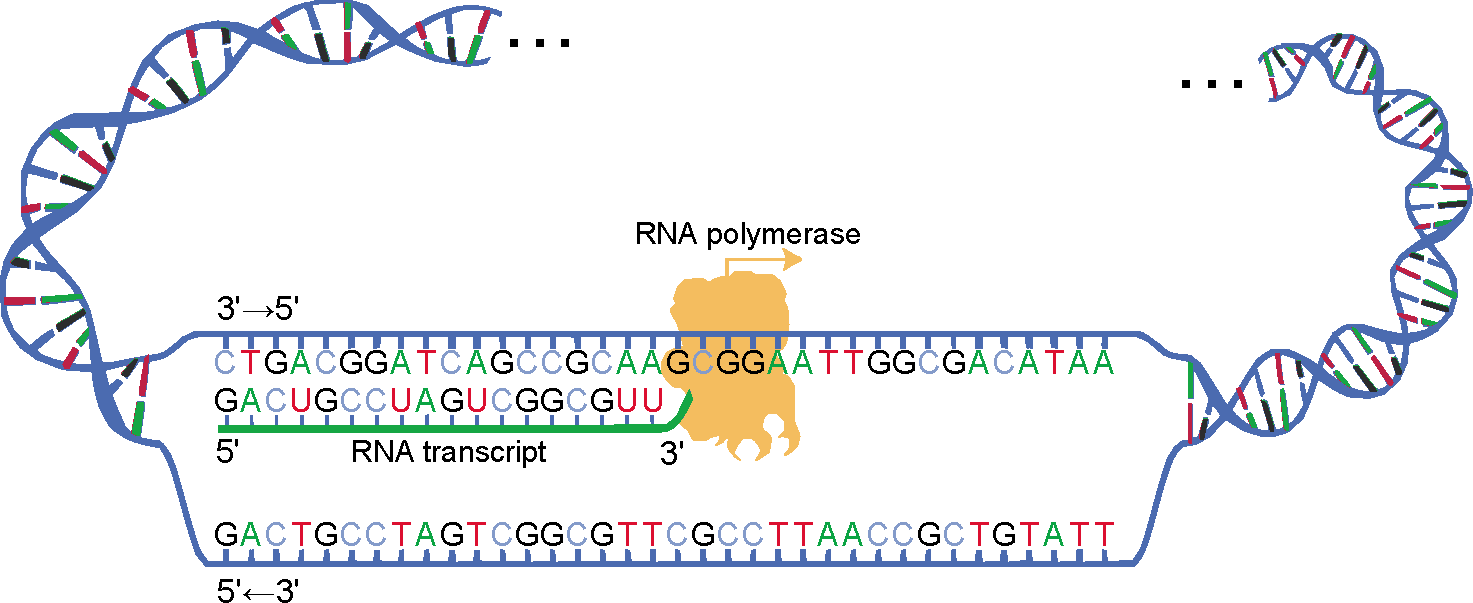
\includegraphics[width=1.00\textwidth]{imgs/dna_transcription.pdf}
	\caption[Transcription of DNA to RNA]{Transcription of DNA to RNA. The direction $3' \to 5'$ (or $5' \leftarrow 3'$, respectively) denotes the possible transcription direction on the \gls{DNA} strand. (adapted from \url{http://commons.wikimedia.org/wiki/File:DNA_transcription.svg}, public domain)}
	\label{fig:transcription}
\end{figure}

\gls{RNA} is produced with the help of \gls{DNA} using an enzyme (see glossary) called \emph{RNA polymerase}, illustrated in \cref{fig:transcription}. In this process, called \emph{transcription}, the \gls{RNA} is produced by forming the backbone bonds between newly created nucleotides. Their identity is determined by the sequence of nucleotides on the \gls{DNA}. Hence, the \gls{RNA} sequence is a faithful ``transcription'' of the \gls{DNA} sequence. More precisely, one of the two strands of the \gls{DNA} double strand is transcribed in direction $3' \to 5'$ such that the \gls{RNA} nucleotides are complements to the \gls{DNA} nucleotides: A $\to$ U, G $\to$ C, C $\to$ G, T $\to$ A. As seen in \cref{fig:transcription}, the transcription process produces reversed nucleotides, which means the $5'$ and $3'$ ends are opposite to those of the \gls{DNA} strand. After finishing the transcription process, the first level of organization can be described as the sequence of bases -- the primary structure. \Cref{fig:primary_struc} shows an example of such structure.

\begin{figure}
	\centering
	\begin{tikzpicture}[rna secondary structure]
		\begin{scope}[dot bracket]
			\node {C};
			\node {A};
			\node {A};
			\node {U};
			\node {U};
			\node {U};
			\node {U};
			\node {C};
			\node {U};
			\node {G};
			\node {A};
			\node {A};
			\node {A};
			\node {A};
			\node {U};
			\node {U};
			\node {U};
			\node {U};
			\node {C};
			\node {A};
			\node {C};
		\end{scope}
	\end{tikzpicture}
	\caption[Example of a primary structure]{Primary structure of a part of the tobacco etch virus (see \url{http://www.ekevanbatenburg.nl/PKBASE/PKB00279.HTML}).}
	\label{fig:primary_struc}
\end{figure}

\begin{figure}
	\centering
	\begin{tikzpicture}[rna secondary structure]
		\begin{scope}[natural]
			\node {C};
			\node[yshift=10pt,xshift=5pt] {A};
			\node[yshift=22pt,xshift=-5pt] {A};
			\node[yshift=23pt,xshift=-3pt] {U};
			\node[yshift=20pt,xshift=-1pt] {U};
			\node[yshift=16pt,xshift=0pt] {U};
			\node[yshift=10pt,xshift=5pt] {U};
			\node[yshift=-5pt,xshift=5pt] {C};
			\node[yshift=-15pt,xshift=0pt] {U};
			\node[continue chain=going below] {G};
			\node[yshift=-10pt,continue chain=going left] {A};
			\node[xshift=-5pt,join=with chain-6 by {basepair edge}] {A};
			\node[yshift=-10pt,join=with chain-5 by {basepair edge}] {A};
			\node[yshift=-20pt,xshift=5pt,join=with chain-4 by {basepair edge}] {A};
			\node[continue chain=going below,join=with chain-3 by {basepair edge}] {U};
			\node[yshift=-15pt,continue chain=going right,join=with chain-2 by {basepair edge}] {U};
			\node[xshift=5pt] {U};
			\node[yshift=10pt,xshift=5pt,join=with chain-11 by {basepair edge}] {U};
			\node[yshift=10pt,xshift=5pt,join=with chain-10 by {basepair edge}] {C};
			\node[yshift=6pt,xshift=5pt,join=with chain-9 by {basepair edge}] {A};
			\node[yshift=-6pt,xshift=5pt] {C};
		\end{scope}
	\end{tikzpicture}
	\caption[Example of a spring-model-style graph representing a secondary structure]{Spring-model-style graph representing the secondary structure belonging to \cref{fig:primary_struc}. Thin edges mark the backbone, while thick edges represent base pairs.}
	\label{fig:classical_sec_struc}
\end{figure}


\begin{figure}
	\centering
	\begin{tikzpicture}[rna secondary structure]
		\begin{scope}[linear]
			\node {C};
			\node {A};
			\node {A};
			\node {U};
			\node {U};
			\node {U};
			\node {U};
			\node {C};
			\node {U};
			\node {G};
			\node {A};
			\node[join=with chain-6 by {basepair edge}] {A};
			\node[join=with chain-5 by {basepair edge}] {A};
			\node[join=with chain-4 by {basepair edge}] {A};
			\node[join=with chain-3 by {basepair edge}] {U};
			\node[join=with chain-2 by {basepair edge}] {U};
			\node {U};
			\node[join=with chain-11 by {basepair edge}] {U};
			\node[join=with chain-10 by {basepair edge}] {C};
			\node[join=with chain-9 by {basepair edge}] {A};
			\node {C};
		\end{scope}
	\end{tikzpicture}
	\caption[Example of a linearized graph representing a secondary structure]{(Backbone-)Linearized graph representing the secondary structure belonging to \cref{fig:primary_struc}. As in \cref{fig:classical_sec_struc}, thin edges mark the backbone, while thick edges represent base pairs.}
	\label{fig:linear_sec_struc}
\end{figure}

\begin{figure}
	\centering
	\begin{tikzpicture}[rna secondary structure]
		\begin{scope}[dot bracket primary]
			\node {C};
			\node {A};
			\node {A};
			\node {U};
			\node {U};
			\node {U};
			\node {U};
			\node {C};
			\node {U};
			\node {G};
			\node {A};
			\node {A};
			\node {A};
			\node {A};
			\node {U};
			\node {U};
			\node {U};
			\node {U};
			\node {C};
			\node {A};
			\node {C};
		\end{scope}
		\begin{scope}[dot bracket,yshift=-0.5cm]
			\node {.};
			\node {(};
			\node {(};
			\node {(};
			\node {(};
			\node {(};
			\node {.};
			\node {.};
			\node {[};
			\node {[};
			\node {[};
			\node {)};
			\node {)};
			\node {)};
			\node {)};
			\node {)};
			\node {.};
			\node {]};
			\node {]};
			\node {]};
			\node {.};
		\end{scope}
	\end{tikzpicture}
	\caption[Example of the dot-bracket notation for a secondary structure]{Dot-bracket notation derived from \cref{fig:linear_sec_struc}. Dots are unpaired bases, while matching brackets are base pairs.}
	\label{fig:dot_bracket_sec_struc}
\end{figure}

In the salty cytoplasm of a cell -- or in vitro in salty water -- certain bases of the \gls{RNA} chain move together to form hydrogen bonds between each other. A bond is called a \emph{base pair} and can occur between A and U, G and C, or G and U. The second level of organization is therefore the set of base pairs that have formed -- the secondary structure. \Cref{fig:classical_sec_struc,fig:linear_sec_struc,fig:dot_bracket_sec_struc} show common ways for visualizing secondary structures. One distinctive property of a secondary structure is whether it is \emph{pseudoknotted}. A secondary structure is pseudoknotted if there are base pair edges that cross each other when displayed as a linearized graph. \Cref{fig:linear_sec_struc} shows such structure. The majority of RNA molecules are not pseudoknotted, yet a growing number of pseudoknotted structures have been found which are crucial for biological function \citep[cf.][]{reidys_topology_2011}.

Once the secondary structure has formed and some other conditions like a certain temperature \citep[cf.][]{ignacio_how_1999} are satisfied, the \gls{RNA} molecule transitions to a three-dimensional structure\footnote{In cells, the formation of a three-dimensional structure happens together with forming the secondary structure, as the conditions for both processes are always satisfied.}. Therefore, the third level of organization is the set of all atomic positions -- the tertiary structure.

It should be noted that the secondary and tertiary structures are formed according to chemical thermodynamics, meaning that each possible structure has a certain \emph{free energy} and that the structure formation process converges to those structures that have the \emph{lowest} free energy -- being the energetically \emph{most stable} structures \citep{ignacio_how_1999}.

This section is concluded by shortly describing two related areas of research where secondary structure prediction plays an important role.

As already mentioned, the function of an \gls{RNA} molecule depends on its tertiary structure. A common task is finding recurrent motifs in it -- as identical motifs could lead to identical functions. There are various physical methods to determine the tertiary structure, for example, X-ray crystallography or nuclear magnetic resonance spectroscopy. As the usage of such methods can be expensive and time-consuming, theoretical models have been developed that approximate tertiary structures, often with the help of secondary structures -- called \emph{hierarchical folding}. These models resulted in tools that have been used to describe certain motifs long before they had been validated by physical methods. See \citet[sect. 5.3]{meyers_rna_2000} for some examples.

A relatively new field of research lies in \emph{designing} \gls{RNA} molecules which have certain functions (e.g. cleaving \gls{RNA} virus particles to prevent infections). The problem here is finding an RNA primary structure that folds into a given tertiary (or as approximation secondary) structure. This problem is called \emph{inverse RNA folding} and is solved by enumerating all base pair matching primary structures and choosing the one which folds into a tertiary (secondary) structure with least free energy. For the latter part, existing tertiary (secondary) structure prediction algorithms can be employed. See \citet{andronescu_new_2004} for an introduction.

\section{Formalization as an Optimization Problem}
\label{sec:rna_optimization_problem}

Predicting secondary structures can be formalized as a combinatorial optimization problem. Solving it is enumerating all secondary structures from a search space, rating each structure using a certain free energy model, and returning those which have the lowest free energy.
Although eventually a single problem, secondary structure prediction is a family of optimization problems -- as many models exist that define the search space and scoring functions in certain ways with the goal of achieving better approximations or limiting computational complexity. The following overview provides a textual description of this family.

\begin{description}
	\item[Search space] All secondary structures which satisfy certain constraints:
		\begin{itemize}
			\item Match the given primary structure
			\item Allow only G-C, A-U, G-U base pairs
		\end{itemize}
\end{description}

Additional constraints further restricting the search space size are often used to lower the computational effort -- while trying to still consider most of the structures occurring in nature \citep{reidys_topology_2011}. Pseudoknotted structures play an important role here. As many \gls{RNA} molecules are in fact not pseudoknotted, the search space is often restricted to pseudoknot-free structures. Considering all pseudoknotted structures and using nontrivial\footnote{A trivial scoring function is the number of base pairs -- equivalent to the \emph{maximum weighted matching} graph problem which is solvable in polynomial time. Nontrivial scoring functions take the context of base pairs into account, e.g. stacks of base pairs are scored higher.} scoring functions leads to optimization problems that are NP-complete \citep{lyngso_rna_2000}. In this work, pseudoknot-free but also a restricted class of pseudoknotted structures, here named $C2u$ structures, are considered. It should be mentioned that, by convention, classes of some pseudoknotted structures always include all pseudoknot-free structures. The restricted class of pseudoknotted structures that is used in this work is defined in the following. Beginning with the class of unrestricted structures, a series of subsequent restrictions eventually leads to the class of $C2u$ structures.

Let $A = a_1 a_2 \ldots a_n$ be an RNA primary structure. Then, all base pairs that can theoretically form according to the base pairing rules are expressed as a set of pairs of indices:
\begin{equation}
	P = \{ (i,j) \mid 1 \leq i < j \leq n \wedge \text{$(a_i,a_j)$ is a base pair} \}.
\end{equation}

Given a set $s \in \mathbb{P}(P)$ of pairs of indices, then $\op{degree}(s,i)$ denotes how often the index $i$ is occurring in $s$.

The class of unrestricted structures contains all pseudoknotted and pseudoknot-free structures and is defined as the set of all combinations of base pairs such that each base takes part in at most one base pairing:
\begin{equation}
\label{eq:class_u}
	S_U = \{ s \in \mathbb{P}(P) \mid \forall (i,j) \in s. \op{degree}(s,i)=\op{degree}(s,j)=1 \}.
\end{equation}

In order to simplify further definitions, the concept of a \emph{shadow} is borrowed from \citet{reidys_topology_2011}. The shadow of any secondary structure displayed as linearized graph is obtained by removing all unpaired bases and noncrossing base pairs, and collapsing all uninterrupted stacks of base pairs into a single base pair. In the following, the function $\op{shadow} : \mathbb{P}(\mathbb{N}^2) \to \mathbb{P}(\mathbb{N}^2)$ is used as the operation transforming a secondary structure into its shadow. See \cref{fig:shadow} for an example. Using shadows, the class of pseudoknot-free structures can be defined as
\begin{equation}
	S_{PKF} = \{ s \in S_U \mid \op{shadow}(s) = \emptyset \}.
\end{equation}

\begin{figure}
	\centering
	\begin{tikzpicture}[rna secondary structure,transform shape,scale=0.55]
		\begin{scope}[linear]
			\node {};
			\node {};
			\node {};
			\node {};
			\node[join=with chain-3 by {basepair edge}] {};
			\node[join=with chain-4 by {basepair edge}] {};
			\node {};
			\node {};
			\node {};
			\node {};
			\node {};
			\node {};
			\node {};
			\node {};
			\node[join=with chain-7 by {basepair edge}] {};
			\node[join=with chain-2 by {basepair edge}] {};
			\node[join=with chain-1 by {basepair edge}] {};
			\node {};
			\node {};
			\node[join=with chain-19 by {basepair edge}] {};
			\node[join=with chain-18 by {basepair edge}] {};
			\node {};
			\node {};
			\node[join=with chain-13 by {basepair edge}] {};
			\node[join=with chain-12 by {basepair edge}] {};
			\node[join=with chain-11 by {basepair edge}] {};
		\end{scope}
		
		\begin{scope}[linear,xshift=20cm]
			\node {};
			\node {};
			\node {};
			\node[join=with chain-2 by {basepair edge}] {};
			\node[join=with chain-3 by {basepair edge}] {};
			\node {};
			\node {};
			\node[join=with chain-6 by {basepair edge}] {};
			\node[join=with chain-1 by {basepair edge}] {};
			\node[join=with chain-7 by {basepair edge}] {};
		\end{scope}
	\end{tikzpicture}
	\caption[Example of a secondary structure and its shadow]{Example of a secondary structure (left) and its shadow (right).}
	\label{fig:shadow}
\end{figure}

Before introducing the next class of secondary structures, the notion of \emph{connected components} is introduced \citep{reidys_topology_2011}. A set $C$ of base pairs is called a connected component if for any two base pairs $c,c' \in C$ there is a sequence of base pairs $c c_1 \ldots c_n c'$ with $c_1,\ldots,c_n \in C$ and $n \geq 0$ such that consecutive base pairs cross each other when displayed as linearized graph. Every base pair in a secondary structure or a shadow belongs to exactly one such component. Applied to the secondary structure in \cref{fig:shadow}, there are four such components (remember that each uncrossed base pair counts as a component), while its shadow only contains two components. Given a secondary structure or shadow, the function $\op{connectedComponents} : \mathbb{P}(\mathbb{N}^2) \to \mathbb{P}(\mathbb{P}(\mathbb{N}^2))$ returns those components. 

The next class of secondary structures -- here named $C2$ -- is now introduced. $C2$ structures are those where the shadows of all connected components are only allowed to be the most simplest ones -- those having at most two base pairs:
\begin{equation}
	S_{C2} = \{ s \in S_U \mid \forall c \in \op{connectedComponents}(s).|\op{shadow}(c)| \leq 2 \}.
\end{equation}

The secondary structure in \cref{fig:shadow} is an example of a $C2$ structure. The connected components of $C2$ structures are either single uncrossed base pairs or two groups of base pairs crossing each other. The functions $\op{leftGroup}$ and $\op{rightGroup}$ with signature $\mathbb{P}(\mathbb{N}^2) \to \mathbb{P}(\mathbb{N}^2)$ access the base pairs of those two groups of the latter type of components:
\begin{align}
	\op{leftGroup}(s) = \{ (i,j) \in s \mid \exists (k,l) \in s. i<k<j<l \}\\
	\op{rightGroup}(s) = \{ (k,l) \in s \mid \exists (i,j) \in s. i<k<j<l \}
\end{align}

Finally, the class $C2u$ is defined whose structures only contain connected components that are either single uncrossed base pairs or two groups of uninterrupted stacks of base pairs:
\begin{equation}
	S_{C2u} = \left\{ s \in S_{C2} \;\middle\vert\;
	\begin{aligned}
		&\forall c \in \op{connectedComponents}(s).\\
		& |c| \geq 2 \to\\
		&\forall g \in \{ \op{leftGroup}(c),\op{rightGroup}(c) \}.\\
		 & \max_{(i,j) \in g} i - \min_{(i,j) \in g} i
		 = |g|-1 =
		 \max_{(i,j) \in g} j - \min_{(i,j) \in g} j
	\end{aligned}
  \right\}
\end{equation}

\begin{figure}
	\centering
	\begin{tikzpicture}[rna secondary structure,transform shape,scale=0.55]
		\begin{scope}[linear]
			\node {};
			\node {};
			\node {};
			\node {};
			\node {};
			\node {};
			\node {};
			\node {};
			\node[join=with chain-6 by {basepair edge}] {};
			\node[join=with chain-7 by {basepair edge}] {};
			\node {};
			\node {};
			\node {};
			\node {};
			\node {};
			\node {};
			\node[join=with chain-14 by {basepair edge}] {};
			\node[join=with chain-16 by {basepair edge}] {};
			\node[join=with chain-15 by {basepair edge}] {};
			\node[join=with chain-4 by {basepair edge}] {};
			\node[join=with chain-3 by {basepair edge}] {};
			\node[join=with chain-2 by {basepair edge}] {};
			\node[join=with chain-1 by {basepair edge}] {};
			\node {};
			\node {};
			\node {};
			\node {};
			\node[join=with chain-25 by {basepair edge}] {};
			\node {};
			\node[join=with chain-24 by {basepair edge}] {};			
			\node[join=with chain-13 by {basepair edge}] {};
			\node[join=with chain-12 by {basepair edge}] {};
			\node[join=with chain-11 by {basepair edge}] {};
		\end{scope}
	\end{tikzpicture}
	\caption[Example of a $C2u$ secondary structure]{Example of a $C2u$ secondary structure.}
	\label{fig:c2u}
\end{figure}

\Cref{fig:c2u} as well as the earlier \cref{fig:linear_sec_struc} represent members of this class. The class of $C2u$ structures is a superset of the class of \emph{canonized simple recursive pseudoknot} structures from \citet{reeder_design_2004}\footnote{In fact, $C2u$ structures equal \emph{simple recursive pseudoknot} structures with only the first canonization rule from \citet{reeder_design_2004} applied.}.

\begin{description}
	\item[Scoring function] Each candidate of the search space is scored, e.g. by:
		\begin{itemize}
			\item Thermodynamic models \citep{zuker_optimal_1981,mathews_expanded_1999}
			\item Number of base pairs \citep{nussinov_algorithms_1978}
		\end{itemize}
\end{description}

The scoring function is the heart of the optimization problem and determines the accuracy of the solution. Free energy is modelled as a sum of contributions for small features in a structure. Giving weight to base pairs was the first and simplest model developed \citep{nussinov_algorithms_1978}, using the approximation that free energy gets lower when the number of base pairs gets higher. Newer more realistic models, called thermodynamic models, take certain motifs into account and actually calculate an approximation of the real free energy. Throughout this work, the number of base pairs is used as scoring function. Although not used any more for biological research, this method is easily understandable and known by anyone developing secondary structure prediction algorithms.

\pagebreak

\begin{description}
	\item[Solution] Finding those candidates whose score is minimal/maximal, e.g.:
		\begin{itemize}
			\item Minimization if scoring function returns free energy 
			\item Maximization if scoring function returns number of base pairs
		\end{itemize}
\end{description}

The solution of a secondary structure prediction problem is not always as simple as above. Due to the approximations used, biologists need to analyse suboptimal candidates too. Having a rated and ordered list of candidates, the solution might consist of the first ten candidates. In this work, only the simple types of solutions are considered -- as the extension to complex ones is not specific to the new approach of this thesis and directly carries over from existing work by \citet{sauthoff_bellmans_2011-1}.

\chapter{\texorpdfstring{Algebraic Dynamic Programming for Context-Free Languages}{ADP-CFL}}
\label{ch:adp-cfl}

\Gls{ADP} was introduced by \citet{giegerich_discipline_2004} and described as a discipline of dynamic programming over sequence data. It uses grammars and algebras as higher level abstractions to circumvent writing dynamic programming equations and corresponding algorithms while providing transformation rules to automatically derive both artefacts again. Working only on sequences, it can also be described as a way of (context-free) parsing over algebras (cf. semiring parsing by \citet{goodman_semiring_1999}).

\Gls{ADP} has been used primarily in the world of \gls{bioinformatics} to simplify writing software like \gls{RNA} secondary structure prediction tools \citep{reeder_design_2004,giegerich_abstract_2004,theis_prediction_2010}. Several software libraries exist that implement \gls{ADP} and thus provide a way to write grammars and algebras in source code. Depending on the implementation, the grammars can either be directly executed (interpreters) or are translated into dynamic programming equations which are further translated into a target language like C (compilers). At the time of writing, there exist five known implementations of \gls{ADP}: two interpreters (\emph{Haskell-ADP} by \citet{giegerich_discipline_2004}, and \emph{ADPfusion} by \citet{honer_zu_siederdissen_sneaking_2012}), two compilers (\emph{ADPC} by \citet{steffen_compiling_2006}, and \emph{GAPC} by \citet{sauthoff_bellmans_2011}), and a run-time code generator and compiler (\emph{DynaProg} by \citet{coppey_dynaprog_2012}).

This chapter introduces the concepts of \gls{ADP} and serves as the base for the following chapter where \gls{ADP} is redefined. To distinguish between the original definition of \gls{ADP} and its redefinition, the former is further named \gls{ADP-CFL}, and the latter \gls{ADP-MCFL}, designating the class of formal languages that each formalism is able to handle.

\section{Context-Free Grammars}
\label{sec:cfgs}

ADP-CFL has a direct correspondence to \glspl{CFG}. As \cref{sec:yield_parsing} details, the class of \emph{yield languages} that ADP-CFL recognizes is equivalent to the class of languages generated by \glspl{CFG}. In addition, it is trivial to transform a \gls{CFG} to the grammar form used in ADP-CFL (regular tree grammars) and vice versa -- the only difference being that \glspl{CFG} only generate derivation trees while ADP-CFL, imprecisely said, also evaluates each tree and aggregates their values. In order to have a common understanding of \glspl{CFG}, a short introduction follows.

\begin{definition}[Alphabet, words]
  \label{def:alphabetwords}
	An \emph{alphabet} $\mathcal{A}$ is a finite set of symbols. Sequences of symbols are called \emph{words}. The symbol $\epsilon$, which must not be part of an alphabet, denotes the empty word.
	The set of words with length $n$ over an alphabet $\mathcal{A}$ is defined by $\mathcal{A}^0 = \{\epsilon\}$, $\mathcal{A}^1 = \mathcal{A}$, and $\mathcal{A}^{n+1} = \{ ax \mid a \in \mathcal{A}, x \in \mathcal{A}^n \}$. The set of words with arbitrary lengths is $\mathcal{A}^* = \bigcup_{n \geq 0} \mathcal{A}^n$.
\end{definition}

A \gls{CFG} -- developed by \citet{chomsky_certain_1959} -- can be described \citep[sect. 6.1]{kastens_modellierung:_2008} as a tuple $\mathcal{G} = (V, \mathcal{A}, Z, P)$ where $V$ is an alphabet of nonterminal symbols, $\mathcal{A}$ an alphabet of terminal symbols disjoint from $V$, $Z \in V$ the start symbol, and $P$ a finite set of productions of the form $v \to r$ with $v \in V$ and $r \in (\mathcal{A} \cup V)^*$. By convention, multiple productions $v \to r_1, \ldots, v \to r_n$  with the same left-hand side can be written in compact form as $v \to r_1 \mid \ldots \mid r_n$.

Given a \gls{CFG} $\mathcal{G} = (V, \mathcal{A}, Z, P)$, then a nonterminal $v \in V$ in an arbitrary word $m = a v c \in (V \cup \mathcal{A})^*$ can be replaced by the right-hand side of a production $v \to b$ leading to $n = a b c \in (V \cup \mathcal{A})^*$. This is called a \emph{derivation step} and is written as $m \Rightarrow_\mathcal{G} n$. For any $m,n \in (V \cup \mathcal{A})^*$, $m \Rightarrow^*_\mathcal{G} n$ is called a \emph{derivation} if $m=n$ or if derivation steps $m \Rightarrow_\mathcal{G} d_1 \Rightarrow_\mathcal{G} \ldots \Rightarrow_\mathcal{G} d_k \Rightarrow_\mathcal{G} n$ exist for $k \geq 0$. Thus, the derivation relation $\Rightarrow^*_\mathcal{G}$ is the reflexive transitive closure of $\Rightarrow_\mathcal{G}$. When clear from the context, the subscript $\mathcal{G}$ can be omitted from $\Rightarrow_\mathcal{G}$ and $\Rightarrow^*_\mathcal{G}$.

\begin{definition}[Formal language]
  \label{def:formallanguage}
	A \emph{formal language}, or short \emph{language} in the context of words, is a set of words.
\end{definition}

\glsreset{CFL}

The language of a \gls{CFG} $\mathcal{G} = (V, \mathcal{A}, Z, P)$ is the set $\mathcal{L}(\mathcal{G}) = \{ w \in \mathcal{A}^* \mid Z \Rightarrow^* w \}$. A language $\mathcal{L}$ is said to be a \gls{CFL} if a \gls{CFG} $\mathcal{G}$ exists such that $\mathcal{L} = \mathcal{L}(\mathcal{G})$.

\begin{definition}[Tree]
  \label{def:tree}
  A \emph{tree} is a cycle-free \emph{directed graph} (see glossary) with a designated \emph{root} node, such that (a) only the root has in-degree 0, (b) every node is accessible from the root, and (c) all nodes except the root have in-degree 1.
  Nodes with out-degree 0 are called \emph{leaves}, all others \emph{inner nodes}.
  A tree is \emph{ordered} if the set of children of each node is assigned a total order.
  A tree is \emph{labelled} if each node is assigned a label.
\end{definition}

\begin{definition}[Derivation tree of \glspl{CFG}]
  \label{def:derivtree_cfg}
	An ordered tree $T$ with labels $m : T \to \mathcal{A} \cup \{\epsilon\} \cup V$ is a derivation tree for a \gls{CFG} $\mathcal{G}=(V, \mathcal{A}, Z, P)$, if
	\begin{itemize}[noitemsep]
		\item every inner node $k$ of $T$ satisfies $m(k) \in V$,
		\item every leaf $l$ of $T$ satisfies $m(l) \in \mathcal{A} \cup \{\epsilon\}$,
		\item the root $r$ of $T$ satisfies $m(r)=Z$,
		\item every inner node $k$ of $T$ with children $k_1,\ldots,k_n$ satisfies\\ $m(k) \to m(k_1) \ldots m(k_n) \in P$, and
		\item every inner node $k$ of $T$ with a single child $k_1$ with $m(k_1)=\epsilon$ satisfies $m(k) \to \epsilon \in P$.\qedhere
	\end{itemize}	
\end{definition}

A derivation tree can represent multiple derivations, depending on the order in which the derivation steps are applied. Therefore, a derivation tree abstracts from the order in which it was constructed. A \gls{CFG} is called \emph{ambiguous} if multiple derivation trees exist that yield the same word.

\begin{definition}[Formal tree language]
  \label{def:formaltreelanguage}
	A \emph{formal tree language}, or short \emph{language} in the context of trees, is a set of trees.
\end{definition}

The language $\mathcal{L}_T(\mathcal{G})$ of a \gls{CFG} $\mathcal{G}= (V, \mathcal{A}, Z, P)$ is the set of all derivation trees that can be created from derivations $Z \Rightarrow^* w$ with any $w \in \mathcal{A}^*$. The set of derivation trees that can be created from derivations $Z \Rightarrow^* w$ with a given $w \in \mathcal{A}^*$ is denoted $\mathcal{Q}_\mathcal{G}(w)$.


\begin{example}[\gls{CFG} for pseudoknot-free \gls{RNA} secondary structures]
	\label{ex:cfg_pkf}
	When building grammars for \gls{RNA} secondary structures, one has to take the exact opposite approach as in \autoref{sec:rna_optimization_problem}. In that section, the sets of structures were constructed by gradually restricting the search space. Here, the search space -- which equals the set of possible derivation trees -- has to be built from the ground up by defining exactly those productions that \emph{generate} the desired derivation trees.
	
	It is often easier when creating grammars for \gls{RNA} secondary structures to think in terms of words of the dot-bracket notation. Then, the search space is the set of derivable words instead of the set of derivation trees. The dot-bracket grammar that recognizes all pseudoknot-free secondary structures is readily given by $\mathcal{G}_{PKF-DB}=(\{Z\},\{\ts{(},\ts{)},\ts{.}\},Z,P_{PKF-DB})$ with 
	\[ P_{PKF-DB}=\{Z \to \ts{.}Z \mid \ts{(}Z\ts{)}Z \mid \epsilon\}. \]
	
	For each word produced by $\mathcal{L}(\mathcal{G}_{PKF-DB})$, exactly one derivation tree exists. The derivation trees for \ts{.....} and \ts{(.())} are shown in the following:
	
	\begin{spreadTrees}
		% ..... -> Z(.,Z(.,Z(.,Z(.,Z(.,Z(\epsilon))))))
		\Tree [.$Z$ \ts{.} [.$Z$ \ts{.} [.$Z$ \ts{.} [.$Z$ \ts{.} [.$Z$ \ts{.} [.$Z$ $\epsilon$ ] ] ] ] ] ]
		%	(.()) -> Z('(',Z(.,Z('(',Z(\epsilon),')',Z(\epsilon))),')',Z(\epsilon))
		\Tree [.$Z$ \ts{(} [.$Z$ \ts{.} [.$Z$ \ts{(} [.$Z$ $\epsilon$ ] \ts{)} [.$Z$ $\epsilon$ ] ] ] \ts{)} [.$Z$ $\epsilon$ ] ]
	\end{spreadTrees}
	
	To give an example of a derivation, one possible derivation corresponding to the right derivation tree is given:
	\begin{equation*}
	 Z \Rightarrow
	 \ts{(} Z \ts{)} Z \Rightarrow
	 \ts{(} \ts{.} Z \ts{)} Z \Rightarrow
	 \ts{(} \ts{.} \ts{(} Z \ts{)} Z \ts{)} Z \Rightarrow
	 \ts{(} \ts{.} \ts{(} \ts{)} Z \ts{)} Z \Rightarrow
	 \ts{(} \ts{.} \ts{(} \ts{)} \ts{)} Z \Rightarrow
	 \ts{(.())}
	\end{equation*}

	This (unambiguous) grammar just recognizes secondary structures instead of generating all such structures from a given primary structure. The transformation to a suitable (ambiguous) grammar although is easy: productions with a dot have to be expanded to multiple productions where the dot is replaced by all the bases, and productions with a pair of brackets have to be expanded to productions with base pairs. In grammar	$\mathcal{G}_{PKF'} = (\{Z\}, \mathcal{A}_{RNA},Z,P_{PKF'})$ with $\mathcal{A}_{RNA} = \{\ts{a},\ts{g},\ts{c},\ts{u}\}$ this transformation was applied:	
	\begin{align*}
		P_{PKF'} = &\{&&\\
		&&Z &\to \ts{a}Z \mid \ts{u}Z \mid \ts{g}Z \mid \ts{c}Z \mid \ts{a}Z\ts{u}Z \mid \ts{u}Z\ts{a}Z \mid\\
		&&&\mathrel{\phantom{\to}} \ts{g}Z\ts{c}Z \mid \ts{c}Z\ts{g}Z \mid \ts{g}Z\ts{u}Z \mid \ts{u}Z\ts{g}Z \mid \epsilon\\
		&\}.&&
	\end{align*}
	
	Now, for each word, multiple derivation trees exist. As an example, the following two trees are derived from the word \ts{agcgu}. Eight other derivation trees for \ts{agcgu} exist.
	
	\begin{spreadTrees}
		% ..... -> Z(a,Z(g,Z(c,Z(g,Z(u,Z(\epsilon))))))
		\Tree [.$Z$ \ts{a} [.$Z$ \ts{g} [.$Z$ \ts{c} [.$Z$ \ts{g} [.$Z$ \ts{u} [.$Z$ $\epsilon$ ] ] ] ] ] ]
		%	(.()) -> Z(a,Z(g,Z(c,Z(\epsilon),g,Z(\epsilon))),u,Z(\epsilon))
		\Tree [.$Z$ \ts{a} [.$Z$ \ts{g} [.$Z$ \ts{c} [.$Z$ $\epsilon$ ] \ts{g} [.$Z$ $\epsilon$ ] ] ] \ts{u} [.$Z$ $\epsilon$ ] ]
	\end{spreadTrees}
	
	Again, to give an example of a derivation, one possible derivation corresponding to the right derivation tree is given:
	\begin{equation*}
	 Z \Rightarrow
	 \ts{a} Z \ts{u} Z \Rightarrow
	 \ts{a} \ts{g} Z \ts{u} Z \Rightarrow
	 \ts{a} \ts{g} \ts{c} Z \ts{g} Z \ts{u} Z \Rightarrow
	 \ts{a} \ts{g} \ts{c} \ts{g} Z \ts{u} Z \Rightarrow
	 \ts{a} \ts{g} \ts{c} \ts{g} \ts{u} Z \Rightarrow
	 \ts{agcgu}
	\end{equation*}
	
	Introducing new nonterminals for base pairs and bases, the final grammar which is further used is given by $\mathcal{G}_{PKF} = (\{Z,P,B\}, \mathcal{A}_{RNA},Z,P_{PKF})$ with	
	\begin{align*}
		P_{PKF} = &\{&&\\
		&&Z &\to BZ \mid PZ \mid \epsilon,\\
		&&P &\to \ts{a}Z\ts{u} \mid \ts{u}Z\ts{a} \mid \ts{g}Z\ts{c} \mid \ts{c}Z\ts{g} \mid \ts{g}Z\ts{u} \mid \ts{u}Z\ts{g},\\
		&&B &\to \ts{a} \mid \ts{u} \mid \ts{g} \mid \ts{c}\\
		&\}.&&
	\end{align*}
	
	Of course, this whole transformation process would be pointless if the secondary structure that is somewhere hidden in the derivation tree -- and which was explicit in the dot-bracket notation -- could not be reconstructed. An easy way is to regard derivation trees as terms and assign each nonterminal a function that constructs a part of the secondary structure as dot-bracket notation word:	
	\begin{align*}
		Z(x,y) &= xy\\
		Z(\epsilon) &= \epsilon\\
		P(b_1,z,b_2) &= \ts{(}z\ts{)}\\
		B(x) &= \ts{.} \qedhere
	\end{align*}
\end{example}

\section{Regular Tree Grammars}
\label{sec:regular_tree_grammars}

The main component of ADP-CFL is a class of grammars called \emph{regular tree grammars} \citep{brainerd_tree_1969} -- a device to describe a set of ordered trees. Regular tree grammars are usually defined using ranked alphabets -- an alphabet, and a function assigning an arity to each symbol -- but for ADP-CFL it is useful to extend this concept to algebraic signatures. Using the latter, a fine-grained subclass of regular tree grammars can be defined by restricting grammars to only use certain algebraic signatures or classes thereof. In common definitions of ADP-CFL, this approach is used and specialized. In this section, regular tree grammars over algebraic signatures are introduced, while the following section defines the class of regular tree grammars used in ADP-CFL. From now on, the notions (ordered labelled) tree and term are used interchangeably.

In programming languages, types are used to guarantee the structural correctness of a term. For example, in Java, \verb|1 - true| is an invalid term as the minus operator is defined for numbers only. A similar concept is used in the field of universal algebra. A set of terms can be divided into disjoint sets where each set corresponds to a \emph{sort}. By restricting each argument of an operator to a sort, a basic (type) system for guaranteeing structural correctness is formed. Note that sorts are merely names -- in \cref{sec:adp_problem_solution}, when meaning is added to terms, sorts are assigned to domains.

\begin{definition}[Signature {\citep[cf.][Def. 3.1, 3.3]{kastens_modellierung:_2008}}]
  \label{def:signature}
	A (many-sorted) signature $\Sigma$ is a tuple $(S,F)$ where $S$ is a set of sorts, and $F$ a set of structural descriptions. A structural description describes an $n$-ary function or relation symbol $op$ and has the form $op: s_1 \times \ldots \times s_n \to s_0$ with $s_i \in S$.
\end{definition}

\begin{definition}[Algebraic signature]
  \label{def:alg_signature}
	A signature without relation symbols is called an \emph{algebraic signature}.
\end{definition}

\begin{definition}[Correct terms over a signature {\citep[Def. 3.4]{kastens_modellierung:_2008}}]
  \label{def:correct_terms}
	Given a signature $\Sigma =(S,F)$, then the set of \emph{correct terms} over $\Sigma$ contains the term $t$ of sort $s \in S$, if (a) $t$ is the name of a variable of sort $s$, or (b) $t = f (t_1,\ldots,t_n)$ with $n \geq 0$ where $F$ contains a structural description $f : s_1 \times \ldots \times s_n \to s_0$ such that every $t_i, 1 \leq i \leq n$ is a correct term of sort $s_i$.
\end{definition}

\begin{definition}[Ground term {\citep[Def. 3.5]{kastens_modellierung:_2008}}]
  \label{def:ground_term}
	A correct term without variables is called a \emph{ground term}.
\end{definition}

$T_\Sigma$ is the language containing all ground terms over $\Sigma$.
$T_\Sigma(V)$ is the language containing all correct terms over $\Sigma$ where all variables are from a set $V$.

\begin{definition}[Position of a variable]
	To each variable in a correct term a unique number called \emph{position} is assigned such that all variables in a term have distinct numbers.
\end{definition}

\pagebreak

\begin{definition}[Replacement of a variable]
	The replacement of a variable at position $p$ in term $t$ by $u$ is denoted $t[u]_p$.
\end{definition}

\begin{definition}[Regular tree grammar over an algebraic signature {\citep[cf.][sect. 3.4]{giegerich_code_1988}}] 
	\label{def:regular_tree_grammar}
	A regular tree grammar $\mathcal{G}$ over an algebraic signature $\Sigma$ is defined as a tuple $(V,\Sigma,Z,P)$, where $V$ is an alphabet of nonterminal symbols disjoint from function symbols in $\Sigma$, $Z \in V$ is the start symbol, and $P$ a finite set of productions which have the form $v \to t$ where $v \in V$ and $t \in T_\Sigma(V)$. All terms $t$ in productions $v \to t$ of the same nonterminal $v \in V$ must have the same sort.
\end{definition}

\begin{remark}
	In expression $T_\Sigma(V)$ of \cref{def:regular_tree_grammar}, the alphabet of nonterminals $V$ is regarded as a set of variables where the sort of each variable is determined by the right-hand sides of its corresponding productions.
\end{remark}

Given a regular tree grammar $\mathcal{G}=(V,\Sigma,Z,P)$, then a nonterminal $v \in V$ at position $p$ in a term $t \in T_\Sigma(V)$ can be replaced by the right-hand side of a production $v \to v' \in P$ leading to a new term $t'=t[v']_p$. This is called a \emph{derivation step} and is written as $t \Rightarrow_\mathcal{G} t'$. For any terms $m,n \in T_\Sigma(V)$, $m \Rightarrow^*_\mathcal{G} n$ is called a \emph{derivation} if $m=n$ or if derivation steps $m \Rightarrow_\mathcal{G} d_1 \Rightarrow_\mathcal{G} \ldots \Rightarrow_\mathcal{G} d_k \Rightarrow_\mathcal{G} n$ exist for $k \geq 0$. Thus, the derivation relation $\Rightarrow^*_\mathcal{G}$ is the reflexive transitive closure of $\Rightarrow_\mathcal{G}$. When clear from the context, the subscript $\mathcal{G}$ can be omitted from $\Rightarrow_\mathcal{G}$ and $\Rightarrow^*_\mathcal{G}$.

The language of a term $t \in T_\Sigma(V)$ is the set $\mathcal{L}(\mathcal{G},t) = \{ t' \in T_\Sigma \mid t \Rightarrow^* t' \}$. The language of $\mathcal{G}$ is the set $\mathcal{L}(\mathcal{G}) = \mathcal{L}(\mathcal{G},Z) = \{ t \in T_\Sigma \mid Z \Rightarrow^* t \}$. $\mathcal{L}(\mathcal{G})$ is a subset of $T_\Sigma$.

\begin{example}[Regular tree grammar for sequences of natural numbers]
	A regular tree grammar is given by $\mathcal{G}_{Nat} = (\{Seq,Nat\},\Sigma_{Nat},Seq,P_{Nat})$ where
	\begin{align*}
		P_{Nat} = &\{&&\\
			&&Seq &\to \op{nil} \mid \op{cons}(Nat,Seq), \\
			&&Nat &\to 0 \mid \op{s}(Nat)\\
		&\},&&
	\end{align*}
	and $\Sigma_{Nat}=(\{N,N^*\},F_{Nat})$ with
	\begin{align*}
		F_{Nat} = &\{&&&&\\
		&&\op{nil} &: \{()\} &&\to N^*,\\
		&&\op{cons} &: N \times N^* &&\to N^*,\\
		&&0 &: \{()\} &&\to N,\\
		&&\op{s} &: N &&\to N\\
		&\}.&&&&
	\end{align*}
		
	Some terms in $\mathcal{L}(\mathcal{G}_{Nat})$ are
	\begin{align*}
		&\op{nil},\\
		&\op{cons}(0,\op{nil}),\\
		&\op{cons}(\op{s}(\op{s}(\op{s}(0))),\op{cons}(\op{s}(0),\op{nil})).
	\end{align*}
	
	One possible derivation of the second term is given for illustration:
	\begin{equation*}
		Seq \Rightarrow 
		\op{cons}(Nat,Seq) \Rightarrow
		\op{cons}(0,Seq) \Rightarrow
		\op{cons}(0,\op{nil})
	\end{equation*}
	
	The relation to trees in tree grammars is made by imagining that instead of terms, trees are 
	generated:
	
	\begin{spreadTrees}
		\Tree [.nil ]
		\Tree [.cons 0 nil ]
		\Tree [.cons [.s [.s [.s 0 ] ] ] [.cons [.s 0 ] nil ] ]
	\end{spreadTrees}
\end{example}

An important lesson is that although trees implicitly exist as derivation trees for \glspl{CFG}, they were now made explicit in regular tree grammars. The concept of words though is lost now. In the next section, this concept is reintroduced to fuse the worlds of words and trees in a very explicit way.

\section{ADP-CFL Grammars}

As already mentioned, common definitions of ADP-CFL -- e.g. \citet{honer_zu_siederdissen_sneaking_2012,sauthoff_bellmans_2011,giegerich_discipline_2004} -- use a subclass of regular tree grammars . This is achieved by restricting the forms of algebraic signatures and productions that are allowed. The common usage of this subclass is not an inherent restriction of ADP-CFL but rather a way to reduce the complexity of further definitions. A remark in the end of this section elaborates on this further.

The simplified definition of ADP-CFL assumes that all nonterminals of a regular tree grammar generate terms of the same sort. It will later become clear that this restriction implies that only a single objective function can be used.

First, a subclass of algebraic signatures is introduced, in this work named \emph{grammar signatures}, following \citet[sect. 3.1]{giegerich_discipline_2004}. One of the purposes of this class is to introduce signatures with exactly two sorts where one sort is designated as the (terminal) \emph{alphabet sort}, and the other as the \emph{result sort}. Through this distinction, further definitions can reference both sorts explicitly.

\begin{definition}[Grammar signature]
	A grammar signature $\Sigma$ is a tuple $(\mathcal{A},\mathcal{S},F)$ which defines an algebraic signature $(\{\mathcal{A},\mathcal{S}\},F \cup F_\mathcal{A})$ where $\mathcal{S}$ is the result sort, and $\mathcal{A}$ is an alphabet of terminal symbols that is formally used as the alphabet sort but also for implicitly defining a set of structural descriptions $F_\mathcal{A}$ describing constant function symbols $a: \{()\} \to \mathcal{A}$ for each $a \in \mathcal{A}$. Additionally, each structural description $f \in F$ must have the form $f: s_1 \times \ldots \times s_n \to \mathcal{S}$ with $s_i \in \{\mathcal{A},\mathcal{S}\}$.\footnote{In \citet{giegerich_discipline_2004}, a non-standard definition of (single-sorted) signatures was used in which $\mathcal{A}$ is just a set of symbols rather than a proper sort. In this chapter, ADP-CFL is defined using regular definitions from the field of universal algebra.}
\end{definition}

\begin{definition}[Production term over a grammar signature]
	Given a grammar signature $\Sigma=(\mathcal{A},\mathcal{S},F)$, then a correct term over $\Sigma$ of sort $\mathcal{S}$ is called a \emph{production term}.
\end{definition}

Given a grammar signature $\Sigma$, then $T^p_\Sigma$ is the language containing all production terms over $\Sigma$ which are also ground terms.
$T^p_\Sigma(V)$ is the language containing all production terms over $\Sigma$ where all variables are from a set $V$.

Finally, a definition of the type of restricted regular tree grammars used in further definitions of ADP-CFL can be given.

\begin{definition}[ADP-CFL grammar over $\Sigma$ {\citep[cf.][Def. 1]{giegerich_discipline_2004}}]
	\label{def:tree_grammar}
	An ADP-CFL grammar $\mathcal{G}$ over a grammar signature $\Sigma=(\mathcal{A},\mathcal{S},F)$ is a tuple $(V,\mathcal{A},Z,P)$ and describes a regular tree grammar $(V,\Sigma,Z,P)$, where the productions in $P$ must have the form $v \to t$ with $v \in V$ and $t \in T^p_\Sigma (V)$.
\end{definition}

Observation: A regular tree grammar $\mathcal{G}$ over an algebraic signature $\Sigma$ with a single sort $S$ is an ADP-CFL grammar. This follows, when the result sort of the corresponding ADP-CFL grammar is mapped to $S$, and the alphabet set is empty so that the alphabet sort stays unused and can effectively be ignored. But it is the alphabet sort that is of utmost importance for the concept of ADP-CFL, which is why ADP-CFL is not simply defined as a regular tree grammar with a single sort. In the following section, the reason of this importance is explained.

\begin{remark}
	Although the restriction of each nonterminal generating terms of a single sort $\mathcal{S}$ seems to produce more formal work than necessary at the moment, it vastly reduces the complexity of definitions and methods in the rest of this work. The formal extension to multiple result sorts (and with that, multiple objective functions) is very briefly discussed in \citet[sect. 2.2.2]{sauthoff_bellmans_2011-1}. Also, note that all known implementations of ADP-CFL support multiple result sorts.	
	%with multiple result sorts we could do:
	%S -> f(B,S) \ldots h_1 =max        sort=S
	%B -> a | g | c | u [... h_2=id] sort=A
	%with a single result sort, we have to use a workaround:
	%B -> foo(a) | foo(g) | foo(c) | foo(u)  h1=max   sort=S
	%NOTE: adp-multi kann auch mehrere sorts
\end{remark}

Before providing an example of an ADP-CFL grammar for RNA secondary structures, the notion of yield parsing has to be introduced which relates terms of ADP-CFL grammars to words of a context-free language. With this relation, an ADP-CFL grammar which corresponds to the context-free grammar $\mathcal{G}_{PKF}$ of \cref{ex:cfg_pkf} can be constructed.
         
\section{Yield Parsing for ADP-CFL Grammars}
\label{sec:yield_parsing}

Given an ADP-CFL grammar $\mathcal{G}=(V,\mathcal{A},Z,P)$ over $\Sigma=(\mathcal{A},\mathcal{S},F)$, then its yield function $\op{y}_\mathcal{G} : T_\Sigma \to \mathcal{A}^*$ is defined as
\begin{equation}
	\label{eq:y}
	\op{y}_\mathcal{G}(z) = 
	\begin{cases}
		z & \text{if $z \in \mathcal{A}$,}\\
		\op{y}_\mathcal{G}(x_1)\ldots\op{y}_\mathcal{G}(x_n) & \text{if $z = f(x_1,\ldots,x_n), f \in F$.}
	\end{cases}
\end{equation}

By constructing ADP-CFL grammars whose generated trees have elements of $\mathcal{A}$ in their leaves, it is now possible to extract those elements and concatenate them to words.

\begin{example}[ADP-CFL grammar for sequences of characters]
	\label{ex:adp_cfl_chars}
	An ADP-CFL grammar is given by $\mathcal{G}_{Char} = (\{Seq,Char\},\mathcal{A},Seq,P)$ over $\Sigma$ where $\mathcal{A}=\{\ts{0},\ts{1},\ts{a},\ts{b}\}$,
	\begin{align*}
		P = &\{&&\\
			&&Seq &\to \op{nil} \mid \op{cons}(Char,Seq), \\
			&&Char &\to \op{number}(\ts{0}) \mid \op{number}(\ts{1}) \mid \op{letter}(\ts{a}) \mid \op{letter}(\ts{b})\\
		&\},&&
	\end{align*}
	and $\Sigma=(\mathcal{A},\mathcal{S},F)$ with
	\begin{align*}
		F = &\{&&&&\\
		&&\op{nil} &: \{()\} &&\to \mathcal{S},\\
		&&\op{cons} &: \mathcal{S} \times \mathcal{S} &&\to \mathcal{S},\\
		&&\op{number} &: \mathcal{A} &&\to \mathcal{S},\\
		&&\op{letter} &: \mathcal{A} &&\to \mathcal{S}\\
		&\}.&&&&
	\end{align*}
	
	Some terms in $\mathcal{L}(\mathcal{G}_{Char})$ with $\op{y}_{\mathcal{G}_{Char}}$ applied are:
	\begin{align*}
		&\op{y}_{\mathcal{G}_{Char}}(\quad\op{nil} \quad) &&= \epsilon\\
		&\op{y}_{\mathcal{G}_{Char}}(\quad\op{cons}(\op{number}(\ts{0}),\op{nil})\quad) &&= \ts{0}\\
		&\op{y}_{\mathcal{G}_{Char}}(\quad\op{cons}(\op{number}(\ts{0}),\op{cons}(\op{letter}(\ts{a}),\op{nil}))\quad) &&= \ts{0a} \qedhere
	\end{align*}
\end{example}

The yield language of a term $t \in T_\Sigma(V)$ is defined as 
\begin{equation}
	\mathcal{L}_{\op{y}}(\mathcal{G},t) = \{ \op{y}_\mathcal{G}(t') \mid t' \in \mathcal{L}(\mathcal{G},t) \}.
\end{equation}

The yield language of $\mathcal{G}$ is defined as 
\begin{equation}
	\mathcal{L}_{\op{y}}(\mathcal{G}) = \mathcal{L}_{\op{y}}(\mathcal{G},Z) = \{ \op{y}_\mathcal{G}(t) \mid t \in \mathcal{L}(\mathcal{G}) \}.
\end{equation}

The class of yield languages of ADP-CFL grammars is equivalent to the class of languages generated by context-free grammars \citep[Theorem 6]{giegerich_implementing_2002}.

\begin{example}[continues=ex:adp_cfl_chars]
	The yield language of the term $Char$ is equal to the set $\{\ts{0},\ts{1},\ts{a},\ts{b}\}$.
	The yield language of the term $Seq$ is equal to the set $\{\ts{0},\ts{1},\ts{a},\ts{b}\}^*$. The yield language of $\mathcal{G}_{Char}$ is the yield language of $Seq$.
\end{example}

Computing the inverse of the yield function is called yield parsing. The yield
parser $\mathcal{Q}_\mathcal{G}$ of an ADP-CFL grammar $\mathcal{G}$ computes the search space of all possible yield parses:
\begin{equation}
  \label{eq:yieldparsercfl}
	\mathcal{Q}_\mathcal{G}(x) = \{ t \in \mathcal{L}(\mathcal{G}) \mid \op{y}_\mathcal{G}(t) = x \}.
\end{equation}

\begin{example}[continues=ex:adp_cfl_chars]
	As in $\mathcal{G}_{Char}$ each term yields a unique word, the yield parser $\mathcal{Q}_{\mathcal{G}_{Char}}$ returns exactly the single term that is associated to the word.
	
	For the earlier examples
	\begin{align*}
		&\mathcal{Q}_{\mathcal{G}_{Char}}(\epsilon) &&= \{\op{nil}\},\\
		&\mathcal{Q}_{\mathcal{G}_{Char}}(\ts{0}) &&= \{\op{cons}(\op{number}(\ts{0}),\op{nil})\},\\
		&\mathcal{Q}_{\mathcal{G}_{Char}}(\ts{0a}) &&= \{\op{cons}(\op{number}(\ts{0}),\op{cons}(\op{letter}(\ts{a}),\op{nil}))\}.
	\end{align*}
\end{example}

The following example, which continues the running example of RNA secondary structure prediction, uses the concept of yield parsing for generating multiple terms for each word. The search space that was created by derivation trees of $\mathcal{G}_{PKF}$ is now replicated in the formalism of regular tree grammars -- or more specifically: ADP-CFL grammars. Only in the next section it will become clear what the actual benefit of this representation of the search space is.

\begin{example}[ADP-CFL grammar for pseudoknot-free \gls{RNA} secondary structures]
	\label{ex:treegrammar_pkf}
	In this example, the \gls{CFG} $\mathcal{G}_{PKF}$ from \cref{ex:cfg_pkf} is transformed to an ADP-CFL grammar $\mathcal{G}_{PKF-T}$ where, given a primary structure, the sets of derivable secondary structures from both grammars are equal. More formally, an ADP-CFL grammar needs to be found such that for every $x \in \mathcal{A}^*_{RNA}$ the sets of terms $\mathcal{Q}_{\mathcal{G}_{PKF-T}}(x)$ and $\mathcal{Q}_{\mathcal{G}_{PKF}}(x)$ are equivalent. In this context, two term sets are considered equivalent if both sets are equal when each term has been replaced by its dot-bracket notation word.
	
	Constructing such grammars with equivalent term set is straight-forward. Each production in $\mathcal{G}_{PKF}$ is transformed by using the symbols of the right-hand side as arguments of a new function symbol. As the argument types are either $\mathcal{A}$ or $\mathcal{S}$, the empty word is represented by an empty list of arguments, instead of a single argument with the empty word. Although each production could be constructed with a new function symbol, in this example a certain set of symbols are reused to group similar cases. In the following \cref{sec:adp_problem_solution} -- when terms are evaluated -- the rationale behind it will become clearer.
		
	The resulting ADP-CFL grammar is given by 
	\[ \mathcal{G}_{PKF-T} = (\{Z,P,B\},\mathcal{A},Z,P_{PKF-T}) \text{ over } \Sigma_{PKF-T} \] where $\mathcal{A} = \mathcal{A}_{RNA}$, 
	\begin{align*}
		P_{PKF-T} = &\{&&\\
		&&Z &\to \op{f}_1(B,Z) \mid \op{f}_2(P,Z) \mid \op{f}_3,\\
		&&P &\to \op{f}_4(\ts{a},Z,\ts{u}) \mid \op{f}_4(\ts{u},Z,\ts{a}) \mid \op{f}_4(\ts{g},Z,\ts{c}) \mid\\
		&&  &\mathrel{\phantom{\to}} \op{f}_4(\ts{c},Z,\ts{g}) \mid \op{f}_4(\ts{g},Z,\ts{u}) \mid \op{f}_4(\ts{u},Z,\ts{g}),\\
		&&B &\to \op{f}_5(\ts{a}) \mid \op{f}_5(\ts{u}) \mid \op{f}_5(\ts{g}) \mid \op{f}_5(\ts{c})\\
		&\},&&
	\end{align*}
	and $\Sigma_{PKF-T}=(\mathcal{A},\mathcal{S},F_{PKF-T})$ with \pagebreak
	\begin{align*}
		F_{PKF-T} = &\{&&&&\\
		&&\op{f}_1 &: \mathcal{S} \times \mathcal{S} &&\to \mathcal{S},\\
		&&\op{f}_2 &: \mathcal{S} \times \mathcal{S} &&\to \mathcal{S},\\
		&&\op{f}_3 &: \{()\} &&\to \mathcal{S},\\
		&&\op{f}_4 &: \mathcal{A} \times \mathcal{S} \times \mathcal{A} &&\to \mathcal{S},\\
		&&\op{f}_5 &: \mathcal{A} &&\to \mathcal{S}\\
		&\}.&&&&
	\end{align*}
	
	Two of ten trees of the set $\mathcal{Q}_{\mathcal{G}_{PKF-T}}(\ts{agcgu})$ are given:
  
	\begin{spreadTrees}
		% .....  -> f_1(f_5(a),f_1(f_5(g),f_1(f_5(c),f_1(f_5(g),f_1(f_5(u),f_3)))))
		\Tree [.$\op{f}_1$ [.$\op{f}_5$ \ts{a} ] [.$\op{f}_1$ [.$\op{f}_5$ \ts{g} ] [.$\op{f}_1$ [.$\op{f}_5$ \ts{c} ] [.$\op{f}_1$ [.$\op{f}_5$ \ts{g} ] [.$\op{f}_1$ [.$\op{f}_5$ \ts{u} ] $\op{f}_3$ ] ] ] ] ]	
		%	(.())	 -> f_2(f_4(a,f_1(f_5(g),f_2(f_4(c,f_3,g),f_3)),u),f_3)	
		\Tree [.$\op{f}_2$ [.$\op{f}_4$ \ts{a} [.$\op{f}_1$ [.$\op{f}_5$ \ts{g} ] [.$\op{f}_2$ [.$\op{f}_4$ \ts{c} $\op{f}_3$ \ts{g} ] $\op{f}_3$ ] ] \ts{u} ] $\op{f}_3$ ]
	\end{spreadTrees}
	
	The corresponding trees for $\mathcal{G}_{PKF}$ are also given for comparison:
	
	\begin{spreadTrees}
		% .....  -> Z(B(a),Z(B(g),Z(B(c),Z(B(g),Z(B(u),Z(\epsilon))))))
		\Tree [.$Z$ [.$B$ \ts{a} ] [.$Z$ [.$B$ \ts{g} ] [.$Z$ [.$B$ \ts{c} ] [.$Z$ [.$B$ \ts{g} ] [.$Z$ [.$B$ \ts{u} ] [.$Z$ $\epsilon$ ] ] ] ] ] ]
		% (.())  -> Z(P(a,Z(B(g),Z(P(c,Z(\epsilon),g),Z(\epsilon))),u),Z(\epsilon))
		\Tree [.$Z$ [.$P$ \ts{a} [.$Z$ [.$B$ \ts{g} ] [.$Z$ [.$P$ \ts{c} [.$Z$ $\epsilon$ ] \ts{g} ] [.$Z$ $\epsilon$ ] ] ] \ts{u} ] [.$Z$ $\epsilon$ ] ]
	\end{spreadTrees}
	
	By using this one-to-one translation method, it is quite easy to see that both grammars produce terms which only differ from each other by using nonterminals instead of separate symbols as function symbols, and vice versa. The empty word symbol in derivation trees of \glspl{CFG} can be ignored for this comparison. The only task left is to map the transformation functions given in \cref{ex:cfg_pkf} to the function symbols used in the ADP-CFL grammar -- again, to make the hidden secondary structures explicit in form of dot-bracket notation words:
	\begin{align*}
		\op{f}_1(b,z) &= bz\\
		\op{f}_2(p,z) &= pz\\
		\op{f}_3 &= \epsilon\\
		\op{f}_4(b_1,z,b_2) &= \ts{(}z\ts{)}\\
		\op{f}_5(b) &= \ts{.} \qedhere
	\end{align*}
\end{example}

With the concept of yield parsing, words have been reintroduced to regular tree grammars in a way similar to how they exist in \glspl{CFG}. The main benefit compared to \glspl{CFG} is that derivation trees were made explicit in the form of derivable terms which can be processed further. Viewed from outside, introducing and adapting regular tree grammars seems like too much effort just to gain an explicit form of terms. Nevertheless, it is this explicit form which greatly simplifies the processing and evaluation of derivation trees. By using this form, the use of standard notions from the field of universal algebra becomes possible -- e.g. \emph{structures} as introduced in the next section. This basis is particularly important when considering how to develop software implementations of ADP-CFL. Many-sorted signatures directly lead to the field of type theory, which in turn is closely related to programming languages with static type systems. Using this strong analogy, it was possible for the first implementation of ADP-CFL (Haskell-ADP) to consist of merely around 100 lines of code. More arguments for using regular tree grammars can be found in \citet[sect. 3.10]{giegerich_discipline_2004}.
  
\section{Solving an ADP-CFL Problem}
\label{sec:adp_problem_solution}

The previous two sections described how the candidate search space is constructed. This section shows how each candidate of the search space is evaluated and a solution for the optimization problem is found.

Evaluation of a term -- in mathematical logic called \emph{interpretation} -- is achieved using \emph{structures}. A structure contains interpretations for the symbols of a signature and defines a domain for each sort. Structures for algebraic signatures are also called algebraic structures, or short \emph{algebras}. An algebra for an algebraic signature $\Sigma$ is denoted $\Sigma$-algebra. Examples of common algebras used in mathematics include the algebras of groups and rings over a given set, and the Boolean algebra.

\begin{example}[Signatures and algebras for semirings]
  \label{ex:semirings}
	The signature of a specific semiring depends on the set over which it is defined. Given a set $S$, then $\Sigma=(\{S\},F)$ with
	\begin{align*}
		F = &\{&&&&\\
		&&+ &: S \times S &&\to S,\\
    &&* &: S \times S &&\to S,\\    
		&&0 &: \{()\} &&\to S,\\
		&&1 &: \{()\} &&\to S\\
		&\} \mathrel{\cup} & \{ s &: \{()\} &&\to S \mid s \in S \}
	\end{align*}
	defines such signature. Similar to grammar signatures, $S$ acts as a sort and also as a set.
	
	An algebra which satisfies certain semiring axioms (see \citet{goodman_semiring_1999} for details) is then called a semiring. An example of a semiring is the set of natural numbers where $+$ and $*$ are interpreted as ordinary addition and multiplication, and $0$ and $1$ are the numbers zero and one.
\end{example}

Applying the concept of algebras to grammar signatures leads to the following definition.

\begin{definition}[Algebra for Grammar Signatures]
	Let $\Sigma = (\mathcal{A},\mathcal{S},F)$ be a grammar signature and $\Sigma'=(\{\mathcal{A},\mathcal{S}\},F \cup F_\mathcal{A})$ its underlying algebraic signature.
	A $\Sigma$-algebra is defined as a tuple $(\mathcal{S}_I,F_I)$ and describes a $\Sigma'$-algebra, where the domain $\mathcal{S}_I$ is assigned to $\mathcal{S}$, $F_I$ contains interpretations for each function symbol in $F$, sort $\mathcal{A}$ is assigned to the domain of the same name, and each (constant) function symbol $a \in F_\mathcal{A}$ is interpreted as its corresponding member in $\mathcal{A}$.
\end{definition}

\begin{example}[Algebra for counting base pairs]
\label{ex:ev_algebra_pkf}
	Based on \cref{ex:treegrammar_pkf}, a $\Sigma_{PKF-T}$-algebra for counting base pairs is constructed. As mentioned in \cref{sec:rna_optimization_problem}, the number of base pairs is a very simple free energy model for predicting \gls{RNA} secondary structures.
	 
	A suitable algebra is defined by the pair $(\mathbb{N}, I_{PKF-BPMAX})$ where
  
  \pagebreak
  
	\begin{align*}
		I_{PKF-BPMAX} = &\{&\\
    &&\op{f}_1 (b,z) &= z,\\
		&&\op{f}_2 (p,z) &= p + z,\\
		&&\op{f}_3  &= 0,\\
		&&\op{f}_4 (b_1,z,b_2) &= 1 + z,\\
		&&\op{f}_5 (b) &= 0\\
		&\}.&&
	\end{align*}
	
	Using this algebra, each candidate of the search space can now be evaluated. As an example, the search space $\mathcal{Q}_{\mathcal{G}_{PKF-T}}(\ts{agcgu})$ results in the following terms with their evaluation on the right-hand side:
	\begin{align*}
		&\op{f}_2(\op{f}_5(\ts{a}),\op{f}_2(\op{f}_5(\ts{g}),\op{f}_2(\op{f}_5(\ts{c}),\op{f}_2(\op{f}_5(\ts{g}),\op{f}_2(\op{f}_5(\ts{u}),\op{f}_3))))) &&= 0, \\
		&\op{f}_2(\op{f}_5(\ts{a}),\op{f}_2(\op{f}_5(\ts{g}),\op{f}_2(\op{f}_5(\ts{c}),\op{f}_2(\op{f}_4(\ts{g},\op{f}_3,\ts{u}),\op{f}_3)))) &&= 1,\\
		&\op{f}_2(\op{f}_5(\ts{a}),\op{f}_2(\op{f}_5(\ts{g}),\op{f}_2(\op{f}_4(\ts{c},\op{f}_3,\ts{g}),\op{f}_2(\op{f}_5(\ts{u}),\op{f}_3)))) &&= 1,\\
		&\op{f}_2(\op{f}_5(\ts{a}),\op{f}_2(\op{f}_4(\ts{g},\op{f}_3,\ts{c}),\op{f}_2(\op{f}_5(\ts{g}),\op{f}_2(\op{f}_5(\ts{u}),\op{f}_3)))) &&= 1,\\
		&\op{f}_2(\op{f}_5(\ts{a}),\op{f}_2(\op{f}_4(\ts{g},\op{f}_3,\ts{c}),\op{f}_2(\op{f}_4(\ts{g},\op{f}_3,\ts{u}),\op{f}_3))) &&= 2,\\
		&\op{f}_2(\op{f}_5(\ts{a}),\op{f}_2(\op{f}_4(\ts{g},\op{f}_2(\op{f}_5(\ts{c}),\op{f}_2(\op{f}_5(\ts{g}),\op{f}_3)),\ts{u}),\op{f}_3)) &&= 1,\\
		&\op{f}_2(\op{f}_5(\ts{a}),\op{f}_2(\op{f}_4(\ts{g},\op{f}_2(\op{f}_4(\ts{c},\op{f}_3,\ts{g}),\op{f}_3),\ts{u}),\op{f}_3)) &&= 2,\\
		&\op{f}_2(\op{f}_4(\ts{a},\op{f}_2(\op{f}_5(\ts{g}),\op{f}_2(\op{f}_5(\ts{c}),\op{f}_2(\op{f}_5(\ts{g}),\op{f}_3))),\ts{u}),\op{f}_3) &&= 1,\\
		&\op{f}_2(\op{f}_4(\ts{a},\op{f}_2(\op{f}_5(\ts{g}),\op{f}_2(\op{f}_4(\ts{c},\op{f}_3,\ts{g}),\op{f}_3)),\ts{u}),\op{f}_3) &&= 2,\\
		&\op{f}_2(\op{f}_4(\ts{a},\op{f}_2(\op{f}_4(\ts{g},\op{f}_3,\ts{c}),\op{f}_2(\op{f}_5(\ts{g}),\op{f}_3)),\ts{u}),\op{f}_3) &&= 2.
	\end{align*}
	
	For comparison, the first six terms are displayed as trees:
	
%("f_2(f_5(a),f_2(f_5(g),f_2(f_5(c),f_2(f_5(g),f_2(f_5(u),f_3)))))",0)
%("f_2(f_5(a),f_2(f_5(g),f_2(f_5(c),f_2(f_4(g,f_3,u),f_3))))",1)
%("f_2(f_5(a),f_2(f_5(g),f_2(f_4(c,f_3,g),f_2(f_5(u),f_3))))",1)
%("f_2(f_5(a),f_2(f_4(g,f_3,c),f_2(f_5(g),f_2(f_5(u),f_3))))",1)
%("f_2(f_5(a),f_2(f_4(g,f_3,c),f_2(f_4(g,f_3,u),f_3)))",2)
%("f_2(f_5(a),f_2(f_4(g,f_2(f_5(c),f_2(f_5(g),f_3)),u),f_3))",1)
%("f_2(f_5(a),f_2(f_4(g,f_2(f_4(c,f_3,g),f_3),u),f_3))",2)
%("f_2(f_4(a,f_2(f_5(g),f_2(f_5(c),f_2(f_5(g),f_3))),u),f_3)",1)
%("f_2(f_4(a,f_2(f_5(g),f_2(f_4(c,f_3,g),f_3)),u),f_3)",2)
%("f_2(f_4(a,f_2(f_4(g,f_3,c),f_2(f_5(g),f_3)),u),f_3)",2)
	
	\footnotesize
	\begin{spreadTrees}
		\Tree [.$\op{f}_1$ [.$\op{f}_5$ \ts{a} ] [.$\op{f}_1$ [.$\op{f}_5$ \ts{g} ] [.$\op{f}_1$ [.$\op{f}_5$ \ts{c} ] [.$\op{f}_1$ [.$\op{f}_5$ \ts{g} ] [.$\op{f}_1$ [.$\op{f}_5$ \ts{u} ] $\op{f}_3$ ] ] ] ] ]
		\Tree [.$\op{f}_2$ [.$\op{f}_5$ \ts{a} ] [.$\op{f}_2$ [.$\op{f}_5$ \ts{g} ] [.$\op{f}_2$ [.$\op{f}_5$ \ts{c} ] [.$\op{f}_2$ [.$\op{f}_4$ \ts{g} $\op{f}_3$ \ts{u} ] $\op{f}_3$ ] ] ] ]
		\Tree [.$\op{f}_2$ [.$\op{f}_5$ \ts{a} ] [.$\op{f}_2$ [.$\op{f}_5$ \ts{g} ] [.$\op{f}_2$ [.$\op{f}_4$ \ts{c} $\op{f}_3$ \ts{g} ] [.$\op{f}_2$ [.$\op{f}_5$ \ts{u} ] $\op{f}_3$ ] ] ] ]
	\end{spreadTrees}
  
	\begin{spreadTrees*}
		\Tree [.$\op{f}_2$ [.$\op{f}_5$ \ts{a} ] [.$\op{f}_2$ [.$\op{f}_4$ \ts{g} $\op{f}_3$ \ts{c} ] [.$\op{f}_2$ [.$\op{f}_5$ \ts{g} ] [.$\op{f}_2$ [.$\op{f}_5$ \ts{u} ] $\op{f}_3$ ] ] ] ]
		\Tree [.$\op{f}_2$ [.$\op{f}_5$ \ts{a} ] [.$\op{f}_2$ [.$\op{f}_4$ \ts{g} $\op{f}_3$ \ts{c} ] [.$\op{f}_2$ [.$\op{f}_4$ \ts{g} $\op{f}_3$ \ts{u} ] $\op{f}_3$ ] ] ]
		\Tree [.$\op{f}_2$ [.$\op{f}_5$ \ts{a} ] [.$\op{f}_2$ [.$\op{f}_4$ \ts{g} [.$\op{f}_2$ [.$\op{f}_5$ \ts{c} ] [.$\op{f}_2$ [.$\op{f}_5$ \ts{g} ] $\op{f}_3$ ] ] \ts{u} ] $\op{f}_3$ ] ]
		%\Tree [.$\op{f}_2$ [.$\op{f}_5$ \ts{a} ] [.$\op{f}_2$ [.$\op{f}_4$ \ts{g} [.$\op{f}_2$ [.$\op{f}_4$ \ts{c} $\op{f}_3$ \ts{g} ] $\op{f}_3$ ] \ts{u} ] $\op{f}_3$ ] ]
		%\Tree [.$\op{f}_2$ [.$\op{f}_4$ \ts{a} [.$\op{f}_2$ [.$\op{f}_5$ \ts{g} ] [.$\op{f}_2$ [.$\op{f}_5$ \ts{c} ] [.$\op{f}_2$ [.$\op{f}_5$ \ts{g} ] $\op{f}_3$ ] ] ] \ts{u} ] $\op{f}_3$ ]
		%\Tree [.$\op{f}_2$ [.$\op{f}_4$ \ts{a} [.$\op{f}_2$ [.$\op{f}_5$ \ts{g} ] [.$\op{f}_2$ [.$\op{f}_4$ \ts{c} $\op{f}_3$ \ts{g} ] $\op{f}_3$ ] ] \ts{u} ] $\op{f}_3$ ]
		%\Tree [.$\op{f}_2$ [.$\op{f}_4$ \ts{a} [.$\op{f}_2$ [.$\op{f}_4$ \ts{g} $\op{f}_3$ \ts{c} ] [.$\op{f}_2$ [.$\op{f}_5$ \ts{g} ] $\op{f}_3$ ] ] \ts{u} ] $\op{f}_3$ ]
	\end{spreadTrees*}
	
\end{example}

In ADP-CFL, the optimization objective is manifested as an \emph{objective function}. An objective function can be as simple as being the maximum or minimum. For ADP-CFL, objective functions are defined over multisets instead of sets, which \citet[p. 49]{giegerich_discipline_2004} motivate with the example of testing ADP-CFL grammars by validating the size of the search space with \emph{counting algebras}. Those algebras evaluate each candidate to $1$ and the objective function then is summation -- sets would loose the multiplicity information and lead to incorrect results.
In the following examples of this work, only simple objective functions are given which do not make use of the multiplicity.

An algebra for a grammar signature together with an objective function is called an \emph{evaluation algebra} and is now defined.

\begin{definition}[Evaluation Algebra {\citep[cf.][Def. 2]{giegerich_discipline_2004}}]
	Let $\Sigma$ be a grammar signature. An evaluation algebra $\mathcal{E}$ over $\Sigma$ is defined as a tuple $(\mathcal{S}_\mathcal{E}, F_\mathcal{E}, \op{h}_\mathcal{E})$ where $(\mathcal{S}_\mathcal{E}, F_\mathcal{E})$ is a $\Sigma$-algebra, and $\op{h}_\mathcal{E} : \mathbb{P}_m(\mathcal{S_\mathcal{E}}) \to \mathbb{P}_m(\mathcal{S_\mathcal{E}})$ is an objective function on multisets.
  The explicit interpretation of a term $t \in T_\Sigma$ in the $\Sigma$-algebra is denoted $\mathcal{E}(t)$ and yields an element of the domain $\mathcal{S}_\mathcal{E}$.
\end{definition}

The objective function is then used to determine the solution to an optimization problem, which leads to the following definition.

\begin{definition}[ADP-CFL Problem Solution {\citep[Def. 4]{sauthoff_bellmans_2011-1}}]
	An ADP-CFL problem instance is specified by an ADP-CFL grammar $\mathcal{G}=(V,\mathcal{A},Z,\allowbreak P)$ over $\Sigma$, an evaluation algebra $\mathcal{E}$ over $\Sigma$, and an input sequence $x \in \mathcal{A}^*$. Its solution is defined by 
	$\mathcal{G}(\mathcal{E},x) = \op{h}_\mathcal{E}[\mathcal{E}(t) \mid t \in \mathcal{Q}_\mathcal{G}(x)]$.
\end{definition}

\begin{example}[Solution for optimizing base pairs]
\label{ex:adp_solution_pkf}
  Continuing from \cref{ex:ev_algebra_pkf}, the evaluation algebra for counting and maximizing base pairs is now given as $\mathcal{E}_{PKF-BPMAX} = (\mathbb{N}, I_{PKF-BPMAX}, \op{max'})$ where 
	\begin{equation*}
		\op{max}'(m)=\begin{cases}
		[],  & \text{if $m=[]$,}\\
		[\max(m)], & \text{else.}
		\end{cases}
	\end{equation*}
    
	Using the ADP-CFL grammar $\mathcal{G}_{PKF-T}$, the evaluation algebra $\mathcal{E}_{PKF-BPMAX}$, and the primary structure $x=\ts{agcgu}$ as input sequence, the ADP-CFL problem instance is now fully defined.
  
	Therefore, the solution can be determined as
	\[ \mathcal{G}_{PKF-T}(\mathcal{E}_{PKF-BPMAX},x) = \op{max}' [0,1,1,1,2,1,2,1,2] = [2]. \]
	Thus, a maximum number of two base pairs can form from $\ts{agcgu}$.
	
	Remembering the initial goal -- prediction of \gls{RNA} secondary structures -- there is an important part missing in this solution: the secondary structure. The secondary structure, or rather its description as a term, is lost during the evaluation of each term. The only way to retain a term -- within the definitions of ADP-CFL -- is to retain it during evaluation. This can be achieved by extending the domain of the evaluation algebra from $\mathbb{N}$ to $\mathbb{N} \times \mathcal{L}(\mathcal{G}_{PKF-T})$ and adapting the algebra and objective function accordingly. As such product domains are quite common, there exists the notion of an \emph{algebra product}. After formally introducing such products, this example is continued and the final solution presented.
\end{example}

As a convenient tool to separate concerns and facilitate reusability, several algebra product operations have been defined since the introduction of ADP-CFL. The first and simplest is introduced in the following: the lexicographic product. The reader is directed to the work of \citet{sauthoff_bellmans_2011-1} for an extensive overview of other algebra product operations.

\begin{definition}[Lexicographic Product {\citep[Def. 6]{sauthoff_bellmans_2011-1}}]
	Let $X=(\mathcal{S}_X,F_X,\op{h}_X)$ and $Y=(\mathcal{S}_Y,F_Y,\op{h}_Y)$ be evaluation algebras over $\Sigma=(\mathcal{A},\mathcal{S},F)$. The product $X * Y$ is an evaluation algebra $\mathcal{E}=(\mathcal{S}_X \times \mathcal{S}_Y,F_{X * Y},\op{h}_{X * Y})$ over $\Sigma$ with $F_{X * Y}$ consisting of
	\begin{alignat}{3}
		\noalign{$\quad f_{X * Y}(z_1,\ldots,z_k) = (f_X(x_1,\ldots,x_k), f_Y(y_1,\ldots,y_k))$}
		&\text{if } z_i=(z^X_i,z^Y_i) \in \mathcal{S}_X \times \mathcal{S}_Y, &&\quad\text{then } x_i=z^X_i , y_i=z^Y_i, &&\quad 1 \leq i \leq k\\
		&\text{if } z_i \in \mathcal{A}, &&\quad\text{then } x_i=y_i=z_i, &&\quad 1 \leq i \leq k \notag
	\end{alignat}
	for each $f \in F$, and the objective function
	\begin{equation}
		\begin{aligned}
			\op{h}_{X * Y}&([(x_1,y_1),\ldots,(x_k,y_k)]) =\\
			&\begin{aligned}
			[(l,r)_{[n]} \mid\; &l \in \op{h}_X ([x_1,\ldots,x_k]), \\
			& r \in^n \op{h}_Y ([ r'_{[m]} \mid (l,r') \in^m [(x_1,y_1),\ldots,(x_k,y_k)]]) ].
			\end{aligned}
		\end{aligned}
	\end{equation}
\end{definition}

\begin{example}[continues=ex:adp_solution_pkf]
	Using lexicographic products, a solution set ``for each secondary structure with maximum base pairs, list its dot-bracket notation word'' can be constructed using two evaluation algebras. While the evaluation algebra for maximizing base pairs is already defined, the other is missing.
	
	In \cref{ex:treegrammar_pkf}, where the ADP-CFL grammar $\mathcal{G}_{PKF-T}$ was constructed, there were given a set of functions which transformed a term into its dot-bracket notation word. Exactly those functions are the scoring functions of the missing evaluation algebra. As this evaluation algebra only transforms terms and does not perform optimization, the objective function is simply the identity function.
	
	The dot-bracket notation word evaluation algebra $\mathcal{E}_{PKF-DB}$ is then given as the tuple $(\mathcal{A}^*, I_{PKF-DB}, \op{id})$ where $\mathcal{A}=\{\ts{(},\ts{)},\ts{.}\}$,
	\begin{align*}
		I_{PKF-DB} = &\{&&\\
		&&\op{f}_1 (b,z) &= bz,\\
		&&\op{f}_2 (p,z) &= pz,\\
		&&\op{f}_3 &= \epsilon,\\
		&&\op{f}_4 (b_1,z,b_2) &= \ts{(}z\ts{)},\\
		&&\op{f}_5 (b) &= \ts{.}\\
		&\}, &&
	\end{align*}
	and $\op{id}(x) = x$ is the identity function. Just using $\mathcal{E}_{PKF-DB}$ for solving the ADP-CFL problem would yield the set of all secondary structures in form of dot-bracket notation words. With the help of the lexicographic product $\mathcal{E}_{PKF-BPMAX} * \mathcal{E}_{PKF-DB}$ though, the solution set for the initial problem can now be constructed easily:
  \[ [\qquad (2,\ts{.()()}),\quad (2,\ts{.(())}),\quad (2,\ts{(.())}),\quad (2,\ts{(().)}) \qquad]. \]

	If one is interested in enumerating \emph{all} secondary structures combined with their number of base pairs, then the evaluation algebra $\mathcal{E}_{PKF-DB} * \mathcal{E}_{PKF-BPMAX}$ can be used:
	\begin{align*}
		&[\\
		&&&(\ts{.....}, 0),\quad (\ts{...()}, 1),\quad (\ts{..().}, 1),\quad (\ts{.()..}, 1),\\
		&&&(\ts{.()()}, 2),\quad (\ts{.(..)}, 1),\quad (\ts{.(())}, 2),\quad (\ts{(...)}, 1),\\
		&&&(\ts{(.())}, 2),\quad (\ts{(().)}, 2)\\
		&].&&
	\end{align*}
\end{example}

\section{Efficiency}
\label{sec:adpcfl_efficiency}

Combinatorial optimization problems as solved by ADP-CFL usually describe an exponentially sized search space in terms of input size. Dynamic programming, if applicable, often allows to solve those problems in polynomial time and space. This section therefore explains in which cases ADP-CFL problem instances qualify for solving via dynamic programming and how they are transformed to dynamic programming algorithms.

Solving a problem with dynamic programming requires that it has \emph{optimal substructure}: optimal solutions to a problem contain within them optimal solutions to related subproblems that may be solved independently \citep[sect. 15.3]{cormen_introduction_2009}. This condition is also known as Bellman's \emph{Principle of Optimality}:

\blockquote[{\citealp[section 3.3]{bellman_dynamic_1957}}]{An optimal policy has the property that whatever the initial state and initial decision are, the remaining decisions must constitute an optimal policy with regard to the state resulting from the first decision.}

A second requirement for dynamic programming is that a problem must have \emph{overlapping subproblems}: the total number of distinct subproblems must be ``small'' such that a recursive algorithm to the problem revisits the same subproblems repeatedly \citep[sect. 15.3]{cormen_introduction_2009}.

Applying both conditions to ADP-CFL, one first has to characterize an optimal substructure in terms of ADP-CFL problem instances, and then show that solutions to subproblems can actually be reused multiple times. An easy way to approach this is to find a recursive formulation for the problem solution.

Finding an optimal solution to an ADP-CFL problem instance depends on the process of yield parsing. Therefore, a recursive formula is given for a yield parser, which then is gradually extended to finally yield an optimal solution. First though, the notion of yield size is introduced.

\begin{definition}[Yield Size {\citep[cf.][Def. 10]{giegerich_implementing_2002}}]
  \label{eq:yieldsizecfl}
	Given an ADP-CFL grammar $\mathcal{G}=(V,\mathcal{A},Z,P)$ over $\Sigma$, the minimum and maximum yield size of a term $t \in T_\Sigma(V)$ is the pair
	\begin{equation*}
		(\op{low}(t), \op{up}(t)) = \left(\inf_{x \in \mathcal{L}_\op{y}(\mathcal{G},t)} |x|, \sup_{x \in \mathcal{L}_\op{y}(\mathcal{G},t)} |x|\right).\qedhere
	\end{equation*}
\end{definition}

The set of yield parses for an ADP-CFL grammar $\mathcal{G}=(V,\mathcal{A},Z,P)$ and an input $x \in \mathcal{A}^*$ was defined as $\{ t \in \mathcal{L}(\mathcal{G}) \mid \op{y}_\mathcal{G}(t) = x \}$. This set is now defined recursively by a function $Q: T^p_\Sigma(V) \times \mathcal{A}^* \to \mathbb{P}(T^p_\Sigma)$ which uses the productions of $\mathcal{G}$ for structural recursion \citep[sect. 3.3]{giegerich_implementing_2002}. Without loss of generality it is assumed that all productions for a nonterminal $v$ are defined by a single rule with alternative right-hand sides in the form $v \to q_1 \mid \ldots \mid q_r$.
\begin{align}
	Q&(s,x) \nonumber\\
	&\mid s \to q_1 \mid \ldots \mid q_r \in P &&= Q(q_1,x) \cup \ldots \cup Q(q_r,x) \label{eq:q_q_0}\\
	&\mid s=f() &&= \text{if $x=\epsilon$ then $\{f()\}$ else $\{\}$} \label{eq:q_q_1}\\
	&\mid s=f(q_1,\ldots,q_r) &&= \left\{f(p_1,\ldots,p_r) \middle\vert
			\begin{aligned}
				&x=x_1 \ldots x_r, 1 \leq i \leq r,\\
				&\op{low}(q_i) \leq |x_i| \leq \op{up}(q_i),\\
				&p_i \in \mathcal{A}_Q(q_i,x_i)
			\end{aligned}
			\right\} \label{eq:q_q_2}
\end{align}
\begin{equation}
	\mathcal{A}_Q(q,x)= \begin{cases}
		\{q\}, & \text{if $q \in \mathcal{A} \wedge q=x$,}\\
		\{\},  & \text{if $q \in \mathcal{A} \wedge q \neq x$,}\\
		Q(q,x),&\text{else.}
	\end{cases}
\end{equation}
The notation $x=x_1 \ldots x_r$ in \cref{eq:q_q_2} denotes that $x$ is split into $r$ subwords in all possible ways. For a recursive parser $Q$, the function $\mathcal{A}_Q$ takes care of handling terminal symbols in productions, or redirects to $Q$ in all other cases. The set of yield parses for $\mathcal{G}$ with input $x$ can now be defined as $\mathcal{Q}_\mathcal{G}(x) = Q(Z,x)$.

\begin{example}[Usage of $Q$ for $\mathcal{G}_{PKF-T}$]
  The inner workings of $Q$ are demonstrated by manually calculating some selected parts of $Q(Z,x)$ where $x=\ts{agcu}$ is the input word, and $Z$ is the start nonterminal of $\mathcal{G}_{PKF-T}$. The productions of the grammar are reproduced here for convenience:
  
  \pagebreak
  
  \begingroup
  \setlength\abovedisplayskip{0pt}
  \begin{align*}
    Z &\to \op{f}_1(B,Z) \mid \op{f}_2(P,Z) \mid \op{f}_3\\
    P &\to \op{f}_4(\ts{a},Z,\ts{u}) \mid \op{f}_4(\ts{u},Z,\ts{a}) \mid \op{f}_4(\ts{g},Z,\ts{c}) \mid \op{f}_4(\ts{c},Z,\ts{g}) \mid \op{f}_4(\ts{g},Z,\ts{u}) \mid \op{f}_4(\ts{u},Z,\ts{g})\\
    B &\to \op{f}_5(\ts{a}) \mid \op{f}_5(\ts{u}) \mid \op{f}_5(\ts{g}) \mid \op{f}_5(\ts{c})
  \end{align*}
  \endgroup

  Beginning with $Q(Z,\ts{agcu})$, the first case of $Q$ matches, as $Z$ is a nonterminal:
  \[ Q(Z,\ts{agcu}) = Q(\op{f}_1(B,Z),\ts{agcu}) \cup Q(\op{f}_2(P,Z),\ts{agcu}) \cup Q(\op{f}_3,\ts{agcu}) \]
  The term $Q(\op{f}_1(B,Z),\ts{agcu})$ will now be calculated in detail.
  
  For $\op{f}_1(B,Z)$, the third case of $Q$ matches:
  \begin{align*}
    Q(\op{f}_1(B,Z),\ts{agcu}) &= \left\{ \op{f}_1(p_1,p_2) \middle\vert
      \begin{aligned}
				&\ts{agcu}=x_1 x_2,\\
				&\op{low}(B) \leq |x_1| \leq \op{up}(B),\\
        &\op{low}(Z) \leq |x_2| \leq \op{up}(Z),\\
				&p_1 \in \mathcal{A}_Q(B,x_1),\\
        &p_2 \in \mathcal{A}_Q(Z,x_2)
      \end{aligned}
		\right\}\\
    \intertext{The yield sizes for $B$ and $Z$ are $(1,1)$ and $(0,\infty)$, respectively. This allows only one subword combination, leading to:}
    &= \left\{ \op{f}_1(p_1,p_2) \middle\vert
      \begin{aligned}
				&p_1 \in \mathcal{A}_Q(B,\ts{a}),\\
        &p_2 \in \mathcal{A}_Q(Z,\ts{gcu})
      \end{aligned}
		\right\}
  \end{align*}
  Now, $\mathcal{A}_Q(B,\ts{a})$ will be calculated. As $B$ is not a terminal symbol, $\mathcal{A}_Q$ redirects to $Q(B,\ts{a})$. As before, the first case of $Q$ applies:
  \[ Q(B,\ts{a}) = Q(\op{f}_5(\ts{a}),\ts{a}) \cup Q(\op{f}_5(\ts{u}),\ts{a}) \cup Q(\op{f}_5(\ts{g}),\ts{a}) \cup Q(\op{f}_5(\ts{c}),\ts{a}) \]
  Beginning with $Q(\op{f}_5(\ts{a}),\ts{a})$, the third case of $Q$ applies:
  \begin{align*}
    Q(\op{f}_5(\ts{a}),\ts{a}) &= \left\{ \op{f}_5(p_1) \middle\vert
      \begin{aligned}
				&\ts{a}=x_1,\\
				&\op{low}(\ts{a}) \leq |x_1| \leq \op{up}(\ts{a}),\\
				&p_1 \in \mathcal{A}_Q(\ts{a},x_1)
      \end{aligned}
		\right\}\\
    \intertext{The yield size of terminal symbols is $(1,1)$:}
    &= \{ \op{f}_5(p_1) \mid p_1 \in \mathcal{A}_Q(\ts{a},\ts{a}) \}\\
    \intertext{The first case of $\mathcal{A}_Q$ succeeds, resulting in:}
    &= \{ \op{f}_5(\ts{a}) \}
  \end{align*}
  
  \pagebreak
  Calculation of the second term, $Q(\op{f}_5(\ts{u}),\ts{a})$, is similar:
  \begin{align*}
    Q(\op{f}_5(\ts{u}),\ts{a}) &= \left\{ \op{f}_5(p_1) \middle\vert
      \begin{aligned}
				&\ts{a}=x_1,\\
				&\op{low}(\ts{u}) \leq |x_1| \leq \op{up}(\ts{u}),\\
				&p_1 \in \mathcal{A}_Q(\ts{u},x_1)
      \end{aligned}
		\right\}\\
    &= \{ \op{f}_5(p_1) \mid p_1 \in \mathcal{A}_Q(\ts{u},\ts{a}) \}\\
    &= \{ \}
  \end{align*}
  This time though, $\mathcal{A}_Q$ failed to match the terminal symbols. Terms three and four are calculated equivalently, leading both to the empty set. Therefore:
  \[ Q(B,\ts{a}) = \{ \op{f}_5(\ts{a}) \} \]
  
  The second term from the beginning, $Q(\op{f}_2(P,Z),\ts{agcu})$, will now be partly calculated to demonstrate the effect of moving subword boundaries:
  \begin{align*}
    Q(\op{f}_2(P,Z),\ts{agcu}) &= \left\{ \op{f}_2(p_1,p_2) \middle\vert
      \begin{aligned}
				&\ts{agcu}=x_1 x_2,\\
				&\op{low}(P) \leq |x_1| \leq \op{up}(P),\\
        &\op{low}(Z) \leq |x_2| \leq \op{up}(Z),\\
				&p_1 \in \mathcal{A}_Q(P,x_1),\\
        &p_2 \in \mathcal{A}_Q(Z,x_2)
      \end{aligned}
		\right\}\\
    \intertext{The yield size for $P$ is $(2,\infty)$. Combined with the infinite maximum yield size of $Z$, this allows multiple subword combinations:}
    &= \left\{ \op{f}_2(p_1,p_2) \middle\vert
      \begin{aligned}
        &(x_1,x_2) \in \{ (\ts{ag},\ts{cu}), (\ts{agc},\ts{u}), (\ts{agcu}, \epsilon) \},\\
				&p_1 \in \mathcal{A}_Q(P,x_1),\\
        &p_2 \in \mathcal{A}_Q(Z,x_2)
      \end{aligned}
		\right\}
  \end{align*}
  This leads to the calculation of six calls to $Q$: $Q(P,\ts{ag})$, $Q(P,\ts{agc})$, $Q(P,\ts{agcu})$, $Q(Z,\ts{cu})$, $Q(Z,\ts{u})$, and $Q(Z,\epsilon)$. It shows that each two nonterminals with infinite maximum yield sizes lead to one additional moving boundary for subword construction that is proportional to the size of the input word.
  
  Although only parts of $Q(Z,\ts{agcu})$ have been calculated, the reader should now feel more comfortable with the recursive definition of the yield parser.
\end{example}

\newpage

The next step is to add evaluation to terms. Therefore, \cref{eq:q_q_0,eq:q_q_1,eq:q_q_2} need to be changed and yield a new function $Q': T^p_\Sigma(V) \times \mathcal{A}^* \to \mathbb{P}_m(\mathcal{S}_\mathcal{E})$. It is assumed that an evaluation algebra $\mathcal{E}$ is used. Differences to $Q$ are coloured in red.
\begin{align}
	Q'&(s,x) \label{eq:q'}\\
	&\mid s \to q_1 \mid \ldots \mid q_r \in P &&= Q'(q_1,x) \mathbin{\textcolor{red}{\uplus}} \ldots \mathbin{\textcolor{red}{\uplus}} Q'(q_r,x) \nonumber \\
	&\mid s=f() &&= \text{if $x=\epsilon$ then $\textcolor{red}{[\mathcal{E}(}f()\textcolor{red}{)]}$ else $\textcolor{red}{[]}$} \nonumber \\
	&\mid s=f(q_1,\ldots,q_r) &&= \color{red} \!\left[ \color{black} \textcolor{red}{\mathcal{E}(}f(p_1,\ldots,p_r)\textcolor{red}{)} \middle\vert \color{black}
			\begin{aligned}
				&x=x_1 \ldots x_r, 1 \leq i \leq r,\\
				&\op{low}(q_i) \leq |x_i| \leq \op{up}(q_i),\\
				&p_i \in \mathcal{A}_{Q'}(q_i,x_i)
			\end{aligned}
			\color{red}\right] \nonumber
\end{align}
Note that instead of sets, multisets are now used. This is necessary so that duplicate values are retained for further processing -- in contrast, terms are always distinct.

The next step is to incorporate the objective function at a strategic place. Without knowing anything about the specific evaluation algebra used, the only safe way is to apply the objective function at the far end, outside of the recursive equations. It is obvious that this prevents the existence of optimal solutions to subproblems. Therefore, additional information about an evaluation algebra needs to be obtained.

\begin{definition}[Algebraic version of Bellman's Principle]
	\label{def:bellmans_principle}
	An evaluation algebra $\mathcal{E}$ over $\Sigma=(\mathcal{A},\mathcal{S},F)$ satisfies Bellman's principle, if for each $k$-ary operator $f : t_1 \times \ldots \times t_k \to \mathcal{S}$ in $F$ and all multisets $z_i, 1 \leq i \leq k$ with 
	\begin{equation*}
		z_i=\begin{cases}
			[a], \text{ with } a \in \mathcal{A},  & \text{if $t_i=\mathcal{A}$,}\\
			v, \text{ with } v \in \mathbb{P}_m(\mathcal{S}_\mathcal{E}),    & \text{if $t_i=\mathcal{S}$,}
		\end{cases}
	\end{equation*}
	the objective function $\op{h}_\mathcal{E}$ satisfies
	\begin{equation}
	\label{eq:bellman}
		\begin{aligned}
			& \op{h}_\mathcal{E} ( [ \mathcal{E}(f(x_1,\ldots,x_k)) \mid x_1 \in z_1,\ldots,x_k \in z_k] ) =\\
			& \op{h}_\mathcal{E} ( [ \mathcal{E}(f(x_1,\ldots,x_k)) \mid x_1 \in \op{h}'_\mathcal{E}(z_1),\ldots, x_k \in \op{h}'_\mathcal{E}(z_k)] )
		\end{aligned}
	\end{equation}
	where
	\begin{equation*}
		\op{h}'_\mathcal{E}(z)=\begin{cases}
			z,  & \text{if $z=[a], a \in \mathcal{A}$,}\\
			\op{h}_\mathcal{E}(z), & \text{if $z \in \mathbb{P}_m(\mathcal{S}_\mathcal{E})$.}
		\end{cases}
	\end{equation*}
\end{definition}
% TODO theoretically $\mathcal{E}(t)$ has to be defined for partially interpreted terms

\begin{remark}
	For the special case where the domain of a $k$-ary operator $f \in F$ is equal to $\mathcal{S} \times \ldots \times \mathcal{S}$, \cref{eq:bellman} reduces to
	\begin{equation*}
		\begin{aligned}
			& \op{h}_\mathcal{E} ( [ \mathcal{E}(f(x_1,\ldots,x_k)) \mid x_1 \in z'_1,\ldots,x_k \in z'_k] ) =\\
			& \op{h}_\mathcal{E} ( [ \mathcal{E}(f(x_1,\ldots,x_k)) \mid x_1 \in \op{h}_\mathcal{E}(z'_1),\ldots, x_k \in \op{h}_\mathcal{E}(z'_k)] )
		\end{aligned}
	\end{equation*}
	where $z'_i \in \mathbb{P}_m(\mathcal{S}_\mathcal{E}), 1 \leq i \leq k$. It should be noted that \citet{giegerich_discipline_2004} only gave this version of the equation -- possibly by accident in not thinking about the special role of $\mathcal{A}$ in their definition of signatures.
\end{remark}

Equipped with this additional knowledge, the objective function can be incorporated into the recursions -- for the case where the evaluation algebra satisfies Bellman's principle -- and leads to the new function $Q'': T^p_\Sigma(V) \times \mathcal{A}^* \to \mathbb{P}_m(\mathcal{S}_\mathcal{E})$. Differences to $Q'$ are coloured in red.
\begin{align}
	Q''&(s,x) \label{eq:q''}\\
	&\mid s \to q_1 \mid \ldots \mid q_r \in P &&= \textcolor{red}{\op{h}_\mathcal{E}(} Q''(q_1,x) \uplus \ldots \uplus Q''(q_r,x) \textcolor{red}{)} \nonumber\\
	&\mid s=f() &&= \text{if $x=\epsilon$ then $[\mathcal{E}(f())]$ else $[]$} \nonumber\\
	&\mid s=f(q_1,\ldots,q_r) &&= \!\left[ \mathcal{E}(f(p_1,\ldots,p_r)) \middle\vert
			\begin{aligned}
				&x=x_1 \ldots x_r, 1 \leq i \leq r,\\
				&\op{low}(q_i) \leq |x_i| \leq \op{up}(q_i),\\
				&p_i \in \mathcal{A}_{Q''}(q_i,x_i)
			\end{aligned}
			\right] \nonumber
\end{align}

The solution to an ADP-CFL problem instance can now be defined as $\mathcal{G}(\mathcal{E},x)=Q''(Z,x)$. Now that there is a recursive definition of an optimal solution, how does the optimal substructure, that is, the individual subproblems, look like? In fact, there exist multiple possibilities to define subproblems for ADP-CFL. In parsing, the usual way is to regard the calculation of parses for a given nonterminal and input as a subproblem. Adapting that view to the above recursion means that a call to $Q''(v,x)$ with $v$ being a nonterminal represents a subproblem and all further recursive calls that do not fulfil this condition are regarded as part of the subproblem. For example, if $Q''(v,x)$ requires a call to $Q''(f(),\epsilon)$, then the latter is considered part of the subproblem $Q''(v,x)$.

\begin{figure}
	\centering
	\begin{tikzpicture}[
		original tree type,
		math mode,
		level 1/.style={sibling distance=19mm},
		level 2/.style={sibling distance=12mm},
		level 3/.style={sibling distance=12mm},
		level 4/.style={sibling distance=12mm},
		level 5/.style={sibling distance=12mm},
		single/.style={rectangle,rounded corners,draw}
		]
		\node {Z,\ts{agcu}}
			child { node {B,\ts{a}} }
			child { 
				node {Z,\ts{gcu}}
				child { node {B,\ts{g}} }
				child { 
					node {Z,\ts{cu}}
					child { node {B,\ts{c}} }
					child { 
						node {Z,\ts{u}}
						child { node {B,\ts{u}} }
						child { node {Z,\epsilon} }
					}
					child { node {P,\ts{cu}} }
					child { node[single] {Z,\epsilon} }
				}
				child[missing]
			}
			child { node {P,\ts{ag}}	}
			child[xshift=0.5cm] {
				node[circle,inner sep=0pt,minimum size=1cm] (zcu1) {Z,\ts{cu}} % manually set to 2*0.5cm
				child { node (bc1) {B,\ts{c}} }
				child { 
					node (zu1) {Z,\ts{u}}
					child { node (bu1) {B,\ts{u}} }
					child { node (zeps2) {Z,\epsilon} }
				}
				child { node (pcu1) {P,\ts{cu}} }
				child { node (zeps3) {Z,\epsilon} }
			}
			child[xshift=0.5cm] { node {P,\ts{agc}}	}
			child[xshift=0.3cm] { 
				node[circle,inner sep=0pt,minimum size=1cm] (zu2) {Z,\ts{u}} % manually set to 2*0.5cm
				child { node (bu2) {B,\ts{u}} }
				child { node (zeps4) {Z,\epsilon} }
			}
			child[xshift=0.4cm] {
				node {P,\ts{agcu}}
				child {
					node {Z,\ts{gc}}
					child { node[single] {B,\ts{g}} }
					child {
						node {Z,\ts{c}}
						child {	node[single] {B,\ts{c}} }
						child { node[single] {Z,\epsilon}	}
						child[missing]
					}
					child {
						node {P,\ts{gc}}
						child { node[single] {Z,\epsilon}	}
					}
					child { node[single] {Z,\epsilon} }
				}
			}
			child[xshift=0.3cm] { node[single] {Z,\epsilon} }
			;
		\draw \convexpath{zcu1,zeps3,zeps2,bu1,bc1}{0.5cm};
		\draw \convexpath{zu2,zeps4,bu2}{0.5cm};
	\end{tikzpicture}	
	\caption[Recursion tree for an ADP-CFL problem instance]{Recursion tree for $Q''(Z,\ts{agcu})$ with $Z$ being the start symbol of $\mathcal{G}_{PKF-T}$. Node labels show parameters $v$ and $x$ of calls to $Q''(v,x)$ for $v$ being a nonterminal. Further, it is assumed that recursive calls in the last case of \cref{eq:q''} are only made when all other conditions hold, in particular the yield size constraint. Boxes around subtrees signify duplicate computations which are replaced by a table lookup in the memoized version of the dynamic programming algorithm.}
	\label{fig:recursion_tree}
\end{figure}


\Cref{fig:recursion_tree} shows a recursion tree for a specific ADP-CFL problem instance with ADP-CFL grammar $\mathcal{G}_{PKF-T}$ and input $x=\ts{agcu}$. Recursive calls are grouped as subproblems as described before. Note that for recursion trees, the evaluation algebra is not relevant.

The recursion tree clearly shows that each subproblem is a derived ADP-CFL problem instance where the input is a subword of the original input and the start symbol of the grammar is changed to the corresponding nonterminal of the subproblem. It also shows that the problem has overlapping subproblems, as there are nodes with duplicate labels.

%TODO necessary?
%When thinking about distinct subproblems and their dependencies between each other, a different visualization called the \emph{subproblem graph} is useful \citep[sect. 15.1]{cormen_introduction_2009}. It is a directed graph where all nodes with equal subproblems are collapsed into a single node and an edge from subproblem $x$ to subproblem $y$ exists if an optimal solution for $x$ directly depends on an optimal solution for $y$.

The final step is to derive a dynamic programming algorithm from the recursions. In general, there are two variants of dynamic programming algorithms: bottom-up and top-down. In the world of parsing, these are also called CYK-style and Unger-style parsers, respectively. They have in common that optimal solutions to distinct subproblems are only calculated once.

Bottom-up algorithms calculate \emph{all} distinct subproblems from smallest to biggest size in correct order, such that no subproblem is considered until all its dependent subproblems are calculated. The biggest subproblem is the original problem itself. They can be derived from the recursions by replacing inner recursive calls with table lookups and adding a surrounding control structure of nested loops which then fills tables with solutions of all subproblems. The optimal solution to the problem is then located in a specific table cell. Depending on the problem and its optimal substructure model, bottom-up algorithms may solve subproblems that are in fact not needed for solving the original problem.

In contrast, top-down algorithms do not have an additional control structure but instead use \emph{memoization}. Solving a problem here means calling a (memoized) recursive function for the problem. Each time an optimal solution to a subproblem has been calculated, the solution is stored in a table and can be directly used if the optimal solution to this subproblem is requested again. Top-down algorithms have additional overhead: each time a subproblem should be solved, a check must be done to see if an optimal solution already exists. Also, the stack of recursive calls must be maintained. On the other hand, this overhead can get negligible if an optimal solution to the problem does not depend on \emph{all} possible subproblems of all sizes -- as only those subproblems are solved which are actually needed.

In the following, a top-down algorithm is given by turning the first case of $Q''$ into a memoizing function. All other cases stay unchanged. The notation $v!(x)$ denotes a table lookup for key $x$ in table $v$, while $v!(x):=y$ denotes the storage of $y$ for key $x$ in table $v$. The tables could be implemented as hash maps in this case.

\pagebreak

\begin{align}
	Q''&(s,x) \label{eq:memoizing_adpcfl}\\
	&\mid s \to q_1 \mid \ldots \mid q_r \in P &&= \begin{aligned}[t]
			&\text{if } s!(x) \text{ exists then }\\
			&\quad s!(x)\\
			&\text{else}\\
			&\quad s!(x) := \op{h}_\mathcal{E}(Q''(q_1,x) \uplus \ldots \uplus Q''(q_r,x))\\
			&\quad s!(x)
		\end{aligned} \nonumber \\
	&\vdots \nonumber
\end{align}

\begin{remark}
	The experienced programmer might wonder why the final algorithm uses subwords as table keys, instead of two indices \emph{representing} a subword -- as most (context-free) parsers do. Using subwords resulted directly from the initial recursive equations given for the yield parser -- which are based on subwords. The optimal substructure model was then subsequently derived from these equations.
	
	The problem can also be modelled differently, using indices instead of subwords. Then the final algorithm could have made use of two-dimensional arrays instead of hash maps. In this alternative model, the set of distinct subproblems can be different, too: An optimal solution for a subword $x$ is now represented by multiple identical (but still distinct) optimal solutions if the input sequence contains $x$ multiple times -- and thus at multiple different pairs of indices.
	
	In this section, subwords were used to stay close to the theoretical framework and ease understanding. An approach using indices can be found in \citet{giegerich_implementing_2002}.
\end{remark}

In summary, an ADP-CFL problem instance qualifies for dynamic programming if its evaluation algebra satisfies Bellman's principle. Working in this restricted area, it is possible to automatically derive the asymptotic time and space complexity of an ADP-CFL problem instance under certain conditions.

\begin{definition}[Width of productions for ADP-CFL grammars]
	Let $t \in T^p_\Sigma(V)$ be the right-hand side of a production $p \in P$ in an ADP-CFL grammar $\mathcal{G}=(V,\mathcal{A},Z,P)$ over $\Sigma$, and let $k$ be the number of nonterminal symbols in $t$ whose maximum yield size is not bounded by a constant. Then 
  \[ \op{width}(p) = k-1 \]
  and
  \[ \op{width}(\mathcal{G}) = \max \{ \op{width}(p) \mid p \in P \}. \qedhere \]
\end{definition}

The following time complexity theorem from \citet{giegerich_discipline_2004} applies to the indices model. The subword model would imply that hash maps with words as keys are used. Words of length $n$ typically have hashing functions with $O(n)$ time complexity -- which would add an additional factor to the overall time complexity.

\begin{theorem}[Theorem 8 in \citet{giegerich_discipline_2004}]
	\label{thm:adpcfl_runtime}
	Let $\mathcal{G}$ be an ADP-CFL grammar over $\Sigma$ and $\mathcal{E}$ an evaluation algebra over $\Sigma$. Assuming the number of answers selected by each application of $\op{h}_\mathcal{E}$ is bounded by a constant and the scoring functions in $\mathcal{E}$ are constant-time operations, then the execution time of a dynamic programming algorithm solving an ADP-CFL problem instance for input $x$ of length $n$ with subwords represented as pairs of indices is $O(n^{2+\op{width}(\mathcal{G})})$.
\end{theorem}

\begin{remark}
	Computer scientists know that the CYK algorithm can parse any context-free grammar in $O(n^3)$ if it was transformed to Chomsky normal form beforehand. Why cannot ADP-CFL grammars be transformed to an equivalent form so that a similar time complexity is achieved? In \citet{giegerich_implementing_2002} this is named the \emph{yield parsing paradox}. \citeauthor{giegerich_implementing_2002} describe that a general transformation for ADP-CFL grammars exists such that a yield parser runs in $O(n^3)$ and each resulting term can be postprocessed in $O(n)$ to match the original grammar. For solving ADP-CFL problem instances, this transformation would also be necessary for evaluation algebras. While such transformation is possible for any scoring function, it is in some cases impossible for the objective function.
\end{remark}

Using a dynamic programming algorithm for solving an ADP-CFL problem instance, the space requirements for an input of size $n$ depend on the number of distinct subproblems. For the indices model, this is equal to the total number of pairs of indices representing subwords multiplied by the number of nonterminals, while for the subword model it is equal to the total number of possible distinct subwords multiplied by the number of nonterminals. Hence, the space complexity in both cases is $O(n^2)$.

To conclude the chapter, a short overview of available ADP-CFL implementations is given. The first implementation developed, Haskell-ADP \citep{giegerich_discipline_2004}, consists merely of around 100 lines of Haskell code. It embeds ADP-CFL grammars\footnote{To be exact, it also supports the extension of ADP-CFL grammars to those with multiple result sorts.} neatly into a domain specific language using parser combinators (see glossary) and runs problem instances as top-down dynamic programming algorithms. In particular, Haskell's functional nature and its support for lazy evaluation (see glossary) made it very easy to implement the top-down scheme. Later implementations of ADP-CFL -- ADPC \citep{steffen_compiling_2006} and GAPC \citep{sauthoff_bellmans_2011} -- concentrated on raw performance and were built as compilers which translated an external domain specific language first into dynamic programming equations and finally to C code, either as bottom-up or top-down algorithm. The second newest, as of the time of writing, implementation of ADP-CFL, ADPfusion \citep{honer_zu_siederdissen_sneaking_2012}, is based on Haskell-ADP and achieves near-C performance. Compared to Haskell-ADP, it relies on advanced features of GHC\footnote{GHC is a compiler for Haskell which, apart from providing efficient compilation, also extends the language with non-standard features.} and supports the bottom-up scheme, while still using a purely Haskell-embedded domain specific language. The newest implementation, DynaProg \citep{coppey_dynaprog_2012}, is embedded as a domain-specific language using parser combinators in the Scala programming language and uses the \emph{Lightweight Modular Staging} framework\footnote{http://scala-lms.github.io} for (optional) run-time CUDA (see glossary) code generation and compilation. It is the first implementation that allows to run ADP-CFL problems either in its host language or on the GPU -- transparently using the same domain-specific language. All five implementations use the indices model for their dynamic programming algorithms.
  
\chapter[\texorpdfstring{Algebraic Dynamic Programming for Multiple Context-Free\newline Languages}{ADP-MCFL}]{Algebraic Dynamic Programming for Multiple Context-Free Languages}
\chaptermark{Algebraic Dynamic Programming for Multiple Context-Free Languages}
\label{ch:adp-mcfl}

ADP-CFL solves optimization problems whose candidate search spaces can be described by context-free grammars. A question that naturally occurs is: Are there optimization problems whose search spaces fall outside this class?

In the realm of RNA secondary structure prediction it is easy to prove that structures with pseudoknots do not fall under the class of context-free languages. Even the simple pseudoknot class of $C2u$ structures -- which describes dot-bracket notation words like $\ts{(}^k \ts{[}^l \ts{)}^k \ts{]}^l$ -- violates the pumping lemma for context-free languages (see \citet[p. 279]{hopcroft_introduction_2001} for the proof) and therefore belongs to a different class of formal languages. Thus, the generation of such structures requires grammar formalisms having more generative power than context-free grammars.

In the past, several grammar formalisms have been proposed which generate languages that are supersets of context-free and subsets of context-sensitive languages, see \cref{fig:lang_hierarchy} for an overview. Specifically for describing RNA pseudoknotted secondary structures, several such grammar formalisms were used -- e.g. subclasses of \emph{tree adjoining grammars} \citep{uemura_tree_1999} -- and even one formalism exclusively devoted to pseudoknots was developed: \emph{RNA pseudoknot grammars} by \citet{rivas_language_2000}. Their main advantage to context-sensitive grammars is that their languages can always be parsed in polynomial time.

\citet{kato_generative_2005} identified the tree adjoining and RNA pseudoknot grammar formalisms used for pseudoknot modelling as subclasses of \glspl{MCFG}. \Glspl{MCFG} introduce the concept of nonterminal dimension and provide with that a convenient way to adjust the level of context-sensitivity that is needed. \Glspl{MCFG} with dimension two have since been used for describing many classes of pseudoknots \citep{reidys_topology_2011,nebel_algebraic_2012}.

\pagebreak

There exists yet another interesting class of languages that is bigger than that of \glspl{MCFG} but still parseable in polynomial time -- generated by \emph{range concatenation grammars} and equivalent formalisms. This class was proven to be equal to the PTIME complexity class \citep{bertsch_complexity_2001}. In contrast to \glspl{MCFG}, it contains some languages that are not of constant growth, e.g. $L = \{\ts{a}^{2^n} \mid n \geq 0 \}$.

In this work, the class of languages generated by \glspl{MCFG} is used for redefining \gls{ADP}. In the field of bioinformatics, this class provided enough power so far. A particular advantage of this class in regard to \gls{ADP} is that with \glspl{MCFG} a grammar formalism exists which bears a close resemblance to regular tree grammars -- the foundation of \gls{ADP}. This connection allows a clean combination of both formalisms.

This chapter introduces a redefinition of ADP -- named \gls{ADP-MCFL} -- and serves as the basis for the prototype implementation developed in this work. Particular care was taken to structure this chapter in analogy to the one for \gls{ADP-CFL} to allow for easy comparisons.

\begin{figure}
	\centering
  \begin{tikzpicture}[
      class/.style={
        draw,
        align=center,
        rectangle,
        rounded corners=20pt,
        minimum size=0pt,
        inner sep=5pt,
        outer sep=0pt,
      },
      label/.style={
        rectangle,
        align=center,
        inner sep=6pt,
        outer sep=4pt, % shifts labels a bit down
        node distance=0pt,
      },
    ]
    \node [class] (csl) {
      \begin{tikzpicture}
        \node [class] (ptime) {
          \begin{tikzpicture}
            \node [class] (mcfl) {
              \begin{tikzpicture}
                \node [class] (rpl) {
                  \begin{tikzpicture}
                    \node [class] (tal) {
                      \begin{tikzpicture}
                        \node [class,rounded corners=5pt] (cfl) {CFG};
                        \node [label, below=of cfl] {TAG, LIG, CCG};
                      \end{tikzpicture}%
                    };
                    \node [label, below=of tal] {RPG};
                  \end{tikzpicture}%
                };
                \node [label, below=of rpl] {MCFG, LCFRS};
              \end{tikzpicture}%
            };
            \node [label, below=of mcfl] {RCG, sLMG \\ (= PTIME)};
          \end{tikzpicture}%
        };
        \node [label, below=of ptime] {CSG};
      \end{tikzpicture}%
    };
  \end{tikzpicture}
	\caption[{Language hierarchy of different grammar formalisms}]{Language hierarchy of different grammar formalisms: \glspl{CFG}, tree adjoining grammars (TAG), linear indexed grammars (LIG), combinatory categorial grammars (CCG), RNA pseudoknot grammars (RPG), \glspl{MCFG}, linear context-free rewriting systems (LCFRS), range concatenation grammars (RCG), simple literal movement grammars (sLMG), and context-sensitive grammars (CSG). PTIME is the class of languages parseable in polynomial time. The inclusion relations can be found in \citet{kallmeyer_parsing_2010,seki_generative_2008}.}
	\label{fig:lang_hierarchy}
\end{figure}
	
\newpage
  
\section{Multiple Context-Free Grammars}
\label{sec:mcfgs}

One of the main ingredients of ADP-MCFL is borrowed from \glspl{MCFG}: rewriting functions. In order to understand how these can be used to provide a limited amount of context in productions, \glspl{MCFG} are introduced in this section. First though, the concept of \emph{tuples of words} is defined, as it is the basis of \glspl{MCFG}.

\begin{definition}[Tuples of words]
	Given an alphabet $\mathcal{A}$, then a $d$-tuple of words has the form $(w_1,\ldots,w_d)$ with $w_i \in \mathcal{A}^*, 0 \leq i \leq d$, where $d$ is called the dimension of the tuple. A $d$-tuple of words is a member of the set $(\mathcal{A}^*)^d$. The set $(\mathcal{A}^*)^*$ contains all tuples of words of all dimensions. 1-tuples of words are regarded equal to the words itself.
\end{definition}

An \gls{MCFG} -- originally developed by \citet{seki_multiple_1991} -- can be described \citep{seki_generative_2008} as a tuple\footnote{Compared to \citet{seki_generative_2008}, the only difference made is the ordering and naming of the tuple components.} $\mathcal{G}=(V,\mathcal{A},Z,R,P)$ where $V$ is an alphabet of nonterminal symbols, $\mathcal{A}$ an alphabet of terminal symbols disjoint from $V$, $Z \in V$ the start symbol, $R$ a finite set of rewriting functions, and $P$ a finite set of productions. 
Each $v \in V$ has a dimension $\op{dim}(v) \geq 1$. The start symbol has dimension 1. Productions have the form $v_0 \to r[v_1,\ldots,v_k]$ with $v_i \in V \cup (\mathcal{A}^*)^*, 0 \leq i \leq k$, and $r: (\mathcal{A}^*)^{\op{dim}(v_1)} \times \ldots \times (\mathcal{A}^*)^{\op{dim}(v_k)} \to (\mathcal{A}^*)^{\op{dim}(v_0)} \in R$. Productions of the form $v \to r[]$ with $r[]=(r_1,\ldots,r_d)$ are simply written as $v \to (r_1,\ldots,r_d)$ and are called \emph{terminating productions}. Each resulting component of an application of a rewriting function is the concatenation of terminal symbols and components of its arguments, e.g. $r[(x_{11},x_{12}),x_2]=(\ts{a}x_{11},x_2\ts{b}x_{12})$ with $\{\ts{a},\ts{b}\}\in\mathcal{A}$ and $r: (\mathcal{A}^*)^2 \times \mathcal{A}^* \to (\mathcal{A}^*)^2$. To restrict generative power, rewriting functions must satisfy the linearity condition. A rewriting function is linear if each function argument $v \in V$ is used at most once in the right-hand side. As for \glspl{CFG}, by convention, multiple productions with the same left-hand side can be written in compact form using the $|$ symbol.

\begin{remark}
	The linearity condition of rewriting functions can also be further strengthened by requiring that each such argument must be used exactly once in the right-hand side. This does not affect the generative power \citep[Lemma 2.2]{seki_multiple_1991}.
\end{remark}

An \gls{MCFG} with maximal nonterminal dimension $k$ is called a $k$-MCFG.

Following \citet{seki_generative_2008}, the derivation relation $\Rightarrow^*_\mathcal{G}$ of an \gls{MCFG} $\mathcal{G}$ is defined recursively.
If $v \to a \in P$ with $a \in (\mathcal{A}^*)^{\op{dim}(v)}$, then one writes $v \Rightarrow^*_\mathcal{G} a$.
If $v_0 \to r[v_1,\ldots,v_k] \in P$ and $v_i \Rightarrow^*_\mathcal{G} a_i$ if $v_i \in V$, or $v_i=a_i$ if $v_i \in (\mathcal{A}^*)^*$, then one writes $v_0 \Rightarrow^*_\mathcal{G} r[a_1,\ldots,a_k]$. When the subscript $\mathcal{G}$ in $\Rightarrow^*_\mathcal{G}$ is clear from the context, it can be omitted.

\pagebreak

\glsreset{MCFL}

The language of an \gls{MCFG} $\mathcal{G}=(V,\mathcal{A},Z,R,P)$ is the set $\mathcal{L}(\mathcal{G})=\{ w \in \mathcal{A}^* \mid Z \Rightarrow^* w \}$. A language $\mathcal{L}$ is said to be a \gls{MCFL} if an \gls{MCFG} $\mathcal{G}$ exists such that $\mathcal{L} = \mathcal{L}(\mathcal{G})$.

Based on the derivation relation $\Rightarrow^*$, derivation trees are defined recursively.

\begin{definition}[Derivation tree of \glspl{MCFG}]
  \label{def:derivtree_mcfg}
	Let $\mathcal{G}=(V,\mathcal{A},Z,R,P)$ be an \gls{MCFG}.
	
	If $v \to a \in P$ with $a \in (\mathcal{A}^*)^{\op{dim}(v)}$, then a derivation tree of $a$ is the tree with a single node labelled $v:a$.
	
	If $v_0 \to r[v_1,\ldots,v_k] \in P$, then for those $v_i$ that are in $(\mathcal{A}^*)^*$ the derivation tree of $v_i$ is the tree with a single node labelled $v_i$. 
	
	If $v_0 \to r[v_1,\ldots,v_k] \in P$ and $v_i \Rightarrow^* a_i$ if $v_i \in V$, or $v_i=a_i$ if $v_i \in (\mathcal{A}^*)^*$, and $t_1,\ldots,t_k$ are derivation trees of $a_1,\ldots,a_k$, then a derivation tree of $r[a_1,\ldots,a_k]$ is the tree with the root labelled $v_0 : r$ that has $t_1,\ldots,t_k$ as immediate subtrees from left to right.
\end{definition}

By removing all nonterminals in the node labels -- e.g. $v : r$ becomes $r$ -- a derivation tree becomes a term which when evaluated yields the corresponding word. These terms are now named \emph{rewriting terms}.

The language $\mathcal{L}_T(\mathcal{G})$ of an \gls{MCFG} $\mathcal{G}=(V,\mathcal{A},Z,R,P)$ is the set of all rewriting terms that can be created from derivations $Z \Rightarrow^* w$ with any $w \in \mathcal{A}^*$. The set of rewriting terms that can be created from derivations $Z \Rightarrow^* w$ with a given $w \in \mathcal{A}^*$ is denoted $\mathcal{Q}_\mathcal{G}(w)$.


\begin{remark}
	The definition of \glspl{MCFG} in this section was slightly extended, compared to \citet{seki_generative_2008}. Instead of only allowing nonterminals as function arguments, tuples of words are allowed, too. It is easy to see that this does not change anything fundamental -- as the  arguments that are tuples of words can always be inlined into (possibly multiple) rewriting functions. Nevertheless, it is a convenient addition to reduce redundancy in certain cases.
\end{remark}

\newpage

\begin{example}[\gls{MCFG} for $C2u$ RNA secondary structures]
	\label{ex:mcfg_c2u}
	As in \cref{ex:cfg_pkf}, this example starts by thinking about secondary structures in terms of dot-bracket notation words. As a reminder, the productions of the earlier example were $P_{PKF-DB} = \{Z \to \ts{.}Z \mid \ts{(}Z\ts{)}Z \mid \epsilon\}$ which recognized all pseudoknot-free structures. 

	In this example, $C2u$ structures should be recognized. Compared to pseudoknot-free structures, $C2u$ structures include connected components of two groups of uninterrupted stacks of base pairs. In terms of dot-bracket notation, such components have the form $\ts{(}^k \ts{[}^l \ts{)}^k \ts{]}^l$ with $k,l \geq 1$. As part of an actual secondary structure, additional structures can be embedded before and after each stack of brackets, leading to words like \ts{.\underline{(((}.()\underline{[[)))}(())\underline{]]}}.
	
	This leads to the \gls{MCFG} 
	\[ \mathcal{G}_{C2u-DB} = (\{Z,M,N\},\{\ts{(},\ts{)},\ts{[},\ts{]},\ts{.}\},Z,R_{C2u-DB},P_{C2u-DB}) \]
	with 
	\begin{align*}
		P_{C2u-DB} = &\{&&\\
		&&Z &\to \op{r}_1[\ts{.},Z] \mid \op{r}_2[\ts{(},Z,\ts{)},Z] \mid \epsilon \mid \op{r}_3[M,N,Z,Z,Z,Z],\\
		&&M &\to \op{r}_4[M,\ts{(},\ts{)}] \mid (\ts{(},\ts{)}),\\
		&&N &\to \op{r}_4[N,\ts{[},\ts{]}] \mid (\ts{[},\ts{]})\\
		&\},&&
	\end{align*}
	and
	\begin{align*}
		R_{C2u-DB} = &\{&&\\
		&&\op{r}_1[b,z] &= bz,\\
		&&\op{r}_2[l,z_1,r,z_2] &= l z_1 r z_2,\\
		&&\op{r}_3[(m_1,m_2),(n_1,n_2),z_1,z_2,z_3,z_4] &= m_1 z_1 n_1 z_2 m_2 z_3 n_2 z_4,\\
		&&\op{r}_4[(x_1,x_2),l,r] &= (x_1 l,r x_2)\\
		&\}.&&
	\end{align*}
		
	$M$ and $N$ each produce 2-tuples of an equal count of opening and closing brackets that are then used in $\op{r}_3$ as part of a secondary structure. For each word produced by $\mathcal{L}(\mathcal{G}_{C2u-DB})$, exactly one derivation tree exists. The derivation trees for \ts{......} and \ts{([())]} are shown in the following:
	
	\begin{spreadTrees}
		% ...... -> Z:r_1(.,Z:r_1(.,Z:r_1(.,Z:r_1(.,Z:r_1(.,Z:r_1(.,\epsilon))))))
		\Tree [.$Z:\op{r}_1$ \ts{.} [.$Z:\op{r}_1$ \ts{.} [.$Z:\op{r}_1$ \ts{.} [.$Z:\op{r}_1$ \ts{.} [.$Z:\op{r}_1$ \ts{.} [.$Z:\op{r}_1$ \ts{.} $\epsilon$ ] ] ] ] ] ]
	\end{spreadTrees}
	\begin{spreadTrees}
		%	([())] -> Z:r_3(M:'((,))',N:'([,])',Z:\epsilon,Z:r_2('(',Z:\epsilon,')',Z:\epsilon),Z:\epsilon,Z:\epsilon)
		\Tree [.$Z:\op{r}_3$ $M:(\ts{(},\ts{)})$ $N:(\ts{[},\ts{]})$ $Z:\epsilon$ [.$Z:\op{r}_2$ \ts{(} $Z:\epsilon$ \ts{)} $Z:\epsilon$ ] $Z:\epsilon$ $Z:\epsilon$ ]
	\end{spreadTrees}
	
	It is now clearly visible that in general a derived word cannot be read directly from left to right off the leaves of a derivation tree. The derived word is only visible after applying all rewriting functions.
	
	As in \cref{ex:cfg_pkf}, the productions are now transformed to generate secondary structures. The result is a grammar $\mathcal{G}_{C2u'} = (\{Z,M\},\mathcal{A}_{RNA},Z,R_{C2u-DB},P_{C2u'})$ with
	\begin{align*}
		P_{C2u'} = &\{&&\\
		&&Z &\to \op{r}_1[\ts{a},Z] \mid \op{r}_1[\ts{g},Z] \mid \op{r}_1[\ts{c},Z] \mid \op{r}_1[\ts{u},Z] \mid \\
		&&&\mathrel{\phantom{\to}} \op{r}_2[\ts{a},Z,\ts{u},Z] \mid \op{r}_2[\ts{u},Z,\ts{a},Z] \mid \op{r}_2[\ts{g},Z,\ts{c},Z] \mid \op{r}_2[\ts{c},Z,\ts{g},Z] \mid \\
		&&&\mathrel{\phantom{\to}} \op{r}_2[\ts{g},Z,\ts{u},Z] \mid \op{r}_2[\ts{u},Z,\ts{g},Z] \mid \epsilon \mid \op{r}_3[M,M,Z,Z,Z,Z],\\
		&&M &\to \op{r}_4[M,\ts{a},\ts{u}] \mid \op{r}_4[M,\ts{u},\ts{a}] \mid \op{r}_4[M,\ts{g},\ts{c}] \mid \op{r}_4[M,\ts{c},\ts{g}] \mid \op{r}_4[M,\ts{g},\ts{u}] \mid \\
		&&&\mathrel{\phantom{\to}} \op{r}_4[M,\ts{u},\ts{g}] \mid (\ts{a},\ts{u}) \mid (\ts{u},\ts{a}) \mid (\ts{g},\ts{c}) \mid (\ts{c},\ts{g}) \mid (\ts{g},\ts{u}) \mid (\ts{u},\ts{g})\\
		&\}.&&
	\end{align*}
	Note that the productions of $M$ and $N$ became identical after transformation. Therefore, $N$ was left out and instead $M$ is used twice in $\op{r}_3$.
	
	Analogue to the \gls{CFG} in \cref{ex:cfg_pkf}, each word now generates multiple derivation trees. The following two trees are derived from the word \ts{agcguu}. 25 other derivation trees exist for \ts{agcguu}.
	
	\begin{spreadTrees}
		% ...... -> Z:r_1(a,Z:r_1(g,Z:r_1(c,Z:r_1(g,Z:r_1(u,Z:r_1(u,\epsilon))))))
		\Tree [.$Z:\op{r}_1$ \ts{a} [.$Z:\op{r}_1$ \ts{g} [.$Z:\op{r}_1$ \ts{c} [.$Z:\op{r}_1$ \ts{g} [.$Z:\op{r}_1$ \ts{u} [.$Z:\op{r}_1$ \ts{u} $\epsilon$ ] ] ] ] ] ]
	\end{spreadTrees}
	\begin{spreadTrees}
		%	([())] -> Z:r_3(M:'(a,u)',M:'(g,u)',Z:\epsilon,Z:r_2(c,Z:\epsilon,g,Z:\epsilon),Z:\epsilon,Z:\epsilon)
		\Tree [.$Z:\op{r}_3$ $M:(\ts{a},\ts{u})$ $M:(\ts{g},\ts{u})$ $Z:\epsilon$ [.$Z:\op{r}_2$ \ts{c} $Z:\epsilon$ \ts{g} $Z:\epsilon$ ] $Z:\epsilon$ $Z:\epsilon$ ]
	\end{spreadTrees}
	
	The productions of $\mathcal{G}_{C2u'}$ contain a lot of redundant information, in particular the sets of base pairs that exist. With the power of tuples, a new nonterminal can be introduced which captures exactly that information and nothing more. Together with a new nonterminal for bases, this leads to a more compact grammar $\mathcal{G}_{C2u} = (\{Z,M,P,B\},\mathcal{A}_{RNA},Z,R_{C2u},P_{C2u})$ with 
	\begin{align*}
		P_{C2u} = &\{&&\\
		&&Z &\to \op{r}_1[B,Z] \mid \op{r}_2[P,Z,Z] \mid \epsilon \mid \op{r}_3[M,M,Z,Z,Z,Z],\\
		&&M &\to \op{r}_4[M,P] \mid \op{r}_5[P]\\
		&&P &\to (\ts{a},\ts{u}) \mid (\ts{u},\ts{a}) \mid (\ts{g},\ts{c}) \mid (\ts{c},\ts{g}) \mid (\ts{g},\ts{u}) \mid (\ts{u},\ts{g})\\
		&&B &\to \ts{a} \mid \ts{g} \mid \ts{c} \mid \ts{u}\\
		&\},&&
	\end{align*}
	\begin{align*}
		R_{C2u} = &\{&\op{r}_1[b,z] &= bz,\\
		&&\op{r}_2[(p_1,p_2),z_1,z_2] &= p_1 z_1 p_2 z_2,\\
		&&\op{r}_3[(m_1,m_2),(n_1,n_2),z_1,z_2,z_3,z_4] &= m_1 z_1 n_1 z_2 m_2 z_3 n_2 z_4,\\
		&&\op{r}_4[(m_1,m_2),(p_1,p_2)] &= (m_1 p_1,p_2 m_2),\\
		&&\op{r}_5[(p_1,p_2)] &= (p_1,p_2)\\
		&\}.&&
	\end{align*}
	
	The last task in this example is reconstructing the secondary structures, which are hidden in the derivation trees, to the more explicit form of dot-bracket notation words. For this, the representation of derivation trees as rewriting terms is used and conversion functions for each rewriting function symbol are given:
	\begin{align*}
		\op{r}_1[b,z] &= \ts{.}z,\\
		\op{r}_2[(p_1,p_2),z_1,z_2] &= \ts{(} z_1 \ts{)} z_2,\\
		\op{r}_3[(m_1,m_2),(n_1,n_2),z_1,z_2,z_3,z_4] &= m_1 z_1 n'_1 z_2 m_2 z_3 n'_2 z_4,\\
		&\mathrel{\phantom{=}}\text{where } n'_1 = \op{replace}(\ts{(},\ts{[},n_1)\\
		&\mathrel{\phantom{=}}\phantom{\text{where }} n'_2 = \op{replace}(\ts{)},\ts{]},n_2)\\
		\op{r}_4[(m_1,m_2),(p_1,p_2)] &= (m_1 \ts{(},\ts{)} m_2),\\
		\op{r}_5[(p_1,p_2)] &= (\ts{(},\ts{)})
	\end{align*}
	The $\op{replace}$-function replaces each occurrence of its first argument with its second argument in the word given in its third argument.
  
  Remember that the nonterminals $M$ and $N$ were unified as a single nonterminal. Because of this it becomes necessary to use the $\op{replace}$-function. If $M$ and $N$ had been kept as separate nonterminals with equivalent productions, this would not be the case:
	\begin{align*}
		&&Z &\to \op{r}_1[B,Z] \mid \op{r}_2[P,Z,Z] \mid \epsilon \mid \op{r}_3[M,N,Z,Z,Z,Z]\\
		&&M &\to \op{r}_4[M,P] \mid \op{r}_5[P]\\
    &&N &\to \op{r}_6[N,P] \mid \op{r}_7[P]\\
    &&\vdots
	\end{align*}
	\begin{align*}
		\op{r}_3[(m_1,m_2),(n_1,n_2),z_1,z_2,z_3,z_4] &= m_1 z_1 n_1 z_2 m_2 z_3 n_2 z_4\\
		\op{r}_4[(m_1,m_2),(p_1,p_2)] &= (m_1 \ts{(},\ts{)} m_2)\\
		\op{r}_5[(p_1,p_2)] &= (\ts{(},\ts{)})\\
		\op{r}_6[(n_1,n_2),(p_1,p_2)] &= (n_1 \ts{[},\ts{]} n_2)\\
		\op{r}_7[(p_1,p_2)] &= (\ts{[},\ts{]})
	\end{align*}
  
  Similar to ADP-CFL, the transformation functions will later become an evaluation algebra for dot-bracket notation words. The two grammar variants illustrate that simpler grammars \emph{can} result in more complex evaluation algebras. The fact that this is not always the case can be observed later for the evaluation algebra that counts base pairs. In the rest of this work, the simpler grammar $\mathcal{G}_{C2u}$ is used.
\end{example}

\newpage

\section{ADP-MCFL Grammars}
\label{sec:madp_treegrammars}

Incorporating the generative power of \glspl{MCFG} into ADP starts by regarding rewriting functions as an algebra based on a (implicit) signature. There are multiple ways to integrate the additional algebra. This section describes one particular way which the author regards as a good trade-off while referring to \cref{sec:sig_products} for an alternative way.

In this section, algebraic signatures with sorts such as $\mathcal{A}^*$ and $(\mathcal{A}^*)^2$ are used. In order to make definitions more convenient and compact, those sorts and corresponding structural descriptions and interpretations are defined generically and are assumed to be part of each signature and algebra in which they are used:

\begin{description}
	\item[Sequences] If an algebraic signature $\Sigma=(S,F)$ contains a sort $s \in S$ for which only constant function symbols in $F$ are defined, and $s^*$ is used in one of the structural descriptions in $F$, then $S$ also contains a sort $s^*$, and $F$ the two structural descriptions $\op{nil}_s : \{()\} \to s^*$ and $\op{cons}_s : s \times s^* \to s^*$. In an algebra, sort $s^*$ is assigned to the domain of the same name, $\op{nil}_s$ is interpreted as the empty word, and $\op{cons}_s$ as the prepend operation. 
	Terms of the form $\op{cons}_s(s_1, \ldots \op{cons}_s(s_n,\op{nil}_s)\ldots)$ can be written in short form as $s_1 \ldots s_n$.
	\item[Tuples] If an algebraic signature $\Sigma=(S,F)$ contains a sort $s \in S$ for which only constant function symbols in $F$ are defined, and $(s^*)^d$ with $d \geq 1$ is used in one of the structural descriptions in $F$, then $S$ also contains a sort $(s^*)^d$, and $F$ a structural description $\op{tuple}_{s,d} : s^* \times \ldots \times s^* \to (s^*)^d$ where $s^*$ appears exactly $d$ times in the left-hand side. In an algebra, sort $(s^*)^d$ is assigned to the domain of the same name, and $\op{tuple}_{s,d}$ is interpreted as the tuple construction operation. Terms of the form $\op{tuple}_{s,d}(s_1,\ldots,s_d)$ can be written in short form as $(s_1,\ldots,s_d)$.
	\item[1-tuples] A sort $(s^*)^1$ is regarded as a synonym for the sort $s^*$.
\end{description}

A set of rewriting functions is manifested as a \emph{rewriting signature} and a \emph{rewriting algebra}.

\begin{definition}[Rewriting signature]
	A rewriting signature $\Sigma_R$ is a tuple $(\mathcal{A},F_R)$ which defines an algebraic signature $(\{\mathcal{A}\},F_R \cup F_\mathcal{A})$ where $\mathcal{A}$ is an alphabet of terminal symbols that is formally used as a sort but also for implicitly defining a set of structural descriptions $F_\mathcal{A}$ describing constant function symbols $a: \{()\} \to \mathcal{A}$ for each $a \in \mathcal{A}$. Each structural description $f \in F_R$ has the form $f : (\mathcal{A}^*)^{d_1} \times \ldots \times (\mathcal{A}^*)^{d_r} \to (\mathcal{A}^*)^{d_0}$ with $d_i \geq 1$ and $0 \leq i \leq r$. 
\end{definition}

\begin{definition}[Rewriting algebra]
	Let $\Sigma_R = (\mathcal{A},F_R)$ be a rewriting signature and $\Sigma'_R=(\{\mathcal{A}\},F_R \cup F_\mathcal{A})$ its underlying algebraic signature.
	A rewriting algebra $\mathcal{E}_R$ over $\Sigma_R$ describes a $\Sigma'_R$-algebra and consists of a set of functions which are interpretations for each function symbol in $F_R$. Sort $\mathcal{A}$ is assigned to the domain of the same name, and each (constant) function symbol $a \in F_\mathcal{A}$ is interpreted as its corresponding member in $\mathcal{A}$.
	The explicit interpretation of a term $t \in T_{\Sigma_R}$ in the $\Sigma'_R$-algebra is denoted with $\mathcal{E}_R(t)$.
\end{definition}

\begin{example}[Deriving a rewriting signature and algebra from an \gls{MCFG}]
	\label{ex:rewriting_sig}
	In this example, a rewriting signature and algebra is derived from grammar $\mathcal{G}_{C2u}$ of \cref{ex:mcfg_c2u}.
	
	All that is needed is the dimension of each nonterminal:
	\begin{equation*}
		\op{dim}(Z)=1,\op{dim}(M)=2,\op{dim}(P)=2,\op{dim}(B)=1.
	\end{equation*}
	
	Now it is easy to infer the sorts of the structural descriptions for each rewriting function. For example, from production $Z \to \op{r}_2[P,Z,Z]$ it can be inferred that the first argument accepts values of the set $(\mathcal{A}^*_{RNA})^2$, and the second and third argument $(\mathcal{A}^*_{RNA})^1$, or just $\mathcal{A}^*_{RNA}$. The return sort is then determined by the dimension of $Z$. This leads to the rewriting signature $\Sigma_{C2u-R}=(\mathcal{A},F_{C2u-R})$ with $\mathcal{A} = \mathcal{A}_{RNA}$ and
	\begin{align*}
		F_{C2u-R} = &\{&&&&\\
		&&\op{r}_1 &: \mathcal{A}^* \times \mathcal{A}^* &&\to \mathcal{A}^*,\\
		&&\op{r}_2 &: (\mathcal{A}^*)^2 \times \mathcal{A}^* \times \mathcal{A}^* &&\to \mathcal{A}^*,\\
		&&\op{r}_3 &: (\mathcal{A}^*)^2 \times (\mathcal{A}^*)^2 \times \mathcal{A}^* \times \mathcal{A}^* \times \mathcal{A}^* \times \mathcal{A}^* &&\to \mathcal{A}^*,\\
		&&\op{r}_4 &: (\mathcal{A}^*)^2 \times (\mathcal{A}^*)^2 &&\to (\mathcal{A}^*)^2,\\
		&&\op{r}_5 &: (\mathcal{A}^*)^2 &&\to (\mathcal{A}^*)^2\\
		&\}.&&&&
	\end{align*}
	
	And trivially, the rewriting algebra is $\mathcal{E}_{C2u-R}=R_{C2u}$ where $R_{C2u}$ is the set of rewriting functions from \cref{ex:mcfg_c2u}.
\end{example}

Grammar signatures are slightly extended and are now named \emph{evaluation signatures}. The extension is necessary to allow tuples of words in structural descriptions -- in analogy to rewriting signatures.

\begin{definition}[Evaluation signature]
	An evaluation signature $\Sigma_E=(\mathcal{A},\mathcal{S},F_E)$ is a grammar signature with the difference that each structural description $f \in F_E$ must have the form $f : s_1 \times \ldots \times s_n \to \mathcal{S}$ with $s_i \in \{ (\mathcal{A}^*)^{d_i}, \mathcal{S} \}$ and $d_i \geq 1, 1 \leq i \leq r$. 
\end{definition}

The definitions of the term languages $T^p_\Sigma$ and $T^p_\Sigma(V)$ from grammar signatures are equally valid for evaluation signatures.

To join both signature types together, a cross product operation for an evaluation and a rewriting signature is defined.

Given an evaluation signature $\Sigma_E=(\mathcal{A},\mathcal{S},F_E)$ and a rewriting signature $\Sigma_R=(\mathcal{A},F_R)$, then $\Sigma_E \times \Sigma_R$ yields a new rewriting signature\footnote{Although it has all the properties of a rewriting signature, its purpose is not reflected by this name.} $\Sigma_{E \times R}=(\mathcal{A},F_{E \times R})$ where $F_{E \times R}$ contains compatible combinations of structural descriptions and is defined by the set
\begin{equation*}
	\{ \op{c}_{f,r} : (\mathcal{A}^*)^{d_1} \times \ldots \times (\mathcal{A}^*)^{d_n} \to (\mathcal{A}^*)^{d_0} \mid
	\begin{aligned}[t]
		&f : s_1 \times \ldots \times s_n \to \mathcal{S} \in F_E,\\
		&r : (\mathcal{A}^*)^{d_1} \times \ldots \times (\mathcal{A}^*)^{d_n} \to (\mathcal{A}^*)^{d_0} \in F_R,\\
		&\forall i \in [1,n].(\exists d .s_i = (\mathcal{A}^*)^d) \to d_i = d \}.
	\end{aligned}
\end{equation*}
Terms over $\Sigma_E \times \Sigma_R$ which have the form $\op{c}_{f,r}(\ldots)$ can be written in a more distinctive way as $(f,r)(\ldots)$. A new signature obtained by the cross product operation is called a \emph{cross product signature}.

\begin{example}[Cross product of an evaluation and a rewriting signature]
	In this example, the cross product of an evaluation signature $\Sigma_{E}$ and the rewriting signature $\Sigma_{C2u-R}$ from \cref{ex:rewriting_sig} is built. $\Sigma_E$ is given by $(\mathcal{A},\mathcal{S},F_E)$ with $\mathcal{A} = \mathcal{A}_{RNA}$ and
	\begin{align*}
		F_E = &\{&&&&\\
		&&\op{f}_1 &: \mathcal{S} \times \mathcal{A}^* &&\to \mathcal{S},\\
		&&\op{f}_2 &: \mathcal{S} \times (\mathcal{A}^*)^2 &&\to \mathcal{S},\\
		&&\op{f}_3 &: \mathcal{S} \times \mathcal{S} &&\to \mathcal{S}\\
		&\}.&&&&
	\end{align*}
	
	The cross product signature $\Sigma_E \times \Sigma_{C2u-R}$ is given by $(\mathcal{A},F_{E \times C2u-R})$ with
	\begin{align*}
		F_{E \times C2u-R} = &\{&&&&\\
		&&\op{c}_{\op{f}_1,\op{r}_1} &: \mathcal{A}^* \times \mathcal{A}^* &&\to \mathcal{A}^*,\\
		&&\op{c}_{\op{f}_2,\op{r}_4} &: (\mathcal{A}^*)^2 \times (\mathcal{A}^*)^2 &&\to (\mathcal{A}^*)^2,\\
		&&\op{c}_{\op{f}_3,\op{r}_1} &: \mathcal{A}^* \times \mathcal{A}^* &&\to \mathcal{A}^*,\\
		&&\op{c}_{\op{f}_3,\op{r}_4} &: (\mathcal{A}^*)^2 \times (\mathcal{A}^*)^2 &&\to (\mathcal{A}^*)^2\\
		&\}.&&&&
	\end{align*}
	
	Some terms over $\Sigma_E \times \Sigma_{C2u-R}$ are
	\begin{align*}
		&\ts{agcgu},\\
		&(\op{f}_1,\op{r}_1)(\ts{ag},\ts{cu}),\\
		&(\op{f}_2,\op{r}_4)(\quad (\ts{ag},\ts{cu})\quad,\quad (\op{f}_3,\op{r}_4)((\epsilon,\epsilon),(\epsilon,\epsilon)) \quad).\\
	\end{align*}
\end{example}

Terms over $\Sigma_E \times \Sigma_R$ need \emph{not} be interpreted by a suitable algebra but instead they are transformed to match their original signatures and then interpreted in corresponding algebras -- that is, evaluation and rewriting algebras. This term transformation is called \emph{mapping} and is now introduced.

A term $t \in T_{\Sigma_E \times \Sigma_R}(V)$ can be \emph{mapped to} $\Sigma_E$ by ``removing'' the function symbols of $F_R$ in $\Sigma_R=(\mathcal{A},F_R)$ from the term. The equivalent applies to terms mapped to $\Sigma_R$. As an example, \cref{eq:mapr} defines the function $\op{map}_R : T_{\Sigma_E \times \Sigma_R}(V) \to T_{\Sigma_R}(V)$ for mapping terms to $\Sigma_R$.
% see http://tex.stackexchange.com/questions/5183
\begin{equation}
	\label{eq:mapr}
	\op{map}_R(z) = 
		\begin{cases}
			z & \text{if $z \in (\mathcal{A}^*)^* \cup V$,}\\
			r(\op{map}_R(x_1),\ldots,\op{map}_R(x_n)) & 
				\!\begin{aligned}
					\text{if } &z = (f, r)(x_1,\ldots,x_n),\\
					&f \in F_E, r \in F_R.
				\end{aligned}
		\end{cases}
\end{equation}

Using cross product signatures and term mapping, the flexibility of two signatures can be combined while relying on individual algebras for both signatures for term evaluation, and thus removing the formal complexity of providing algebras for cross product signatures.

\begin{remark}
	It might be unclear to the reader why the cross product operation yields structural descriptions with $(\mathcal{A}^*)^{d_1} \times \ldots \times (\mathcal{A}^*)^{d_n}$ at the right-hand side, instead of $s_1 \times \ldots \times s_n \to \mathcal{S}$. Using the former makes sure that every correct term can be mapped to a correct term in \emph{both} original signatures. If the latter had been used, then it would be possible to circumvent the restriction on the tuple dimensions, and thus correct terms over $\Sigma_E \times \Sigma_R$ would exist that lead to incorrect terms when mapped to $\Sigma_R$.
\end{remark}

The last step before providing a definition of ADP-MCFL grammars is to characterize the terms such a grammar should generate. In ADP-CFL, these were called production terms, that is, correct terms of a result sort $\mathcal{S}$. Transferring this to ADP-MCFL means that only those terms should be generated that are of a result sort $\mathcal{S}$ \emph{when mapped to} their evaluation signature terms. As the result sort is not existing in the cross product signature, a slightly indirect definition must be given -- relying on the fact that only terms of the form $(f,r)(\ldots)$ map to evaluation signature terms which are of the result sort $\mathcal{S}$.

\begin{definition}[Production term over a cross product signature]
	Given an evaluation signature $\Sigma_E$, a rewriting signature $\Sigma_R$, and their cross product signature $\Sigma_E \times \Sigma_R=(\mathcal{A},F)$, then a correct term over $\Sigma_E \times \Sigma_R$ of the form $(f,r)(\ldots)$ with $\op{c}_{f,r} \in F$ is called a \emph{production term}.
\end{definition}

Given a cross product signature $\Sigma_E \times \Sigma_R=(\mathcal{A},F)$, then $T^p_{\Sigma_E \times \Sigma_R}$ is the language containing all production terms over $\Sigma_E \times \Sigma_R$ which are also ground terms. $T^p_{\Sigma_E \times \Sigma_R}(V)$ is the  language containing all production terms over $\Sigma_E \times \Sigma_R$ where all variables are from a set $V$.

\begin{definition}[ADP-MCFL grammar over $\Sigma_E$]
	\label{def:mult_tree_grammar}
	An ADP-MCFL grammar $\mathcal{G}$ over an evaluation signature $\Sigma_E=(\mathcal{A},\mathcal{S},F_E)$ is defined as a tuple $(V,\mathcal{A},Z,\mathcal{E}_R,P)$ and describes a regular tree grammar $(V,\Sigma_E \times \Sigma_R,Z,P)$, where $\mathcal{E}_R$ is a rewriting algebra for $\Sigma_R=(\mathcal{A},F_R)$, and the productions in $P$ have the form $v \to t$ with $v \in V$, and $t \in T^p_{\Sigma_E \times \Sigma_R} (V)$.
\end{definition}

\begin{remark}
	A rewriting algebra is directly included into the definition of an ADP-MCFL grammar because this type of algebra is not supposed to be exchanged after the grammar has been modelled, in contrast to evaluation algebras. When defining concrete instances of ADP-MCFL grammars it is also more convenient to only give the actual rewriting algebra -- i.e. the rewriting functions -- and say that a suitable rewriting signature is defined implicitly. This way, the focus stays on evaluation signatures and algebras.
\end{remark}

In analogy to \glspl{MCFG}, a definition for the dimension of nonterminals can be given. Of course, the dimension is irrelevant for the evaluation signature and algebras, but important for further analysis of yield parsing efficiency.

\begin{definition}[Dimension of nonterminals]
	Given an ADP-MCFL grammar $\mathcal{G}=(V,\mathcal{A},Z,\mathcal{E}_R,P)$, then each nonterminal $v \in V$ has productions $v \to t$ where $t$ has the sort $(\mathcal{A}^*)^d$, and $\op{dim}(v)=d$ is the dimension of $v$.
\end{definition}


Instead of using different signatures for evaluation and rewriting, one could also define ADP-MCFL using a single signature. \Cref{sec:sig_products} compares both approaches and explains why the former was chosen for defining ADP-MCFL.

Also, using $(\mathcal{A}^*)^i$ in rewriting and evaluation signatures -- and therefore needing more complex sorts than $\mathcal{A}$ in ADP-MCFL -- is merely a matter of convenience in order to have a direct relationship to \glspl{MCFG}, which in effect allows to translate grammars between both formalisms more easily. It is always (trivially) possible to transform an ADP-MCFL grammar using tuples of words in its productions to one without such -- at the cost of possibly having to define more rewriting functions.

Before providing an example of an ADP-MCFL grammar for RNA secondary structures, the notion of yield parsing is adapted for ADP-MCFL. After that, an ADP-MCFL grammar which corresponds to the \gls{MCFG} $\mathcal{G}_{C2u}$ of \cref{ex:mcfg_c2u} can be constructed.

\section{Yield Parsing for ADP-MCFL Grammars}

Given an ADP-MCFL grammar $\mathcal{G}=(V,\mathcal{A},Z,\mathcal{E}_R,P)$ over $\Sigma_E$, then its yield function $\op{y}_\mathcal{G} : T_{\Sigma_E \times \Sigma_R} \to (\mathcal{A}^*)^*$ is defined as 
\begin{equation}
  \label{eq:ymcfl}
	\op{y}_\mathcal{G}(t) = \mathcal{E}_R (\op{map}_R(t)).
\end{equation}

\begin{example}[ADP-MCFL grammar for duplicates of words]
	\label{ex:adp_mcfl_copylang}
	An ADP-MCFL grammar is given as
	\[ \mathcal{G}_{Copy} = (\{Copy,Pair\},\mathcal{A},Copy,\mathcal{E}_{R},P) \] over $\Sigma_{F}=(\mathcal{A},\mathcal{S},F)$ where $\mathcal{A}=\{\ts{a},\ts{b}\}$, and
	\begin{align*}
		P = &\{&&\\
			&&&\begin{aligned}
          Copy &\to (\op{f}_{join},\op{r}_{join})(Pair), \\
          Pair &\to (\op{f}_\ts{a},\op{r}_\ts{a})(Pair) \mid (\op{f}_\ts{b},\op{r}_\ts{b})(Pair) \mid (\op{f}_{nil},\op{r}_{nil})()
        \end{aligned}\\
		&\},&&\\
    \\
		F = &\{&&\\
		&&&\begin{aligned}
        \op{f}_{join} &: \mathcal{S} &&\to \mathcal{S},\\
        \op{f}_\ts{a} &: \mathcal{S} &&\to \mathcal{S},\\
        \op{f}_\ts{b} &: \mathcal{S} &&\to \mathcal{S},\\
        \op{f}_{nil} &: \{()\} &&\to \mathcal{S}
      \end{aligned}\\
		&\},&&\\
    \\
		\mathcal{E}_{R} = &\{&&\\
		&&&\begin{aligned}
        \op{r}_{join}((p_1,p_2)) &= p_1 p_2,\\
        \op{r}_\ts{a}((p_1,p_2)) &= (\ts{a} p_1, \ts{a} p_2),\\
        \op{r}_\ts{b}((p_1,p_2)) &= (\ts{b} p_1, \ts{b} p_2),\\
        \op{r}_{nil} &= (\epsilon,\epsilon)
      \end{aligned}\\
		&\}.&&
	\end{align*}
	
	From the rewriting algebra it can be inferred that $Copy$ has dimension one, and $Pair$ dimension two.
	
	Some terms in $\mathcal{L}(\mathcal{G}_{Copy})$ with $\op{y}_{\mathcal{G}_{Copy}}$ applied are:
	\begin{align*}
		&\op{y}_{\mathcal{G}_{Copy}}(\quad (\op{f}_{join},\op{r}_{join})((\op{f}_{nil},\op{r}_{nil})()) \quad) &&= \epsilon\\
		&\op{y}_{\mathcal{G}_{Copy}}(\quad (\op{f}_{join},\op{r}_{join})((\op{f}_\ts{a},\op{r}_\ts{a})((\op{f}_{nil},\op{r}_{nil})())) \quad) &&= \ts{aa}\\
		&\op{y}_{\mathcal{G}_{Copy}}(\quad (\op{f}_{join},\op{r}_{join})((\op{f}_\ts{a},\op{r}_\ts{a})((\op{f}_\ts{b},\op{r}_\ts{b})((\op{f}_{nil},\op{r}_{nil})()))) \quad) &&= \ts{abab}	\qedhere\\
	\end{align*}
\end{example}

The yield language of a term $t \in T_{\Sigma_E \times \Sigma_R}(V)$ is defined as 
\begin{equation}
	\mathcal{L}_{\op{y}}(\mathcal{G},t) = \{ \op{y}_\mathcal{G}(t') \mid t' \in \mathcal{L}(\mathcal{G},t) \}.
\end{equation}

The yield language of $\mathcal{G}$ is defined as 
\begin{equation}
	\mathcal{L}_{\op{y}}(\mathcal{G}) = \mathcal{L}_{\op{y}}(\mathcal{G},Z) = \{ \op{y}_\mathcal{G}(t) \mid t \in \mathcal{L}(\mathcal{G}) \}.
\end{equation}

\begin{remark}
	Note that compared to \glspl{MCFG}, the restriction of the start symbol $Z$ having $\op{dim}(Z)=1$ is lifted for ADP-MCFL grammars. This is useful, as it allows to model certain problems more directly. An example is the RNA-RNA interaction problem where two interacting secondary structures for two given primary structures should be found \citep{andersen_topology_2012}. Such problems can also be modelled with the restriction of $\op{dim}(Z)=1$, but then a special encoding and artificial terminal symbols have to be used to separate the input dimensions, for example, ``auggcuu\$gagguca'' or ``(auggcuu,gagguca)''.
\end{remark}

The class of yield languages of ADP-MCFL grammars is equal to the class of languages generated by \glspl{MCFG}. This follows as it is straight-forward to translate grammars between both formalisms. For ADP-MCFL grammars where the start symbol $Z$ has $\op{dim}(Z)>1$, the corresponding \gls{MCFL} can be obtained by adding an extra start symbol $Z'$ with $\dim(Z')=1$ that turns the tuples of words of $Z$ into words. Two possible encodings are given in the above remark.

\begin{example}[continues=ex:adp_mcfl_copylang]
	The yield language of the term $Pair$ is equal to the set $\{ (w,w) \mid w \in \{\ts{a},\ts{b}\}^* \}$.
	The yield language of the term $Copy$ is equal to the set $\{ ww \mid w \in \{\ts{a},\ts{b}\}^* \}$. The yield language of $\mathcal{G}_{Copy}$ is the yield language of $Copy$.
\end{example}

As for ADP-CFL grammars, reversing the process is called yield parsing. The yield parser $\mathcal{Q}_\mathcal{G}$ of an ADP-MCFL grammar $\mathcal{G}$ computes the search space of all possible yield parses:

\begin{equation}
  \label{eq:yieldparsermcfl}
	\mathcal{Q}_\mathcal{G}(x) = \{ t \in \mathcal{L}(\mathcal{G}) \mid \op{y}_\mathcal{G}(t) = x \}
\end{equation}

\begin{example}[continues=ex:adp_mcfl_copylang]
	As in $\mathcal{G}_{Copy}$ each term yields a unique word, the yield parser $\mathcal{Q}_{\mathcal{G}_{Copy}}$ returns exactly the single term that is associated to each word.
	
	For the earlier examples
	\begin{align*}
		&\mathcal{Q}_{\mathcal{G}_{Copy}}(\epsilon) &&= \{(\op{f}_{join},\op{r}_{join})((\op{f}_{nil},\op{r}_{nil})())\},\\
		&\mathcal{Q}_{\mathcal{G}_{Copy}}(\ts{aa}) &&= \{(\op{f}_{join},\op{r}_{join})((\op{f}_\ts{a},\op{r}_\ts{a})((\op{f}_{nil},\op{r}_{nil})()))\},\\
		&\mathcal{Q}_{\mathcal{G}_{Copy}}(\ts{abab}) &&= \{(\op{f}_{join},\op{r}_{join})((\op{f}_\ts{a},\op{r}_\ts{a})((\op{f}_\ts{b},\op{r}_\ts{b})((\op{f}_{nil},\op{r}_{nil})())))\}.
	\end{align*}
	
	In other cases where a single word or tuple of words is generated by multiple terms, the yield parser returns each of these terms. \Cref{ex:treegrammar_c2u} continues with the prediction of RNA secondary structures and makes use of this property.
\end{example}

The following example -- in analogy to \cref{ex:treegrammar_pkf} for ADP-CFL -- continues the running example of RNA secondary structure prediction and uses the concept of yield parsing for generating multiple terms for each word. The search space that was created by derivation trees of $\mathcal{G}_{C2u}$ is now replicated in the formalism of ADP-MCFL grammars.

\begin{example}[ADP-MCFL grammar for $C2u$ \gls{RNA} secondary structures]
	\label{ex:treegrammar_c2u}
	In this example, the \gls{MCFG} $\mathcal{G}_{C2u}$ from \cref{ex:mcfg_c2u} is transformed to an ADP-MCFL grammar $\mathcal{G}_{C2u-T}$ where, given a primary structure, the sets of derivable secondary structures from both grammars are equal. More formally, an ADP-MCFL grammar needs to be found such that for every $x \in \mathcal{A}^*_{RNA}$ the sets of terms $\mathcal{Q}_{\mathcal{G}_{C2u-T}}(x)$ and $\mathcal{Q}_{\mathcal{G}_{C2u}}(x)$ are equivalent. In this context, two term sets are considered equivalent if both sets are equal when each term has been replaced by its dot-bracket notation word.
	
	The transformation process is similar to the one used in \cref{ex:treegrammar_pkf} for \glspl{CFG}. Besides adding function symbols for evaluation algebras, special consideration is necessary when productions or their rewriting functions contain terminal symbols. In more general settings than counting base pairs, it is desirable that functions of evaluation algebras have access to the terminal symbols of a production. In ADP-CFL, this is always the case. But in ADP-MCFL, the terminal symbols can be fully hidden inside rewriting functions. In order to make the symbols available for evaluation algebras, rewriting functions need to be redefined such that terminal symbols are removed and replaced by new function arguments: e.g. $X \to \op{r}[Y]$ with $\op{r}[y]=\ts{a}y\ts{b}$ becomes $X \to r[Y,\ts{a},\ts{b}]$ with $\op{r}[y,t_1,t_2]=t_1 y t_2$. Then, an ADP-MCFL grammar production would look like $X \to (\op{f},\op{r})(Y,\ts{a},\ts{b})$ and both $\op{f}$ and $\op{r}$ have access to the terminal symbols.
	
	Complying with the form of productions of ADP-MCFL grammars, there is no way to skip or inline the use of rewriting functions -- which is possible in terminating productions of \glspl{MCFG}. A straight-forward remedy for this is to introduce artificial rewriting functions: terminating productions like $P \to (\ts{a},\ts{u})$ can be rewritten to $P \to \op{id}[(\ts{a},\ts{u})]$ with $\op{id}[(x_1,x_2)] = (x_1,x_2)$ being the identical function for 2-tuples. After this transformation, new ADP-MCFL grammar productions look like $P \to (\op{f},\op{id})((\ts{a},\ts{u}))$.
		
	The resulting ADP-MCFL grammar is given by 
	\[ \mathcal{G}_{C2u-T} = (\{Z,M,P,B\},\mathcal{A},Z,\mathcal{E}_{C2u-R},P_{C2u-T}) \text{ over } \Sigma_{C2u-T} \]
	where $\mathcal{A} = \mathcal{A}_{RNA}$,
	\begin{align*}
		P_{C2u-T} = &\{&&\\
		&&Z &\to (\op{f}_1,\op{r}_1)(B,Z) \mid (\op{f}_2,\op{r}_2)(P,Z,Z) \mid (\op{f}_3,\op{r}_0) \mid\\
		&&&\mathrel{\phantom{\to}} (\op{f}_4,\op{r}_3)(M,M,Z,Z,Z,Z),\\
		&&M &\to (\op{f}_5,\op{r}_4)(M,P) \mid (\op{f}_6,\op{id}_2)(P),\\
		&&P &\to (\op{f}_7,\op{id}_2)((\ts{a},\ts{u})) \mid (\op{f}_7,\op{id}_2)((\ts{u},\ts{a})) \mid (\op{f}_7,\op{id}_2)((\ts{g},\ts{c})) \mid\\
		&&&\mathrel{\phantom{\to}} (\op{f}_7,\op{id}_2)((\ts{c},\ts{g})) \mid (\op{f}_7,\op{id}_2)((\ts{g},\ts{u})) \mid (\op{f}_7,\op{id}_2)((\ts{u},\ts{g})),\\
		&&B &\to (\op{f}_8,\op{id}_1)(\ts{a}) \mid (\op{f}_8,\op{id}_1)(\ts{g}) \mid (\op{f}_8,\op{id}_1)(\ts{c}) \mid (\op{f}_8,\op{id}_1)(\ts{u})\\
		&\},&&
	\end{align*}
	\begin{align*}
		\mathcal{E}_{C2u-R} = &\{&&\\
		&&\op{id}_1(x) &= x,\\
		&&\op{id}_2((x_1,x_2)) &= (x_1,x_2),\\
		&&\op{r}_0 &= \epsilon,\\
		&&\op{r}_1(b,z) &= bz,\\
		&&\op{r}_2((p_1,p_2),z_1,z_2) &= p_1 z_1 p_2 z_2,\\
		&&\op{r}_3((m_1,m_2),(n_1,n_2),z_1,z_2,z_3,z_4) &= m_1 z_1 n_1 z_2 m_2 z_3 n_2 z_4,\\
		&&\op{r}_4((m_1,m_2),(p_1,p_2)) &= (m_1 p_1,p_2 m_2)\\
		&\},&&
	\end{align*}
	and $\Sigma_{C2u-T}=(\mathcal{A},\mathcal{S},F_{C2u-T})$ with
	\begin{align*}
		F_{C2u-T} = &\{&&&&\\
		&&\op{f}_1 &: \mathcal{S} \times \mathcal{S} &&\to \mathcal{S},\\
		&&\op{f}_2 &: \mathcal{S} \times \mathcal{S} \times \mathcal{S} &&\to \mathcal{S},\\
		&&\op{f}_3 &: \{()\} &&\to \mathcal{S},\\
		&&\op{f}_4 &: \mathcal{S} \times \mathcal{S} \times \mathcal{S} \times \mathcal{S} \times \mathcal{S} \times \mathcal{S} &&\to \mathcal{S},\\
		&&\op{f}_5 &: \mathcal{S} \times \mathcal{S} &&\to \mathcal{S},\\
		&&\op{f}_6 &: \mathcal{S} &&\to \mathcal{S},\\
		&&\op{f}_7 &: (\mathcal{A}^*)^2 &&\to \mathcal{S},\\
		&&\op{f}_8 &: \mathcal{A}^* &&\to \mathcal{S}\\
		&\}.&&&&
	\end{align*}

	Two of 27 trees of the set $\mathcal{Q}_{\mathcal{G}_{C2u-T}}(\ts{agcguu})$ are given:
	
	\begin{spreadTrees}
		% ...... -> (f_1,r_1)((f_8,id_1)(a),(f_1,r_1)((f_8,id_1)(g),(f_1,r_1)((f_8,id_1)(c),(f_1,r_1)((f_8,id_1)(g),(f_1,r_1)((f_8,id_1)(u),(f_1,r_1)((f_8,id_1)(u),(f_3,r_0)()))))))
		\Tree [.$(\op{f}_1,\op{r}_1)$ [.$(\op{f}_8,\op{id}_1)$ \ts{a} ] [.$(\op{f}_1,\op{r}_1)$ [.$(\op{f}_8,\op{id}_1)$ \ts{g} ] [.$(\op{f}_1,\op{r}_1)$ [.$(\op{f}_8,\op{id}_1)$ \ts{c} ] [.$(\op{f}_1,\op{r}_1)$ [.$(\op{f}_8,\op{id}_1)$ \ts{g} ] [.$(\op{f}_1,\op{r}_1)$ [.$(\op{f}_8,\op{id}_1)$ \ts{u} ] [.$(\op{f}_1,\op{r}_1)$ [.$(\op{f}_8,\op{id}_1)$ \ts{u} ] $(\op{f}_3,\op{r}_0)$ ] ] ] ] ] ]
	\end{spreadTrees}
	\begin{spreadTrees}
		%([())] -> (f_4,r_3)((f_6,id_2)((f_7,id_2)('(a,u)')),(f_6,id_2)((f_7,id_2)('(g,u)')),(f_3,r_0)(),(f_2,r_2)((f_7,id_2)('(c,g)'),(f_3,r_0)(),(f_3,r_0)()),(f_3,r_0)(),(f_3,r_0)())
		\Tree [.$(\op{f}_4,\op{r}_3)$ 
						[.$(\op{f}_6,\op{id}_2)$ [.$(\op{f}_7,\op{id}_2)$ $(\ts{a},\ts{u})$ ] ]
						[.$(\op{f}_6,\op{id}_2)$ [.$(\op{f}_7,\op{id}_2)$ $(\ts{g},\ts{u})$ ] ]
						$(\op{f}_3,\op{r}_0)$
						[.$(\op{f}_2,\op{r}_2)$
							[.$(\op{f}_7,\op{id}_2)$ $(\ts{c},\ts{g})$ ]
							$(\op{f}_3,\op{r}_0)$
							$(\op{f}_3,\op{r}_0)$ 
						]
						$(\op{f}_3,\op{r}_0)$
						$(\op{f}_3,\op{r}_0)$
					]
	\end{spreadTrees}
	
	The corresponding derivation trees for $\mathcal{G}_{C2u}$ are also given for comparison:
	
	\begin{spreadTrees}
		% ...... -> Z:r_1(B:a,Z:r_1(B:g,Z:r_1(B:c,Z:r_1(B:g,Z:r_1(B:u,Z:r_1(B:u,Z:\epsilon))))))
		\Tree [.$Z:\op{r}_1$ $B:\ts{a}$ [.$Z:\op{r}_1$ $B:\ts{g}$ [.$Z:\op{r}_1$ $B:\ts{c}$ [.$Z:\op{r}_1$ $B:\ts{g}$ [.$Z:\op{r}_1$ $B:\ts{u}$ [.$Z:\op{r}_1$ $B:\ts{u}$ $Z:\epsilon$ ] ] ] ] ] ]
	\end{spreadTrees}
	\begin{spreadTrees}
		%	([())] -> Z:r_3(M:r_5(P:'(a,u)'),M:r_5(P:'(g,u)'),Z:\epsilon,Z:r_2(P:'(c,g)',Z:\epsilon,Z:\epsilon),Z:\epsilon,Z:\epsilon)
		\Tree [.$Z:\op{r}_3$ [.$M:\op{r}_5$ $P:(\ts{a},\ts{u})$ ] [.$M:\op{r}_5$ $P:(\ts{g},\ts{u})$ ] $Z:\epsilon$ [.$Z:\op{r}_2$ $P:(\ts{c},\ts{g})$ $Z:\epsilon$ $Z:\epsilon$ ] $Z:\epsilon$ $Z:\epsilon$ ]
	\end{spreadTrees}
  
  The nonterminal symbols in the above trees are not relevant for a comparison with the trees on the previous page. A more direct comparison can be achieved by using the notion of \emph{rewriting terms} (see \cpageref{def:derivtree_mcfg}):
  
	\begin{spreadTrees}
		% ...... -> r_1(a,r_1(g,r_1(c,r_1(g,r_1(u,r_1(u,\epsilon))))))
		\Tree [.$\op{r}_1$ $\ts{a}$ [.$\op{r}_1$ $\ts{g}$ [.$\op{r}_1$ $\ts{c}$ [.$\op{r}_1$ $\ts{g}$ [.$\op{r}_1$ $\ts{u}$ [.$\op{r}_1$ $\ts{u}$ $\epsilon$ ] ] ] ] ] ]
		%	([())] -> r_3(r_5('(a,u)'),r_5('(g,u)'),\epsilon,r_2('(c,g)',\epsilon,\epsilon),\epsilon,\epsilon)
		\Tree [.$\op{r}_3$ [.$\op{r}_5$ $(\ts{a},\ts{u})$ ] [.$\op{r}_5$ $(\ts{g},\ts{u})$ ] $\epsilon$ [.$\op{r}_2$ $(\ts{c},\ts{g})$ $\epsilon$ $\epsilon$ ] $\epsilon$ $\epsilon$ ]
	\end{spreadTrees}
	
	Transforming terms produced by the ADP-MCFL grammar $\mathcal{G}_{C2u-T}$ to dot-bracket notation words follows the same principle as in \cref{ex:treegrammar_pkf}. Transformation is done on terms mapped to $\Sigma_E$ -- this will  provide the basis for a dot-bracket notation evaluation algebra. Reusing the transformation functions from \cref{ex:mcfg_c2u} leads to:
	\begin{align*}
		\op{f}_1(b,z) &= \ts{.}z,\\
		\op{f}_2((p_1,p_2),z_1,z_2) &= \ts{(} z_1 \ts{)} z_2,\\
		\op{f}_3 &= \epsilon,\\
		\op{f}_4((m_1,m_2),(n_1,n_2),z_1,z_2,z_3,z_4) &= m_1 z_1 n'_1 z_2 m_2 z_3 n'_2 z_4,\\
		&\mathrel{\phantom{=}}\text{where } n'_1 = \op{replace}(\ts{(},\ts{[},n_1)\\
		&\mathrel{\phantom{=}}\phantom{\text{where }} n'_2 = \op{replace}(\ts{)},\ts{]},n_2)\\
		\op{f}_5((m_1,m_2),(p_1,p_2)) &= (m_1 \ts{(},\ts{)} m_2),\\
    \op{f}_6((p_1,p_2)) &= (\ts{(},\ts{)}).
	\end{align*}
	Note that the functions $\op{f}_7$ and $\op{f}_8$ do not contribute to the dot-bracket notation word and can be defined arbitrarily.
	
	Although in general the transformation process causes more changes to the grammar as for \glspl{CFG} -- due to the introduction and adaptation of rewriting functions -- it is nevertheless easy to see that using this process for an \gls{MCFG} and a corresponding ADP-MCFL grammar leads to equivalent term sets. This is important as it allows to quickly switch between formalisms, and also to keep both such grammars in sync for the case that both are maintained and need to be changed.
\end{example}

\newpage
 
\section{Solving an ADP-MCFL Problem}

ADP-MCFL is based on the same grounds as ADP-CFL. This makes it possible to reuse the definition of evaluation algebras and also of the lexicographic product operation from \cref{sec:adp_problem_solution}. Only the latter needs to be slightly adapted by changing the condition $z_i \in \mathcal{A}$ to $z_i \in (\mathcal{A}^*)^*$. On that grounds, the definition for a solution of an ADP-MCFL problem instance follows immediately.

\begin{definition}[ADP-MCFL Problem Solution]
	{\sloppy
  An ADP-MCFL problem instance is specified by an ADP-MCFL grammar ${\mathcal{G}=(V,\mathcal{A},Z,\mathcal{E}_R,P)}$ over $\Sigma_E$, an evaluation algebra $\mathcal{E}_E$ over $\Sigma_E$, and an input sequence $x \in (\mathcal{A}^*)^{\op{dim}(Z)}$. Its solution is defined by 
	\[ \mathcal{G}(\mathcal{E}_E,x) = \op{h}_{\mathcal{E}_E}[\mathcal{E}_E(\op{map}_E(t)) \mid t \in \mathcal{Q}_\mathcal{G}(x)]. \qedhere \] }
\end{definition}

\begin{example}[Solution for optimizing base pairs]
	\label{ex:adp_solution_c2u}
	Based on the ADP-MCFL grammar of \cref{ex:treegrammar_c2u}, first an evaluation algebra for counting and maximizing base pairs, then an evaluation algebra yielding dot-bracket notation words is constructed. Finally, using the lexicographic product operation, a solution to the optimization problem is found.
	
	Constructing an evaluation algebra for counting base pairs is as simple as for ADP-CFL. It is defined by $\mathcal{E}_{C2u-BPMAX}=(\mathbb{N},I_{C2u-BPMAX},\op{max}')$ where
	\begin{align*}
		I_{C2u-BPMAX} = &\{&&\\
		&&\op{f}_1 (b,z) &= z,\\
		&&\op{f}_2 (p,z_1,z_2) &= p + z_1 + z_2,\\
		&&\op{f}_3  &= 0,\\
		&&\op{f}_4 (m_1,m_2,z_1,z_2,z_3,z_4) &= m_1 + m_2 + z_1 + z_2 + z_3 + z_4,\\
		&&\op{f}_5 (m,p) &= m + p,\\
		&&\op{f}_6 (p) &= p,\\
		&&\op{f}_7 (p) &= 1,\\
		&&\op{f}_8 (b) &= 0\\
		&\},&&
	\end{align*}	
	and $\op{max}'$ is the objective function from \cref{ex:adp_solution_pkf}.
	
	Similarly, using the transformation functions of \cref{ex:treegrammar_c2u}, a dot-bracket notation word evaluation algebra can be given as $\mathcal{E}_{C2u-DB}=((\mathcal{A}^*)^*,I_{C2u-DB},\op{id})$ where $\mathcal{A} = \{ \ts{(},\ts{)},\ts{[},\ts{]},\ts{.} \}$,
	\begin{align*}
		&I_{C2u-DB} = \{&\hspace{9cm}\\
		&\mathrlap{\begin{aligned}
			\op{f}_1(b,z) &= \ts{.}z,\\
			\op{f}_2((p_1,p_2),z_1,z_2) &= \ts{(} z_1 \ts{)} z_2,\\
			\op{f}_3 &= \epsilon,\\
			\op{f}_4((m_1,m_2),(n_1,n_2),z_1,z_2,z_3,z_4) &= m_1 z_1 n'_1 z_2 m_2 z_3 n'_2 z_4,\\
			&\mathrel{\phantom{=}}\text{where } n'_1 = \op{replace}(\ts{(},\ts{[},n_1)\\
			&\mathrel{\phantom{=}}\phantom{\text{where }} n'_2 = \op{replace}(\ts{)},\ts{]},n_2)\\
			\op{f}_5((m_1,m_2),(p_1,p_2)) &= (m_1 \ts{(},\ts{)} m_2),\\
			\op{f}_6 ((p_1,p_2)) &= (\ts{(},\ts{)}),\\
			\op{f}_7 ((p_1,p_2)) &= (\ts{(},\ts{)}),\\
			\op{f}_8 (b) &= \ts{.}
		\end{aligned}}\\
		&\phantom{I_{C2u-DB}\mathrel{=}} \},
	\end{align*}
	and $\op{id}$ is the identity function. Again, note that $\op{f}_7$ and $\op{f}_8$ can be defined arbitrarily in this case, as their values are not used in other functions.

	Using the lexicographic product $\mathcal{E}_{C2u-BPMAX}*\mathcal{E}_{C2u-DB}$, the solution set for the RNA primary structure $\ts{agcguu}$ is	
	\[ [\qquad (3,\ts{(()())}),\quad (3,\ts{((()))}),\quad (3,\ts{([())]}),\quad (3,\ts{(()[)]}) \qquad]. \]
	
	For comparison, the solution set of $\mathcal{E}_{C2u-DB}*\mathcal{E}_{C2u-BPMAX}$ is
	\begin{align*}
		&[\\
		&&&(\ts{......},0),\quad (\ts{.(..).},1),\quad (\ts{(.()).},2),\quad (\ts{((..))},2), \\
		&&&(\ts{...().},1),\quad (\ts{.(()).},2),\quad (\ts{(().).},2),\quad (\ts{((()))},3), \\
		&&&(\ts{...(.)},1),\quad (\ts{.(...)},1),\quad (\ts{(....)},1),\quad (\ts{([..)]},2), \\
		&&&(\ts{..()..},1),\quad (\ts{.(.())},2),\quad (\ts{(..())},2),\quad (\ts{([())]},3), \\
		&&&(\ts{.()...},1),\quad (\ts{.(().)},2),\quad (\ts{(.().)},2),\quad (\ts{(..[)]},2), \\
		&&&(\ts{.()().},2),\quad (\ts{.(.[)]},2),\quad (\ts{(()..)},2),\quad (\ts{(()[)]},3), \\
		&&&(\ts{.()(.)},2),\quad (\ts{(...).},1),\quad (\ts{(()())},3) \\
		&].
	\end{align*}
\end{example}

As \cref{ex:adp_solution_c2u} has shown, it is, despite the additional complexity of rewriting functions, still quite easy to formulate and solve problems using this enhanced version of ADP. Thus, the next section has to prove that efficiency is guaranteed as well.

\section{Efficiency}
\label{sec:adpmcfl_efficiency}

Reasoning about efficiency of optimization problems solved by ADP-MCFL turns out to be a straight-forward adaptation from ADP-CFL.

\begin{definition}[Yield Size for ADP-MCFL]
  \label{eq:yieldsizemcfl}
	Given an ADP-MCFL grammar $\mathcal{G}=(V,\mathcal{A},Z,\mathcal{E}_R,P)$ over $\Sigma_E$, the minimum and maximum yield size of each dimension of a term $t \in T_{\Sigma_E \times \Sigma_R}(V)$ is the pair $(\op{low}^*(t),\op{up}^*(t))$ with
	\begin{align*}
		\op{low}^*(t) &= \left( \inf_{(q_1,\ldots,q_d) \in \mathcal{L}_\op{y}(\mathcal{G},t)} |q_1|,\ldots,\inf_{(q_1,\ldots,q_d) \in \mathcal{L}_\op{y}(\mathcal{G},t)} |q_d| \right),\\
		\op{up}^*(t) &= \left( \sup_{(q_1,\ldots,q_d) \in \mathcal{L}_\op{y}(\mathcal{G},t)} |q_1|,\ldots,\sup_{(q_1,\ldots,q_d) \in \mathcal{L}_\op{y}(\mathcal{G},t)} |q_d| \right).\qedhere
	\end{align*}
\end{definition}

First, the set of yield parses for an ADP-MCFL grammar $\mathcal{G}=(V,\mathcal{A},Z,\mathcal{E}_R,P)$ over $\Sigma_E$ and an input $x \in (\mathcal{A}^*)^*$ is defined recursively by the function $Q: T^p_{\Sigma_E \times \Sigma_R}(V) \times (\mathcal{A}^*)^* \to \mathbb{P}(T^p_{\Sigma_E})$. It is important to understand that this function not only does yield parsing like its model $\mathcal{Q}_\mathcal{G}(x)$, but also mapping to terms of the evaluation signature. This makes it very clear that the machinery of rewriting is only necessary while constructing the search space, but not for actual evaluation and application of the objective function -- cleanly separating both aspects.
\begin{align}
	Q&(s,x) \nonumber\\
	&\mid s \to q_1 \mid \ldots \mid q_r \in P &&= Q(q_1,x) \cup \ldots \cup Q(q_r,x)\\
	&\mid s=(f,r)() &&= \text{if $x=\mathcal{E}_R(r())$ then $\{f()\}$ else $\{\}$} \\
	&\mid s=(f,r)(q_1,\ldots,q_z) &&= \left\{f(p_1,\ldots,p_z) \middle\vert
			\begin{aligned}
			  &x' = \op{split}(x,r(q_1,\ldots,q_z)),\\
				&(x_1,\ldots,x_z) \in x',\\
				&p_i \in \mathcal{A}_Q(q_i,x_i),1 \leq i \leq z
			\end{aligned}
			\right\}
\end{align}
\begin{equation}
	\mathcal{A}_Q(q,x)= \begin{cases}
		\{q\}, & \text{if $q \in (\mathcal{A}^*)^* \wedge q=x$,}\\
		\{\},  & \text{if $q \in (\mathcal{A}^*)^* \wedge q \neq x$,}\\
		Q(q,x),&\text{else.}
	\end{cases}
\end{equation}
The function $\op{split}: (\mathcal{A}^*)^* \times T_{\Sigma_R} \to \mathbb{P}( (\mathcal{A}^*)^* \times \ldots \times (\mathcal{A}^*)^*)$ splits a given tuple of words into all possible ways in regard to the terms $q_1,\ldots,q_z$. An example is necessary.

\pagebreak

\begin{example}[Application of the split-function]
  \label{ex:split}
	Let $x=(\ts{ab},\ts{ccd})$ be a tuple of words and $\op{r}(\ts{a},Y,Z)$ be a term in $T_{\Sigma_R}$. The function application $\op{split}(x,\op{r}(\ts{a},Y,Z))$ should be calculated.
	
	Some additional knowledge about the term is necessary. $\ts{a}$ is a word with yield size $(1,1)$. $Y$ shall be a nonterminal of dimension two with yield size $((0,0),(\infty,\infty))$. $Z$ shall be a nonterminal of dimension one with yield size $(0,\infty)$. Also, $\op{r}$ shall be defined in a corresponding rewriting algebra as 
		\[ \op{r}(c,(y_1,y_2),z)=(z y_1,y_2 c). \]
	
	The goal is to map the input tuple $(\ts{ab},\ts{ccd})$ to the output tuple $(z y_1,y_2 c)$ of the rewriting function. Using the yield sizes of the arguments to the rewriting function, it can be inferred that the yield sizes of $z$, $y_1$, and $y_2$ are $(0,\infty)$, and of $c$ $(1,1)$.
	
	Now, separately for each output dimension of the rewriting function, all possible words for a dimension are constructed. For the first dimension, that is, $z y_1$, possible word combinations for $z$ and $y_1$ are $\epsilon$ and \ts{ab}, \ts{a} and \ts{b}, and \ts{ab} and $\epsilon$. For the second dimension, $y_2 c$, the only possible word combination is \ts{cc} and \ts{d}.
	
	Finally, the cross product between the combinations of all dimensions has to be determined and  mapped to the format of the arguments of the rewriting function:
	\begin{align*}
		\op{split}(x,\op{r}(\ts{a},Y,Z)) = &\{\\
		&&&(\ts{d},(\ts{ab},\ts{cc}),\epsilon),\\
		&&&(\ts{d},(\ts{b},\ts{cc}),\ts{a}),\\
		&&&(\ts{d},(\epsilon,\ts{cc}),\ts{ab})\\
		&\}.
	\end{align*}
\end{example}

As for ADP-CFL, incorporating the objective function is only possible if the evaluation algebra used satisfies Bellman's principle. \Cref{def:bellmans_principle} of Bellman's principle can be easily reused for ADP-MCFL by accounting for arguments that are tuples of words. For completeness, the adapted version is given below, although the core of it has not changed.

\begin{definition}[Algebraic version of Bellman's Principle for ADP-MCFL]
	An evaluation algebra $\mathcal{E}$ over $\Sigma=(\mathcal{A},\mathcal{S},F)$ satisfies Bellman's principle, if for each $k$-ary operator $f : t_1 \times \ldots \times t_k \to \mathcal{S}$ in $F$ and all multisets $z_i, 1 \leq i \leq k$ with 
	\begin{equation*}
		z_i=\begin{cases}
			[a], \text{ with } a \in (\mathcal{A}^*)^d,  & \text{if $t_i=(\mathcal{A}^*)^d$,}\\
			v, \text{ with } v \in \mathbb{P}_m(\mathcal{S}_\mathcal{E}),    & \text{if $t_i=\mathcal{S}$,}
		\end{cases}
	\end{equation*}
	the objective function $\op{h}_\mathcal{E}$ satisfies
	\begin{equation*}
		\begin{aligned}
			& \op{h}_\mathcal{E} ( [ \mathcal{E}(f(x_1,\ldots,x_k)) \mid x_1 \in z_1,\ldots,x_k \in z_k] ) =\\
			& \op{h}_\mathcal{E} ( [ \mathcal{E}(f(x_1,\ldots,x_k)) \mid x_1 \in \op{h}'_\mathcal{E}(z_1),\ldots, x_k \in \op{h}'_\mathcal{E}(z_k)] )
		\end{aligned}
	\end{equation*}
	where
	\begin{equation*}
		\op{h}'_\mathcal{E}(z)=\begin{cases}
			z,  & \text{if $z=[a], a \in (\mathcal{A}^*)^*$,}\\
			\op{h}_\mathcal{E}(z), & \text{if $z \in \mathbb{P}_m(\mathcal{S}_\mathcal{E})$.}
		\end{cases}
	\end{equation*}
\end{definition}

Now, equal to ADP-CFL, the objective function of an evaluation algebra $\mathcal{E}$ can be integrated, together with evaluation itself. This leads to the new function $Q': T^p_{\Sigma_E \times \Sigma_R}(V) \times (\mathcal{A}^*)^* \to \mathbb{P}_m(\mathcal{S}_\mathcal{E})$. Differences to $Q$ are coloured in red.
\begin{align}
	Q'&(s,x) \label{eq:q'_mcfl}\\
	&\mid s \to q_1 \mid \ldots \mid q_r \in P &&= \textcolor{red}{\op{h}_\mathcal{E}(} Q'(q_1,x) \mathbin{\textcolor{red}{\uplus}} \ldots \mathbin{\textcolor{red}{\uplus}} Q'(q_r,x) \textcolor{red}{)} \nonumber\\
	&\mid s=(f,r)() &&= \text{if $x=\mathcal{E}_R(r())$ then $\textcolor{red}{[\mathcal{E}(}f()\textcolor{red}{)]}$ else $\textcolor{red}{[]}$} \nonumber\\
	&\mid s=(f,r)(q_1,\ldots,q_z) &&= \color{red} \!\left[ \color{black} \textcolor{red}{\mathcal{E}(}f(p_1,\ldots,p_z)\textcolor{red}{)} \middle\vert \color{black}
			\begin{aligned}
			  &x' = \op{split}(x,r(q_1,\ldots,q_z)),\\
				&(x_1,\ldots,x_z) \in x',\\
				&p_i \in \mathcal{A}_{Q'}(q_i,x_i),1 \leq i \leq z
			\end{aligned}
			\color{red} \right] \nonumber
\end{align}

The solution to an ADP-MCFL problem instance can now be defined as $\mathcal{G}(\mathcal{E},x)=Q'(Z,x)$. Equal to ADP-CFL, subproblems are characterized as calls to $Q'(v,x)$ with $v$ being a nonterminal, while all further recursive calls not satisfying this condition are regarded as part of the subproblem. The difference to ADP-CFL is that the input $x$ can now also be a tuple of words.

\Cref{fig:recursion_tree_adp_mcfl} shows a recursion tree for the ADP-MCFL problem instance with ADP-MCFL grammar $\mathcal{G}_{C2u-T}$ and input $x=\ts{ggc}$. The productions and relevant rewriting functions of the grammar are reproduced here for convenience:
\begin{align*}
	Z &\to (\op{f}_1,\op{r}_1)(B,Z) \mid (\op{f}_2,\op{r}_2)(P,Z,Z) \mid (\op{f}_3,\op{r}_0) \mid (\op{f}_4,\op{r}_3)(M,M,Z,Z,Z,Z),\\
	M &\to (\op{f}_5,\op{r}_4)(M,P) \mid (\op{f}_6,\op{id}_2)(P),\\
	P &\to (\op{f}_7,\op{id}_2)((\ts{a},\ts{u})) \mid (\op{f}_7,\op{id}_2)((\ts{u},\ts{a})) \mid (\op{f}_7,\op{id}_2)((\ts{g},\ts{c})) \mid\\
	&\mathrel{\phantom{\to}} (\op{f}_7,\op{id}_2)((\ts{c},\ts{g})) \mid (\op{f}_7,\op{id}_2)((\ts{g},\ts{u})) \mid (\op{f}_7,\op{id}_2)((\ts{u},\ts{g})),\\
	B &\to (\op{f}_8,\op{id}_1)(\ts{a}) \mid (\op{f}_8,\op{id}_1)(\ts{g}) \mid (\op{f}_8,\op{id}_1)(\ts{c}) \mid (\op{f}_8,\op{id}_1)(\ts{u}),
\end{align*}
\begin{align*}
	\op{id}_1(x) &= x,\\
	\op{id}_2((x_1,x_2)) &= (x_1,x_2),\\
	\op{r}_0 &= \epsilon,\\
	\op{r}_1(b,z) &= bz,\\
	\op{r}_2((p_1,p_2),z_1,z_2) &= p_1 z_1 p_2 z_2.
\end{align*}

\begin{figure}
	\centering
	\begin{tikzpicture}[
		original tree type,
		math mode,
		level 1/.style={sibling distance=19mm},
		level 2/.style={sibling distance=12mm},
		level 3/.style={sibling distance=12mm},
		level 4/.style={sibling distance=12mm},
		single/.style={rectangle,rounded corners,draw}
		]
		\node {Z,\ts{ggc}}
			child { node {B,\ts{g}} }
			child {
				node {Z,\ts{gc}}
				child { node[single] {B,\ts{g}} }
				child {
					node {Z,\ts{c}}
					child { node {B,\ts{c}} }
					child { node {Z,\epsilon} }
				}
				child[xshift=0.3cm] { node {P,(\ts{g},\ts{c})} }
				child[xshift=0.7cm] { node[single] {Z,\epsilon} }
				child[xshift=0.9cm] { node[single] {Z,\epsilon} }
			}
			child { node {P,(\ts{g},\ts{g})} }
			child[xshift=-0.3cm] { node[single] {Z,\epsilon} }
			child[xshift=-0.5cm] {
				node[circle,inner sep=0pt,minimum size=1cm] (z) {Z,\ts{c}} % manually set to 2*0.5cm
				child { node (b) {B,\ts{c}} }
				child { node (z2) {Z,\epsilon} }
			}
			child[xshift=-0.5cm] { node[single] {P,(\ts{g},\ts{c})} }
			child {
				node {Z,\ts{g}}
				child { node[single] {B,\ts{g}} }
				child { node[single] {Z,\epsilon} }
			}
			child { node[single] {Z,\epsilon} }
			;
			\draw \convexpath{z,z2,b}{0.5cm};
	\end{tikzpicture}
	\caption[Recursion tree for an ADP-MCFL problem instance]{Recursion tree for $\mathcal{Q}'(Z,\ts{ggc})$ with $Z$ being the start symbol of $\mathcal{G}_{C2u-T}$. Node labels show parameters $v$ and $x$ of calls to $Q'(v,x)$ for $v$ being a nonterminal. Further, it is assumed that recursive calls in the last case of \cref{eq:q'_mcfl} are only made when all other conditions hold. Boxes around subtrees signify duplicate computations which are replaced by a table lookup in the memoized version of the dynamic programming algorithm.}
	\label{fig:recursion_tree_adp_mcfl}
\end{figure}

The construction of a top-down or bottom-up algorithm follows the same principles as described for ADP-CFL. Also, \cref{eq:memoizing_adpcfl} of using a memoizing function can be reused unchanged. 

\begin{remark}
	The model described in this section is based on tuples of subwords. As for ADP-CFL, another model -- based on indices -- can be used. The indices then need to describe a tuple of subwords, which means that for $d$-tuples a total of $2d$ indices are needed.

	In the case of ADP-CFL, each index position is associated to a unique character in the input word. For ADP-MCFL, an input can be a tuple of words, e.g. $(\ts{agg},\ts{cgu})$. Characters of the tuple have to be mapped to a domain of unique index positions so that it is always clear which tuple dimension is meant. A straight-forward way is to use continuous indexing: $1 \to \ts{a}$, $2 \to \ts{g}$, $3 \to \ts{g}$, $4 \to \ts{c}$, $5 \to \ts{g}$, and $6 \to \ts{u}$. Then, for a $d$-dimensional nonterminal, a $2d$-dimensional array could be used for storing solutions of subproblems.
  
  In \cref{apx:derivation}, the index-based model is used to derive a bottom-up algorithm for ADP-MCFL grammars. Although more complicated, it is useful to relate to the dynamic programming equations that guide manual implementations. As the prototype of this work is top-down based, \cref{apx:derivation} can be seen as a first blueprint for upcoming bottom-up implementations of ADP-MCFL.
\end{remark}

For determining the asymptotic time complexity of a dynamic programming algorithm that solves ADP-MCFL problem instances, the notion of \emph{width} for productions has to be redefined to take into account the dimension of nonterminals. First though, the concept of \emph{symbolic evaluation} for production terms mapped to their rewriting signature is introduced. This is necessary as the width of a production is hidden inside its rewriting function. 

Let $\mathcal{G}=(V,\mathcal{A},Z,\mathcal{E}_R,P)$ over $\Sigma_E$ be an ADP-MCFL grammar. Given a production term $t \in T^p_{\Sigma_E \times \Sigma_R}(V)$, and $t' = \op{map}_R(t)$ is the term mapped to $\Sigma_R$, then $t'$ can be symbolically evaluated by replacing each nonterminal $v \in V, \op{dim}(v)>1$ in $t'$ with a tuple $(v_1,\ldots,v_{\op{dim}(v)})$, and evaluating this term in the usual way. An example follows.

\begin{example}[Symbolic evaluation]
	Let $\mathcal{G}=(\{X,Y,Z\},\{\ts{a},\ts{b}\},Z,\mathcal{E}_R,P)$ be an ADP-MCFL grammar over $\Sigma_E$ where $X \to (\op{f},\op{r})(Y,Z,Z)$ is one of the productions in $P$, and $\op{r}((y_1,y_2),z_1,z_2)=(z_1 \ts{a} y_1, y_2 \ts{b} z_2)$. The production term $t=(\op{f},\op{r})(Y,Z,Z)$ shall be symbolically evaluated.
	
	First, $t' = \op{map}_R(t)=\op{r}(Y,Z,Z)$. Then, $t'$ with nonterminals replaced by tuples is $t''=\op{r}((Y_1,Y_2),Z,Z)$. Finally, symbolic evaluation yields $(Z\ts{a}Y_1,Y_2\ts{b}Z)$.
\end{example}

The effect of symbolic evaluation is that rewriting functions are applied, yet the relation to the nonterminals is retained. In the following, each part of a nonterminal, or the nonterminal itself if it has dimension one, is called a \emph{nonterminal element}. Symbolic evaluation makes it possible to determine how many nonterminal elements in each resulting tuple dimension exist and what their yield sizes are.

\begin{definition}[Width of productions for ADP-MCFL grammars]
	Let $t \in T^p_{\Sigma_E \times \Sigma_R}(V)$ be the right-hand side of a production $p=v \to t \in P$ in an ADP-MCFL grammar $\mathcal{G}=(V,\mathcal{A},Z,\mathcal{E}_R,P)$ over $\Sigma_E$, let $(e_1,\ldots,e_{\op{dim}(v)})$ be the symbolic evaluation of $t$, and let $k_i$ with $1 \leq i \leq \op{dim}(v)$ be the number of nonterminal elements in $e_i$ whose maximum yield size is not bounded by a constant. Then 
	\[ \op{width}(p) = \max \{ k_i \mid 1 \leq i \leq \op{dim}(v) \} - 1 \]
	and $\op{width}(v)$ is the maximum width of all productions $v \to t_1 \mid \ldots \mid t_n$.
\end{definition}

\begin{definition}[Combined length of an input tuple]
	The \emph{combined length} of an input tuple $(x_1,\ldots,x_d)$ is $|x_1|+ \ldots +|x_d|$.
\end{definition}

The following time complexity theorem applies to the subword model as described in this section.
This model implies that hash maps with tuples of words as keys are used. Tuples of words with a combined length $n$ typically have hashing functions with $O(n)$ time complexity -- which adds an additional $O(n)$ factor to the overall time complexity. Without proof, it is noted that this additional factor can be eliminated by representing tuples of subwords as indices and using arrays for storing solutions to subproblems.

\begin{theorem}
	\label{thm:adpmcfl_runtime}
	Let $\mathcal{G}=(V,\mathcal{A},Z,\mathcal{E}_R,P)$ be an ADP-MCFL grammar over $\Sigma_E$, and $\mathcal{E}_E$ an evaluation algebra over $\Sigma_E$. Assuming the number of answers selected by each application of $\op{h}_{\mathcal{E}_E}$ is bounded by a constant and the scoring functions in $\mathcal{E}_E$ are constant-time operations, then the execution time of a dynamic programming algorithm solving an ADP-MCFL problem instance for an input tuple of combined length $n$ with subwords represented as strings is $O(n^{\max \{2\op{dim}(v)+\op{width}(v) \mid v \in V \}+1})$.
\end{theorem}

\begin{proof}
The execution time for dynamic programming algorithms depends on (a) the number of distinct subproblems, and (b) the number of subproblems that are required for solving each distinct subproblem \citep[p. 368]{cormen_introduction_2009}.

Having an input tuple $x=(x_1,\ldots,x_z)$, the number of distinct subproblems is determined for each nonterminal $v \in V$ with $d=\op{dim}(v)$ by reasoning about how many $d$-tuples of words are constructable from the input tuple $x$. A safe approximation can be obtained in two steps. First, the input is regarded as a one-dimensional word $x_1 \ldots x_z$ of length $n$ equal to the combined length of $x$. The set of $d$-tuples of words in $x_1 \ldots x_z$ is obviously a bigger set than that for $(x_1,\ldots,x_z)$. Tuples of words can be described by pairs of start and end indices. Thus, a total of $2d$ indices is needed for $d$-tuples of words, thereby approximating the number of word tuples and distinct subproblems to $O(n^{2d})$. It is an upper bound because identical word tuples at different positions are counted repeatedly, and three types of invalid subwords are included: (a) those with an end index lower than the start index, (b) those spanning over multiple tuple dimensions, and (c) those that overlap each other within a single tuple.

Given a distinct subproblem $Q'(v,w)$ for $v \in V$ with $d=\op{dim}(v)$ and $w \in (\mathcal{A}^*)^d$, then the productions with $v$ on the left-hand side determine the set of subproblems required for solving $Q'(v,w)$. In \cref{ex:split} it was shown how the $\op{split}$-function generates possible word combinations for every word and nonterminal element given to a rewriting function as arguments. It is obvious that two nonterminal elements in a single dimension cause one moving boundary when constructing words. If the nonterminal elements have an infinite maximum yield size, then the number of positions of this boundary is proportional to the length of the input word of that dimension. That is, for a word of length $m$, each such moving boundary adds a factor $m$, resulting in $O(m^b)$ possible combinations of subwords for $b$ moving boundaries. The total number of subproblems required for $Q'(v,w)$ is then approximated as $O(k^{\op{width}(v)})$ with $\op{width}(v)$ the maximum number of moving boundaries in any dimension of any rewriting function used in productions of $v$, and $k$ the length of the longest word in $w$. By substituting $k$ with the combined input length $n$, this result is easily approximated for \emph{any} distinct subproblem of $v$.

The exponents of both results depend on the given nonterminal and cannot be handled independently. Therefore, the overall asymptotic complexity is determined by the maximum of the sum of both exponents for any $v \in V$, plus an additional $O(n)$ factor caused by the hashing functions for tuples of words of combined length $n$. This results in the stated complexity and concludes the proof.
\end{proof}

Using a dynamic programming algorithm for solving an ADP-MCFL problem instance, the space requirements depend on the dimensions of the nonterminals and the number of their corresponding distinct subproblems. Given an input tuple $x$ of combined length $n$, then a nonterminal with dimension $d$ has $O(n^{2d})$ distinct subproblems. The space complexity is dominated by the highest-dimensional nonterminal. If $d_{max}$ is the highest dimension of a nonterminal, then the space complexity is $O(n^{2d_{max}})$.


  
\chapter{\texorpdfstring{\emph{adp-multi}: Prototype Implementation of Algebraic Dynamic Programming for Multiple Context-Free Languages}{adp-multi: Prototype Implementation of ADP-MCFL}}
\chaptermark{\emph{adp-multi}: Prototype Implementation of ADP-MCFL}
\label{ch:adp-multi}

A decade ago, the first implementation of ADP-CFL, written in Haskell, was released. Today, it is still the smallest in terms of lines of code and provides an ideal environment for trying out new ideas. Further implementations of ADP grew in complexity and improved upon performance.

As part of this work, a top-down ADP-MCFL implementation called \emph{adp-multi} was developed. The author focused on providing a similar prototyping environment as Haskell-ADP, that is, being easily understandable and small in size. To achieve that, adp-multi was based on Haskell-ADP and therefore also written in Haskell. Achieving the best possible performance using techniques like external \glspl{DSL} and custom compilation (e.g. GAP-C) or advanced programming concepts (e.g. ADPfusion) was explicitly not a focus for the development of this prototype. Also, as it proved difficult to generically support arbitrary nonterminal dimensions while maintaining type safety and efficiency, adp-multi only allows one- and two-dimensional nonterminals at this time.

Beginning with \cref{sec:intro_adpmulti}, adp-multi is introduced by example -- using the ADP-MCFL grammar $\mathcal{G}_{C2u-T}$. Specific details about the syntax are described in \cref{sec:adpmulti_syntax}. After that, the implementation is described in detail in \cref{sec:adpmulti_impl} using parts of the actual library code. Finally, \cref{sec:adpmulti_perf} provides benchmark results by comparing the runtimes of different ADP-CFL implementations with adp-multi using an ADP-CFL problem.

\section{Introduction and Usage Examples}
\label{sec:intro_adpmulti}

The modular nature of adp-multi allows to introduce the different concepts -- yield parsing, evaluation, optimization, dynamic programming -- step by step. Each concept is now introduced in the same order. Code examples are given which can be run in a command-line interpreter for Haskell, such as GHCi. The adp-multi library is available on Haskell's official package database\footnote{\url{http://hackage.haskell.org/package/adp-multi}}. Using the domain-specific language of adp-multi only requires minimal knowledge of Haskell. In \cref{sec:adpmulti_impl}, a deeper look into the library is taken which then requires a more advanced knowledge.

The first concept to be demonstrated shall be yield parsing. In ADP-MCFL, the yield parser $\mathcal{Q}_\mathcal{G}$ of an ADP-MCFL grammar $\mathcal{G}$ computes all terms for which their yield equals a given word. In adp-multi, terms are the application of evaluation functions. Hence, to build a simple yield parser, an \gls{adt} (see glossary) can be used to reify each term, that is, to evaluate each term to \emph{itself} in a format that can be inspected and printed on screen.

In the following listing, the ADP-MCFL grammar $\mathcal{G}_{C2u-T}$ is given in adp-multi syntax. Details of the syntax are explained in the following \cref{sec:adpmulti_syntax}. For now, it is sufficient that the reader is able to recognize the grammar productions and the rewriting functions.

\begin{lstlisting}[name=lst_yield,caption=Implementation of $\mathcal{G}_{C2u-T}$ as yield parser with adp-multi]
import ADP.Multi.All
import ADP.Multi.Rewriting.All hiding (id1,id2)

-- rewriting functions
id1,r0,r1,r2,r3 :: Dim1
id2,r4          :: Dim2

id1 [x]                          = [x]
id2 [x1,x2]                      = ([x1],[x2])
r0 [e]                           = [e]
r1 [b,z]                         = [b,z]
r2 [p1,p2,z1,z2]                 = [p1,z1,p2,z2]
r3 [m11,m12,m21,m22,z1,z2,z3,z4] = [m11,z1,m21,z2,m12,z3,m22,z4]
r4 [p1,p2,m1,m2]                 = ([m1,p1],[p2,m2])

-- algebraic data type for terms
data Term  = F1 Term Term
           | F2 Term Term Term
           | F3 String
           | F4 Term Term Term Term Term Term
           | F5 Term Term
           | F6 Term
           | F7 (String,String)
           | F8 String
           deriving (Eq, Show)

(f1,f2,f3,f4,f5,f6,f7,f8) = (F1,F2,F3,F4,F5,F6,F7,F8)

-- grammar productions
z = yieldSize1 (0, Nothing) $
    f1 <<< b ~~~ z                         >>> r1 |||
    f2 <<< p ~~~ z ~~~ z                   >>> r2 |||
    f3 <<< ""                              >>> r0 |||
    f4 <<< m ~~~ m ~~~ z ~~~ z ~~~ z ~~~ z >>> r3
		
m = yieldSize2 (1, Nothing) (1, Nothing) $
    f5 <<< m ~~~ p >>> r4  |||
    f6 <<< p       >>> id2

p = f7 <<< ("a","u") >>> id2 |||
    f7 <<< ("u","a") >>> id2 |||
    f7 <<< ("c","g") >>> id2 |||
    f7 <<< ("g","c") >>> id2 |||
    f7 <<< ("g","u") >>> id2 |||
    f7 <<< ("u","g") >>> id2
			
b = f8 <<< "a" >>> id1 |||
    f8 <<< "u" >>> id1 |||
    f8 <<< "c" >>> id1 |||
    f8 <<< "g" >>> id1
\end{lstlisting}

\begin{remark}
  Note that the modules \verb|ADP.Multi.All| and \verb|ADP.Multi.Rewriting.All| are provided for convenience and importing them is equivalent to the following:
  \begin{lstlisting}
  import ADP.Multi.ElementaryParsers
  import ADP.Multi.Combinators
  import ADP.Multi.Tabulation
  import ADP.Multi.Helpers
  import ADP.Multi.Rewriting.Model
  import ADP.Multi.Rewriting.Combinators()
  \end{lstlisting}
\end{remark}

Each of the symbols \texttt{z}, \texttt{m}, \texttt{p}, and \texttt{b} represents a recursive definition of a yield parser for the given nonterminal. In adp-multi, a bit more effort is necessary than just calling $z(x)$ to calculate the terms for an input $x$. This has two reasons: (a) adp-multi uses the indices model, and (b) each symbol represents a parser coupled with static analysis data for the yield sizes. Nevertheless, adding the three lines

\begin{lstlisting}[name=lst_yield]
w = "agcguu"
w' = mk w
(staticInfoZ,parserZ) = z
\end{lstlisting}

and calling \texttt{parserZ w' [0,length w]} yields the desired result:

\begin{lstlisting}[numbers=none]
F1 (F8 "a") (F1 (F8 "g") (F1 (F8 "c") (F1 (F8 "g") (F1 (F8 "u") (F1 (F8 "u") (F3 ""))))))
F1 (F8 "a") (F1 (F8 "g") (F1 (F8 "c") (F2 (F7 ("g","u")) (F3 "") (F1 (F8 "u") (F3 "")))))
... 23 more
F4 (F6 (F7 ("a","u"))) (F6 (F7 ("g","u"))) (F1 (F8 "g") (F1 (F8 "c") (F3 ""))) (F3 "") (F3 "") (F3 "")
F4 (F6 (F7 ("a","u"))) (F6 (F7 ("g","u"))) (F2 (F7 ("g","c")) (F3 "") (F3 "")) (F3 "") (F3 "") (F3 "")
\end{lstlisting}

The function \texttt{mk} is defined in module \texttt{ADP.Multi.Helpers} and turns a list into an array, or in this case, a string into an array of characters.

The next concept to be introduced is evaluation. This is rather simple, as it merely means exchanging the functions \texttt{f1} to \texttt{f8}. Following \cref{ex:adp_solution_c2u}, the evaluation functions from $\mathcal{E}_{C2u-BPMAX}$ are used to calculate the number of base pairs:

\begin{lstlisting}[caption=Evaluation functions for counting base pairs]
f1 b z               = z
f2 p z1 z2           = p + z1 + z2
f3 _                 = 0
f4 m1 m2 z1 z2 z3 z4 = m1 + m2 + z1 + z2 + z3 + z4
f5 m p               = m + p
f6 p                 = p
f7 _                 = 1
f8 _                 = 0
\end{lstlisting}

Again, calling \texttt{parserZ w' [0,length w]} yields the desired result:

\begin{lstlisting}[numbers=none]
[0,1,1,1,1,2,2,1,2,1,2,2,2,1,2,2,1,2,2,2,3,2,3,2,3,2,3]
\end{lstlisting}

The next concept introduced is optimization. First, the objective function for optimizing base pairs is defined:

\begin{lstlisting}[caption=Objective function for maximizing base pairs]
h [] = []
h xs = [maximum xs]
\end{lstlisting}

Then, at the end of each parser definition, the expression \texttt{... h} has to be added. For example, \texttt{z} and \texttt{m} are changed to the following:

\begin{lstlisting}[caption=Application of objective function \texttt{h}]
z = yieldSize1 (0, Nothing) $
    f1 <<< b ~~~ z                         >>> r1 |||
    f2 <<< p ~~~ z ~~~ z                   >>> r2 |||
    f3 <<< ""                              >>> r0 |||
    f4 <<< m ~~~ m ~~~ z ~~~ z ~~~ z ~~~ z >>> r3
    ... h
		
m = yieldSize2 (1, Nothing) (1, Nothing) $
    f5 <<< m ~~~ p >>> r4  |||
    f6 <<< p       >>> id2
    ... h
\end{lstlisting}

Calling \texttt{parserZ w' [0,length w]} then yields \texttt{[3]}. Together, the evaluation functions and the objective function form an evaluation algebra.

The final step is to turn the parser recursions into a dynamic programming algorithm. In adp-multi, the top-down scheme is supported. As adp-multi uses the indices model for parsing, it is very easy to use arrays for memoization, and therefore exploit their speed advantages compared to hash maps. First, the following two lines need to be added where \verb|tabulated1| and \verb|tabulated2| are functions from a parser to a memoizing parser, using the input word to determine the sizes of the underlying arrays:

\begin{lstlisting}[caption=Wrapper functions for memoization]
tabulated1 = table1 w'
tabulated2 = table2 w'
\end{lstlisting}

The two functions \verb/table(1|2)/ are defined in module \verb|ADP.Multi.Tabulation| and are further explained in \cref{sec:adpmulti_impl}. Each of the parsers to be memoized then needs to be wrapped by \texttt{tabulated1} or \texttt{tabulated2}, for one or two-dimensional nonterminals, respectively. For example, \texttt{z} and \texttt{m} are changed to the following:

\begin{lstlisting}[caption=Application of wrapper functions for memoization]
z = tabulated1 $
    yieldSize1 (0, Nothing) $
    f1 <<< b ~~~ z                         >>> r1 |||
    f2 <<< p ~~~ z ~~~ z                   >>> r2 |||
    f3 <<< ""                              >>> r0 |||
    f4 <<< m ~~~ m ~~~ z ~~~ z ~~~ z ~~~ z >>> r3
    ... h
		
m = tabulated2 $
    yieldSize2 (1, Nothing) (1, Nothing) $
    f5 <<< m ~~~ p >>> r4  |||
    f6 <<< p       >>> id2
    ... h
\end{lstlisting}

The result of calling \texttt{parserZ w' [0,length w]} is, of course, identical but is now calculated faster by reusing results to subproblems. 

This concludes the introduction of yield parsing, evaluation, optimization, and dynamic programming in adp-multi. The concepts of signatures and algebra products are not part of adp-multi itself and have to be defined by the user. As this is identical to Haskell-ADP and can be achieved in standard Haskell, the reader is directed to \citet{giegerich_discipline_2004,sauthoff_bellmans_2011-1} for more details.

\section{Syntax}
\label{sec:adpmulti_syntax}

In this section, the syntax and semantics of the grammar parts are explained. As the syntax for adding tabulation and application of objective functions was already introduced in the previous section, it is not repeated here.

Each production in adp-multi has the form
\begin{center}
	\verb|f <<< p1 ~~~ ... ~~~ pn >>> r|
\end{center}
where \verb|f| is an evaluation function, \verb|r| a rewriting function, and \verb|p1| to \verb|pn| parsers.

A parser can be a nonterminal or an elementary parser. In the example, strings or tuples of strings represented elementary parsers. As parsers are essentially functions, this syntax is syntactic sugar for the two built-in parsers \verb|string| and \verb|string2| -- achieved by using Haskell's support for type classes. Although only those two parsers are needed for building any ADP-MCFL grammar with two-dimensional nonterminals, there are other built-in elementary parsers -- inspired by Haskell-ADP. These either reduce writing effort or improve the constant runtime factor. \Cref{tab:parsers} lists all elementary parsers implemented in adp-multi. 

\begin{table}
	\centering
	\caption{Elementary parsers predefined in adp-multi}
	\begin{tabular}{@{}cllcc@{}}
		\toprule
		Dim. & Parser & Syntactic sugar & \multicolumn{2}{c}{Yield size} \\
		\cmidrule{4-5}
		&&& Dimension 1 & Dimension 2\\
		\midrule
		1 & \verb|string "str"| & \verb|"str"| & $(|s|,|s|)$ \\ 
		2 & \verb|string2 "s1" "s2"| & \verb|("s1","s2")| & $(|s_1|,|s_1|)$ & $(|s_2|,|s_2|)$ \\ 
		1 & \verb|anychar| &  & $(1,1)$ \\ 
		2 & \verb|anychar2| &  & $(1,1)$ & $(1,1)$ \\ 
		1 & \verb|empty1| & \verb|EPS| & $(0,0)$ \\ 
		2 & \verb|empty2| & \verb|(EPS,EPS)| & $(0,0)$ & $(0,0)$ \\ 
		1 & \verb|char 'c'| & \verb|'c'| & $(1,1)$ \\ 
		2 & \verb|char2 'a' 'b'| & \verb|('a','b')| & $(1,1)$ & $(1,1)$ \\ 
		2 & \verb|charLeftOnly 'c'| & \verb|('c',EPS)| & $(1,1)$ & $(0,0)$ \\ 
		2 & \verb|charRightOnly 'c'| & \verb|(EPS,'c')| & $(0,0)$ & $(1,1)$ \\
		\bottomrule
	\end{tabular}
	\label{tab:parsers}
\end{table}

The semantics of \verb|anychar| is that any single symbol that could be parsed is accepted. A production with this parser can always be expanded to multiple productions that explicitly state the different terminal symbols to be parsed. The same applies to \verb|anychar2| for symbols in two dimensions.
A typical example of using the \verb|anychar| parser is the sequence alignment problem. For big alphabets, the number of productions would increase quickly without using \verb|anychar|. See \citet[sect. 3.6]{giegerich_discipline_2004} where the alignment problem is implemented in Haskell-ADP using the \verb|anychar| parser.

The \verb|empty1| and \verb|empty2| parsers are optimized versions equivalent to using the \verb|string ""| and \verb|string2 "" ""| parsers, respectively. The same holds for \verb|char| and \verb|char2| for one-element strings. Similarly, \verb|charLeftOnly| and \verb|charRightOnly| accept single characters and the empty word.

\begin{remark}
Although the examples implemented in adp-multi are using characters as alphabet and hence words in productions have the form \verb|"string"|, there is no restriction to that in adp-multi. In fact, the type of the alphabet is statically inferred from the use of elementary parsers in productions. The \verb|string| and \verb|string2| parsers accept lists of some type $a$, which for strings are lists of type \verb|Char|. In Haskell, the string notation \verb|"string"| is syntactic sugar for the list of chars \verb|['s','t','r','i','n','g']|.

Note that due to technical reasons the syntactic sugar of the last four listed parsers is only usable for \verb|Char| symbols -- if a different data type is needed, then either the full form (second column) must be used or new syntactic sugar implemented.
\end{remark}

Apart from parsers, the other two parts of a production are the evaluation and the rewriting functions. Evaluation functions are standard functions, as one would expect. Rewriting functions though have a special syntax that needs some explanation. The ideal representation of rewriting functions is the same as their mathematical counterpart, for example, $\op{r}_2$ would be
\begin{center}
	\verb|r2 (p1,p2) z1 z2 = p1 ++ z1 ++ p2 ++ z2|
\end{center}
Instead, in adp-multi, it is
\begin{center}
	\verb|r2 [p1,p2,z1,z2] = [p1,z1,p2,z2]|
\end{center}
That is, all argument elements were flattened and are part of a list in the same order. The return value is then a permutation of this list. Also, in the right-hand side of a rewriting function, no terminal symbols, that is, elementary parsers, are allowed. With these two changes it was possible to simplify the rewriting algorithm of adp-multi. The former change is merely a syntactic one, and the latter does not have any effect on expressiveness, as all terminals can always be integrated directly into corresponding productions. One disadvantage of using lists though is that invalid rewriting functions -- apart from a wrong result dimension -- can only be detected at run-time, instead of compile-time.

In Haskell-ADP, special variants of the \verb|~~~| operator, in total nine, have to be used to control the parsing process by explicitly stating the yield sizes on every occurrence of a nonterminal or terminal. Without using those variants, the subword ranges would not shrink and cause infinite recursions for productions where a cycle exists.
In adp-multi, a restricted yield size analysis is built-in which allows the use of only the \verb|~~~| operator for chaining parsers. The analysis is restricted in the sense that it cannot detect cycles. In such cases, the minimum and maximum yield sizes of a nonterminal have to be stated explicitly once. In the example of \cref{sec:intro_adpmulti} the nonterminals \verb|z| and \verb|m| had cycles and their yield sizes were declared using \verb|yieldSize1 (0, Nothing)| and \verb|yieldSize2 (1, Nothing) (1, Nothing)|, respectively. The first element in the tuple of \verb|yieldSize1| states the minimum, the second the maximum yield size. For \verb|yieldSize2|, the same applies for each dimension. The expression \verb|Nothing| stands for infinity, while \verb|Just 1| would mean a maximum yield size of one.

Finally, all productions of the same nonterminal must be combined using the \verb/|||/ operator.

\section{Implementation Details}
\label{sec:adpmulti_impl}

One of the advantages of Haskell-ADP is that it allows to specify evaluation functions as standard functions in Haskell. To achieve that, the technique of parser combinators is used to turn a grammar into a parser that can then be directly executed as a Haskell program. In adp-multi, this concept was extended for rewriting functions and with that higher-order tabulation. In this section, the corner stones of this implementation are detailed.

The base elements of a grammar are the elementary parsers. In general, a parser is a function that, given a (tuple of) subword(s) of the input, returns a list of parses. Elementary parsers always return a one-element or empty list. \Cref{lst:elementary} shows implementations of elementary parsers in adp-multi. Their semantics were already described in \cref{sec:adpmulti_syntax}.

\begin{lstlisting}[label=lst:elementary,caption=Elementary parsers]
type Subword = [Int]
type Parser a b = Array Int a -> Subword -> [b]
data EPS = EPS deriving (Eq, Show)

empty1' :: Parser a EPS
empty1' _ [i,j] = [ EPS | i == j ]

empty2' :: Parser a (EPS,EPS)
empty2' _ [i,j,k,l] = [ (EPS,EPS) | i == j && k == l ]

anychar' :: Parser a a
anychar' z [i,j] = [ z!j | i+1 == j ]

anychar2' :: Parser a (a,a)
anychar2' z [i,j,k,l] = [ (z!j, z!l) | i+1 == j && k+1 == l ]

char' :: Eq a => a -> Parser a a
char' c z [i,j] = [ z!j | i+1 == j && z!j == c ]

char2' ::  Eq a => a -> a -> Parser a (a,a)
char2' c1 c2 z [i,j,k,l] = 
    [ (z!j, z!l) | 
      i+1 == j && k+1 == l && z!j == c1 && z!l == c2 
    ]
		
string' :: Eq a => [a] -> Parser a [a]
string' s z [i,j] =
    [ s | 
      j-i == length s && 
      all (\i' -> z!i' == s !! (i'-i-1)) [i+1..j] 
    ]
		
string2' :: Eq a => [a] -> [a] -> Parser a ([a],[a])
string2' s1 s2  z [i,j,k,l] = 
    [ (s1,s2) |
      j-i == length s1 && l-k == length s2 &&
      all (\i' -> z!i' == s1 !! (i'-i-1)) [i+1..j] &&
      all (\k' -> z!k' == s2 !! (k'-k-1)) [k+1..l]
    ]
\end{lstlisting}

The main devices to actually construct a grammar are parser combinators. The operators \verb|<<<|, \verb|~~~|, \verb/|||/, \verb|>>>|, and \verb|...| are such combinators. In adp-multi, the just mentioned operators are called \emph{rich} combinators and are part of a \gls{DSL} layer which in turn depends on underlying \emph{core} combinators. They are called core combinators because they work with the simple \verb|Parser| type -- later, that type is extended with additional information about yield sizes. To split it up, first the core combinators are given in \cref{lst:combinatorsbasic}. After that, the rich combinators, representing the \gls{DSL} layer, are introduced.

The \verb|alt| combinator, later \verb/|||/, chains two parsers by concatenating their result lists. The \verb|eval| combinator, later \verb|<<<|, applies an evaluation function to each result of the given parser. The \verb|select| combinator, later \verb/.../, applies the objective function to the result list of a given parser.

In Haskell-ADP, the chaining operator \verb|~~~| itself constructs all possible subword indices and calls the parsers immediately. As the subwords in ADP-MCFL depend on rewriting functions, they cannot be constructed at the time the \verb|~~~| combinator is applied. Instead, it returns a function which accepts such subword indices. This has two effects: (a) subword construction is deferred, and (b) parsers produced by this combinator are initially non-functional. The \verb|seqDefer| combinator, later \verb|~~~|, realizes this principle. Note that this also applies to the \verb|eval| combinator, except that its parser is always the last one in a production to be called and hence always receives an empty list of remaining subword indices which would otherwise be handed to further parsers to the ``left''.

Finally, the \verb|rewrite| combinator, later \verb|>>>|, turns the non-functional parsers produced by \verb|eval| and \verb|seqDefer| into functional ones by calling them with subword indices constructed by an exchangable algorithm. This combinator also needs information about the yield sizes of all parsers in a production. Instead of figuring out and supplying those manually, the \gls{DSL} layer will later take care of it.

Two exchangeable algorithms of type \verb|SubwordConstructionAlgorithm a|, with \verb|a| being the type of a rewriting function, exist in adp-multi -- both able to handle rewriting functions up to dimension two. As both algorithms are quite lengthy they are not reproduced here. The difference between them is that the so-called \emph{explicit} algorithm constructs subword indices by considering every possible case of how the parser elements can be positioned, while the \emph{constraint solver} algorithm makes use of a constraint solver to solve inequality systems that describe the possible subword indices at a higher level of abstraction. The constraint programming framework used is called \emph{monadiccp} \citep{schrijvers_monadic_2009} and the particular finite-domain constraint solver is called \emph{OvertonFD} \citep{overton_constraint_2008}. By default, the explicit algorithm is used, as it is around 400 times faster.

\begin{lstlisting}[label=lst:combinatorsbasic,caption=Core combinators]
alt :: Parser a b -> Parser a b -> Parser a b
alt r q z subword = r z subword ++ q z subword

select :: Parser a b -> ([b] -> [b]) -> Parser a b
select r h z subword = h (r z subword)

data SubwordTree = SubwordTree Subword [SubwordTree]

eval :: (b -> c) -> Parser a b -> ([SubwordTree] -> Parser a c)
eval f parser [] z subword = map f (parser z subword) 

seqDefer :: ([SubwordTree] -> Parser a (b -> c)) 
         -> Parser a b
         -> ([SubwordTree] -> Parser a c)
seqDefer leftParser rightParser subwordTrees z subword =
      [ pr qr |
        qr <- rightParser z subword
      , SubwordTree sub rest <- subwordTrees
      , pr <- leftParser rest z sub 
      ]

data ParserInfo = ParserInfo1 {
                    minYield :: Int
                  , maxYield :: Maybe Int
                  }
                | ParserInfo2 {
                    minYield2 :: (Int,Int)
                  , maxYield2 :: (Maybe Int,Maybe Int)
                  }
                deriving (Eq, Show)

type SubwordConstructionAlgorithm a = 
    a -> [ParserInfo] -> Subword -> [SubwordTree]
    
rewrite :: SubwordConstructionAlgorithm a
        -> ([ParserInfo], [SubwordTree] -> Parser b c) 
        -> a      -- rewriting function
        -> Parser b c
rewrite subwordAlg (infos,p) f z subword =
      let subwordTrees = subwordAlg r infos subword
      in [ result |
           SubwordTree sub rest <- subwordTrees
         , result <- p rest z sub 
         ]
\end{lstlisting}

Now that elementary parsers and core combinators are defined, one is able to build executable ADP-MCFL grammars and solve corresponding optimization problems. Two important ingredients are missing though: efficiency and convenience.

The issue of efficiency is solved by introducing two more combinators for memoizing results. \Cref{lst:memoizing} shows both combinators. Each requires as additional argument the complete input to be parsed. Note that this implementation relies on Haskell's \emph{lazy evaluation} and does \emph{not} fill the arrays immediately when applying the combinators. Instead, parser calls are made only when a particular array element is accessed, thus acting as a memoizing top-down algorithm, compared to a bottom-up algorithm where every possible subproblem is solved up-front and the order of calculation matters.

\begin{lstlisting}[label=lst:memoizing,caption=Memoizing combinators]
-- one-dim. nonterminals / two-dim. tabulation
table1' :: Array Int a -> Parser a b -> Parser a b
table1' z q = 
    let (_,n) = bounds z
        arr = array ((0,0),(n,n))
                    [ ((i,j), q z [i,j])
                    | i <- [0..n], j <- [i..n] ]
    in \ _ [i,j] -> arr ! (i,j)

-- two-dim. nonterminals / four-dim. tabulation
table2' :: Array Int a -> Parser a b -> Parser a b
table2' z q =
    let (_,n) = bounds z
        arr = array ((0,0,0,0),(n,n,n,n))
                    [ ((i,j,k,l), q z [i,j,k,l])
                    | i <- [0..n], j <- [i..n]
                    , k <- [0..n], l <- [k..n] ]
    in \ _ [i,j,k,l] -> arr ! (i,j,k,l)
\end{lstlisting}

The issue of convenience here means how comfortable it is for an end-user to actually write down grammars. At this stage, the core combinators could have been renamed to the usual Haskell-ADP syntax like \verb|~~~| etc. and declared as infix operators, forming a \gls{DSL}. This approach works fine for all but the \verb|rewrite| combinator. This combinator needs information about yield sizes for all parsers in a production. Instead of laying this burden to the end-user, the \gls{DSL} layer of adp-multi depends on a new type of parser called \verb|RichParser| which allows to provide a more comfortable \gls{DSL}. A \verb|RichParser| combines yield size information and the parser itself. First, elementary parsers are redefined using this type -- \cref{lst:richparser} gives a selection of those.

\begin{lstlisting}[label=lst:richparser,caption=Elementary parsers with yield size information]
type RichParser a b = (ParserInfo, Parser a b)

empty1 :: RichParser a EPS
empty1 = 
  (   ParserInfo1 {minYield=0, maxYield=Just 0},
      empty1'
  )
				
char2 :: Eq a => a -> a -> RichParser a (a,a)
char2 c1 c2 = 
  (   ParserInfo2 {minYield2=(1,1), maxYield2=(Just 1,Just 1)},
      char2' c1 c2
  )
							
string :: Eq a => [a] -> RichParser a [a]
string s = 
  (   ParserInfo1 {minYield=length s, maxYield=Just (length s)},
      string' s
  )
		
string2 :: Eq a => [a] -> [a] -> RichParser a ([a],[a])
string2 s1 s2 = 
  (   ParserInfo2 
          {
            minYield2=(length s1,length s2),
            maxYield2=(Just (length s1),Just (length s2))
          },
      string2' s1 s2
  ) 
\end{lstlisting}

Before continuing with further adaptations related to the \verb|RichParser| type, a small layer of syntactic sugar for the \emph{rich} elementary parsers is introduced. It corresponds to \cref{tab:parsers} of the previous section. Without this layer, elementary parsers would appear as \verb|string2 "a" "u"| etc. in grammar productions and introduce syntactic noise. It is implemented using the concept of type classes. \Cref{lst:parseable} shows the \verb|Parseable| type class and some selected instances. It will soon become clear where this type class is used.

\begin{lstlisting}[label=lst:parseable,caption=\texttt{Parseable} type class and instances]
class Parseable p a b | p -> a b where
    toParser :: p -> RichParser a b
    
instance Parseable (RichParser a b) a b where
    toParser p = p
    
instance Eq a => Parseable [a] a [a] where
    toParser s = string s
    
instance Eq a => Parseable ([a],[a]) a ([a],[a]) where
    toParser (s1,s2) = string2 s1 s2
\end{lstlisting}

Continuing with further adaptations for the \verb|RichParser| type, all core combinators are now enhanced to \emph{rich} combinators such that they (a) work with \verb|RichParser|s and combine their yield sizes in the right way, and (b) accept \verb|Parseable| instances. Also, the rewriting combinator \verb|>>>| needs all individual yield sizes of all previous parsers in a production. This is achieved transparently in \verb|<<<| and \verb|~~~| by collecting the yield sizes in a list and thus ``pushing'' them through to the \verb|>>>| combinator on the right. \Cref{lst:combinators} shows implementations of all rich combinators -- except for \verb|>>>| where only a type class is given which allows for exchange of implementations. The set of rich combinators form the integral part of the adp-multi \gls{DSL}.

\begin{lstlisting}[label=lst:combinators,caption=Rich combinators]
infix 8 <<<
(<<<) :: Parseable p a b 
      => (b -> c)
      -> p
      -> ([ParserInfo], [SubwordTree] -> Parser a c)
(<<<) f parseable =
    let (info,parser) = toParser parseable
    in ([info], eval f parser)
    
infixl 7 ~~~
(~~~) :: Parseable p a b 
      => ([ParserInfo], [SubwordTree] -> Parser a (b -> c))
      -> p
      -> ([ParserInfo], [SubwordTree] -> Parser a c)
(~~~) (infos,leftParser) parseable =
    let (info,rightParser) = toParser parseable
    in (info : infos, seqDefer leftParser rightParser)
    
class Rewritable r a b where
    infix 6 >>>
    (>>>) :: ([ParserInfo], [SubwordTree] -> Parser a b) 
          -> r  -- rewriting function
          -> RichParser a b
        
infixr 5 ||| 
(|||) :: RichParser a b -> RichParser a b -> RichParser a b
(|||) (ParserInfo1 minY1 maxY1, r) 
      (ParserInfo1 minY2 maxY2, q) =
  (
      ParserInfo1 {
         minYield = min minY1 minY2,
         maxYield = liftM2 max maxY1 maxY2
      },
      alt r q
  )
(|||) (ParserInfo2 (minY11,minY12) (maxY11,maxY12), r) 
      (ParserInfo2 (minY21,minY22) (maxY21,maxY22), q) = 
  (
      ParserInfo2 {
         minYield2 = (min minY11 minY21, min minY12 minY22),
         maxYield2 = (liftM2 max maxY11 maxY21, 
                      liftM2 max maxY12 maxY22)
      },
      alt r q
  )
        
infix 4 ...
(...) :: RichParser a b -> ([b] -> [b]) -> RichParser a b
(...) (info,r) h = (info, select r h)

table1 :: Array Int a -> RichParser a b -> RichParser a b
table1 z (info,q) = (info, table1' z q)

table2 :: Array Int a -> RichParser a b -> RichParser a b
table2 z (info,q) = (info, table2' z q)
\end{lstlisting}

A concrete implementation of \verb|>>>| as part of a \verb|Rewritable| instance has to define a suitable model for expressing rewriting functions. In adp-multi, standard functions are used which are then reflected in the subword construction algorithm by interpreting their return values after calling them with pre-defined positional argument values. \Cref{lst:rewriteimpl} shows part of the instance implementations of the explicit algorithm for rewriting functions of dimensions one and two. The four functions \verb/determineYieldSize(1|2)/ and \verb/constructSubwords(1|2)/ use a given rewriting function to (a) determine the combined yield size of a production for each dimension, and (b) construct the subwords for each parser of a production. The latter is similar to the split-function introduced in \vref{ex:split} except that the resulting data structure is a tree.

\begin{lstlisting}[label=lst:rewriteimpl,caption=Rewrite combinator implementations]
type Dim1 = [(Int, Int)] -> [(Int, Int)] 
type Dim2 = [(Int, Int)] -> ([(Int, Int)], [(Int, Int)]) 

instance Rewritable Dim1 a b where
    (>>>) (infos,p) f = 
      ( determineYieldSize1 f infos,
        rewrite constructSubwords1 (infos,p) f )
    
instance Rewritable Dim2 a b where
    (>>>) (infos,p) f = 
      ( determineYieldSize2 f infos,
        rewrite constructSubwords2 (infos,p) f )
\end{lstlisting}

As it is not clear that the chosen type of the rewriting functions, \verb|Dim1| and \verb|Dim2|, is the optimal one, it was made a type parameter in all relevant definitions. This allows to implement different forms of rewriting functions and corresponding algorithms.

Using adp-multi \emph{without} the \gls{DSL} layer just introduced is particularly inconvenient as the grammar writer has to supply the yield sizes of every parser of a production for the \verb|rewrite| combinator. This burden is now partly removed -- only partly, because the automatic calculation of the yield sizes does not work for direct or indirect nonterminal cycles. In this case, the cycle has to be broken using a rich combinator called \verb|yieldSize| that shadows the yield size of a nonterminal with a fixed value. \Cref{lst:yieldsize} shows its implementation together with two convenience functions that hide the \verb|ParserInfo| type to the end-user.

\begin{lstlisting}[label=lst:yieldsize,caption=Yield size combinator]
yieldSize :: ParserInfo -> RichParser a b -> RichParser a b
yieldSize info (_,p) = (info, p)

yieldSize1 :: (Int,Maybe Int) 
           -> RichParser a b
           -> RichParser a b
yieldSize1 (minY,maxY) = 
    yieldSize (ParserInfo1 minY maxY)

yieldSize2 :: (Int,Maybe Int) -- dim 1
           -> (Int,Maybe Int) -- dim 2
           -> RichParser a b 
           -> RichParser a b
yieldSize2 (minY1,maxY1) (minY2,maxY2) = 
    yieldSize (ParserInfo2 (minY1,minY2) (maxY1,maxY2))
\end{lstlisting}

This section has shown that, despite the additional internal complexity, it is still possible to provide a convenient end-user interface in the form of an embedded \gls{DSL} in Haskell. Although several external \glspl{DSL} with accompanying compilers have been developed for ADP-CFL, it should be emphasized that it was the very small Haskell-ADP implementation that allowed for fast prototyping of new ideas and eventually led to adp-multi.
  
\section{Performance}
\label{sec:adpmulti_perf}

It is widely known that the first prototype of ADP-CFL, Haskell-ADP, is rather slow \citep{honer_zu_siederdissen_sneaking_2012} when compared to optimized C code or the newest Haskell implementation ADPfusion. As adp-multi is based on Haskell-ADP, it shows similar performance characteristics.

adp-multi is the first (partial) implementation of ADP-MCFL, therefore its constant run-time factor for running grammars with higher-dimensional nonterminals can currently only be compared to hand-written dynamic programming equations which are then manually translated to C code or similar. Instead of pursuing this approach, a more restricted form of benchmarking was done that allowed for comparison with existing ADP-CFL implementations: an ADP-CFL grammar is used that is then translated to an ADP-MCFL grammar, and thus adp-multi. As will later be seen in the benchmark results, even this restricted form of benchmarking provides enough motivation for the dynamic programming community to create new and enhanced implementations of ADP-MCFL in the vein of ADPfusion or GAP-C.

The ADP-CFL grammar used for benchmarking is the $\mathcal{G}_{PKF-T}$ grammar from \cref{ex:treegrammar_pkf} (\cpageref{ex:treegrammar_pkf}) for predicting pseudoknot-free RNA secondary structures. As evaluation algebra, $\mathcal{E}_{PKF-BPMAX}$ for counting and maximizing base pairs is used, see \cref{ex:ev_algebra_pkf} (\cpageref{ex:ev_algebra_pkf}). Translated to an ADP-MCFL grammar, dummy rewriting functions which do not perform reordering are added.

\Cref{fig:benchmark} illustrates the achieved runtimes for different ADP-CFL implementations and adp-multi. Ten arbitrary but fixed RNA sequences of sizes 100 to 1000 were used to benchmark each implementation. For every input length and implementation, the measurements were repeated 100 times and the mean calculated. In all cases, CPU time was measured \emph{within} the programs, so that possibly different startup times between Haskell programs and native programs do not influence the results.

\begin{figure}
	\centering
		\begin{tikzpicture}[gnuplot]
%% generated with GNUPLOT 4.6p0 (Lua 5.1; terminal rev. 99, script rev. 100)
%% 10.04.2013 08:20:21
\path (0.000,0.000) rectangle (13.000,10.000);
\gpcolor{color=gp lt color border}
\gpsetlinetype{gp lt border}
\gpsetlinewidth{1.00}
\draw[gp path] (1.872,0.985)--(2.052,0.985);
\draw[gp path] (12.447,0.985)--(12.267,0.985);
\node[gp node right] at (1.688,0.985) { 0.001};
\draw[gp path] (1.872,1.506)--(1.962,1.506);
\draw[gp path] (12.447,1.506)--(12.357,1.506);
\draw[gp path] (1.872,2.194)--(1.962,2.194);
\draw[gp path] (12.447,2.194)--(12.357,2.194);
\draw[gp path] (1.872,2.547)--(1.962,2.547);
\draw[gp path] (12.447,2.547)--(12.357,2.547);
\draw[gp path] (1.872,2.714)--(2.052,2.714);
\draw[gp path] (12.447,2.714)--(12.267,2.714);
\node[gp node right] at (1.688,2.714) { 0.01};
\draw[gp path] (1.872,3.235)--(1.962,3.235);
\draw[gp path] (12.447,3.235)--(12.357,3.235);
\draw[gp path] (1.872,3.923)--(1.962,3.923);
\draw[gp path] (12.447,3.923)--(12.357,3.923);
\draw[gp path] (1.872,4.276)--(1.962,4.276);
\draw[gp path] (12.447,4.276)--(12.357,4.276);
\draw[gp path] (1.872,4.443)--(2.052,4.443);
\draw[gp path] (12.447,4.443)--(12.267,4.443);
\node[gp node right] at (1.688,4.443) { 0.1};
\draw[gp path] (1.872,4.964)--(1.962,4.964);
\draw[gp path] (12.447,4.964)--(12.357,4.964);
\draw[gp path] (1.872,5.652)--(1.962,5.652);
\draw[gp path] (12.447,5.652)--(12.357,5.652);
\draw[gp path] (1.872,6.005)--(1.962,6.005);
\draw[gp path] (12.447,6.005)--(12.357,6.005);
\draw[gp path] (1.872,6.173)--(2.052,6.173);
\draw[gp path] (12.447,6.173)--(12.267,6.173);
\node[gp node right] at (1.688,6.173) { 1};
\draw[gp path] (1.872,6.693)--(1.962,6.693);
\draw[gp path] (12.447,6.693)--(12.357,6.693);
\draw[gp path] (1.872,7.381)--(1.962,7.381);
\draw[gp path] (12.447,7.381)--(12.357,7.381);
\draw[gp path] (1.872,7.734)--(1.962,7.734);
\draw[gp path] (12.447,7.734)--(12.357,7.734);
\draw[gp path] (1.872,7.902)--(2.052,7.902);
\draw[gp path] (12.447,7.902)--(12.267,7.902);
\node[gp node right] at (1.688,7.902) { 10};
\draw[gp path] (1.872,8.422)--(1.962,8.422);
\draw[gp path] (12.447,8.422)--(12.357,8.422);
\draw[gp path] (1.872,9.110)--(1.962,9.110);
\draw[gp path] (12.447,9.110)--(12.357,9.110);
\draw[gp path] (1.872,9.463)--(1.962,9.463);
\draw[gp path] (12.447,9.463)--(12.357,9.463);
\draw[gp path] (1.872,9.631)--(2.052,9.631);
\draw[gp path] (12.447,9.631)--(12.267,9.631);
\node[gp node right] at (1.688,9.631) { 100};
\draw[gp path] (1.872,0.985)--(1.872,1.165);
\draw[gp path] (1.872,9.631)--(1.872,9.451);
\node[gp node center] at (1.872,0.677) { 100};
\draw[gp path] (3.047,0.985)--(3.047,1.165);
\draw[gp path] (3.047,9.631)--(3.047,9.451);
\node[gp node center] at (3.047,0.677) { 200};
\draw[gp path] (4.222,0.985)--(4.222,1.165);
\draw[gp path] (4.222,9.631)--(4.222,9.451);
\node[gp node center] at (4.222,0.677) { 300};
\draw[gp path] (5.397,0.985)--(5.397,1.165);
\draw[gp path] (5.397,9.631)--(5.397,9.451);
\node[gp node center] at (5.397,0.677) { 400};
\draw[gp path] (6.572,0.985)--(6.572,1.165);
\draw[gp path] (6.572,9.631)--(6.572,9.451);
\node[gp node center] at (6.572,0.677) { 500};
\draw[gp path] (7.747,0.985)--(7.747,1.165);
\draw[gp path] (7.747,9.631)--(7.747,9.451);
\node[gp node center] at (7.747,0.677) { 600};
\draw[gp path] (8.922,0.985)--(8.922,1.165);
\draw[gp path] (8.922,9.631)--(8.922,9.451);
\node[gp node center] at (8.922,0.677) { 700};
\draw[gp path] (10.097,0.985)--(10.097,1.165);
\draw[gp path] (10.097,9.631)--(10.097,9.451);
\node[gp node center] at (10.097,0.677) { 800};
\draw[gp path] (11.272,0.985)--(11.272,1.165);
\draw[gp path] (11.272,9.631)--(11.272,9.451);
\node[gp node center] at (11.272,0.677) { 900};
\draw[gp path] (12.447,0.985)--(12.447,1.165);
\draw[gp path] (12.447,9.631)--(12.447,9.451);
\node[gp node center] at (12.447,0.677) { 1000};
\draw[gp path] (1.872,9.631)--(1.872,0.985)--(12.447,0.985)--(12.447,9.631)--cycle;
\node[gp node center,rotate=-270] at (0.246,5.308) {time (s)};
\node[gp node center] at (7.159,0.215) {input length};
\node[gp node right,font={\fontsize{9pt}{10.8pt}\selectfont}] at (10.979,2.884) {adp-multi};
\gpcolor{rgb color={0.000,0.000,0.000}}
\gpsetlinetype{gp lt plot 0}
\gpsetlinewidth{2.00}
\draw[gp path] (11.163,2.884)--(12.079,2.884);
\draw[gp path] (1.872,4.817)--(3.047,6.179)--(4.222,7.008)--(5.397,7.610)--(6.572,8.084)%
  --(7.747,8.474)--(8.922,8.810)--(10.097,9.101)--(11.272,9.359)--(12.447,9.593);
\gpcolor{color=gp lt color border}
\node[gp node right,font={\fontsize{9pt}{10.8pt}\selectfont}] at (10.979,2.502) {Haskell-ADP};
\gpcolor{rgb color={0.000,0.000,0.000}}
\gpsetlinetype{gp lt plot 1}
\draw[gp path] (11.163,2.502)--(12.079,2.502);
\draw[gp path] (1.872,4.270)--(3.047,5.793)--(4.222,6.691)--(5.397,7.330)--(6.572,7.829)%
  --(7.747,8.232)--(8.922,8.576)--(10.097,8.874)--(11.272,9.140)--(12.447,9.379);
\gpcolor{color=gp lt color border}
\node[gp node right,font={\fontsize{9pt}{10.8pt}\selectfont}] at (10.979,2.120) {GAP-C (Unger)};
\gpcolor{rgb color={0.000,0.000,0.000}}
\gpsetlinetype{gp lt plot 4}
\draw[gp path] (11.163,2.120)--(12.079,2.120);
\draw[gp path] (1.872,1.748)--(3.047,3.269)--(4.222,4.124)--(5.397,4.760)--(6.572,5.265)%
  --(7.747,5.681)--(8.922,6.035)--(10.097,6.348)--(11.272,6.624)--(12.447,6.874);
\gpcolor{color=gp lt color border}
\node[gp node right,font={\fontsize{9pt}{10.8pt}\selectfont}] at (10.979,1.738) {GAP-C (CYK)};
\gpcolor{rgb color={0.000,0.000,0.000}}
\gpsetlinetype{gp lt plot 3}
\draw[gp path] (11.163,1.738)--(12.079,1.738);
\draw[gp path] (1.872,0.990)--(3.047,2.529)--(4.222,3.353)--(5.397,3.968)--(6.572,4.447)%
  --(7.747,4.840)--(8.922,5.182)--(10.097,5.483)--(11.272,5.762)--(12.447,6.005);
\gpcolor{color=gp lt color border}
\node[gp node right,font={\fontsize{9pt}{10.8pt}\selectfont}] at (10.979,1.356) {ADPfusion};
\gpcolor{rgb color={0.000,0.000,0.000}}
\gpsetlinetype{gp lt plot 2}
\draw[gp path] (11.163,1.356)--(12.079,1.356);
\draw[gp path] (1.872,1.111)--(3.047,2.416)--(4.222,3.218)--(5.397,3.812)--(6.572,4.288)%
  --(7.747,4.737)--(8.922,5.129)--(10.097,5.498)--(11.272,5.801)--(12.447,6.078);
\gpcolor{color=gp lt color border}
\gpsetlinetype{gp lt border}
\gpsetlinewidth{1.00}
\draw[gp path] (1.872,9.631)--(1.872,0.985)--(12.447,0.985)--(12.447,9.631)--cycle;
%% coordinates of the plot area
\gpdefrectangularnode{gp plot 1}{\pgfpoint{1.872cm}{0.985cm}}{\pgfpoint{12.447cm}{9.631cm}}
\end{tikzpicture}
%% gnuplot variables

	\caption[Runtimes for solving $\mathcal{G}_{PKF-T}(\mathcal{E}_{PKF-BPMAX},x)$ in different ADP implementations]{Runtimes for solving $\mathcal{G}_{PKF-T}(\mathcal{E}_{PKF-BPMAX},x)$ in different ADP-CFL implementations and adp-multi for varying input lengths. For ``GAP-C (Unger)'' the GAP-C compiler was invoked with standard settings, which generates a top-down algorithm. For ``GAP-C (CYK)'' the compiler was invoked with the \texttt{--cyk} flag to generate a bottom-up algorithm.}
	\label{fig:benchmark}
\end{figure}

The graph shows that the runtimes between Haskell-ADP and adp-multi are similar. The additional runtime of adp-multi can be explained with an overhead caused by the subword construction algorithm. The alternating overlap in runtime between ADPfusion and GAP-C (CYK) is not investigated further here. 

The main result that the benchmark shows is that adp-multi plays in the same league as Haskell-ADP, and therefore has potential for optimization.

  
\chapter{Conclusion}
\label{ch:concl}

In this work, a new formalism named \gls{ADP-MCFL} was introduced for concisely specifying combinatorial optimization problems whose search spaces can be described by \glspl{MCFG}. It was further shown that \gls{ADP-MCFL} problem instances can be solved efficiently via dynamic programming. A first partial implementation of \gls{ADP-MCFL}, named adp-multi, was developed in the functional programming language Haskell and supports up to two-dimensional nonterminals -- or put differently, it supports search spaces that can be described by 2-\glspl{MCFG} without the start symbol required to be one-dimensional. It was demonstrated that the technique of parser combinators, as already applied in Haskell-ADP for ADP-CFL, can also be used for \gls{ADP-MCFL} -- providing a convenient (embedded) \gls{DSL} to formulate problems in.

ADP-MCFL generalizes several other evaluation-focused grammar formalisms in different dimensions. First of all, it extends on the yield language class of its mother formalism ADP-CFL. Then, for weighted \glspl{MCFG} with semiring parsing, it generalizes in scoring schemes that go beyond semirings. Finally, although relevant inclusion relations are still unknown, the author suspects that ADP-MCFL also generalizes multi-tape S-attributed grammars in terms of language classes.

The introduction of a new formalism always poses the questions of applicability and usefulness. For the case of \gls{ADP-CFL} vs. \gls{ADP-MCFL}, concrete statements can be formulated. If the search space can be generated by a \gls{CFG}, then \gls{ADP-CFL} should be used, otherwise \gls{ADP-MCFL} -- provided that \glspl{MCFG} are expressive enough for the given problem. Although every ADP-CFL problem can be encoded easily as an ADP-MCFL problem, no advantage is gained. These simple rules stem from the fact that ADP-MCFL is a direct extension of ADP-CFL in a single aspect: yield language class, corresponding to the added generative power of \glspl{MCFG} over \glspl{CFG}.

One field of application has long been identified for its strong relation to parsing: biological sequence analysis. In this work, one problem of this field -- RNA secondary structure prediction -- was used as a running example. Recently, \citet{nebel_algebraic_2012} provided a unifying view on many existing pseudoknot classes and derived 2-\glspl{MCFG} for every one of them. With \gls{ADP-MCFL} and its first prototype adp-multi, both a formalism and a test bed were created that immediately allow to implement the grammars of \citeauthor{nebel_algebraic_2012} and use them in the context of recognition, prediction, and other sequence analysis problems -- as was already done with ADP-CFL for pseudoknot-free structures.

A related problem is the prediction of RNA-RNA interaction (secondary) structures. Given two primary structures, the most stable \emph{joint} secondary structure should be found. A joint secondary structure essentially consists of two secondary structures (one for each primary structure), with the difference that both secondary structures can interact, that is, base pairs can form between them. This interaction has been recognized as being important for several cellular functions. \citet{kato_grammatical_2009} and \citet{andersen_topology_2012} have developed 2-\glspl{MCFG} to solve this problem -- by further allowing the start symbol to be two-dimensional. Like the RNA pseudoknotted secondary structure prediction problem, this problem in general is NP-complete, which is why only certain classes of structures are considered. The author implemented the grammar from \citet{andersen_topology_2012} for \emph{0-structures over two backbones} in adp-multi in only a few hours. By using adp-multi and future ADP-MCFL implementations, the effort in writing similar prediction algorithms should become considerably lower.

Another natural area of application is the field of computational linguistics. \glspl{MCFG} and equivalent formalisms are used there for describing sentences with cross-serial dependencies -- Dutch and Swiss German are two examples where these occur \citep[cf.][sect. 1.1]{kallmeyer_parsing_2010}. Typically, only simple scoring schemes are needed, for example, the boolean semiring for recognition, or the Viterbi semiring for ranking derivations. The latter is used in \emph{natural language processing} to determine the most probable interpretation of a sentence. ADP-MCFL grammars can be seen as \glspl{MCFG} with added evaluation and optimization, and without the restriction of the start symbol being one-dimensional. The obvious downside in using ADP-MCFL (and ADP-CFL) is that scoring schemes as simple as semirings have to be expanded to individual scoring functions and therefore lead to unwanted syntactic noise. As the author was unable to find a generic \gls{MCFG} semiring parser, the prototype of this work (and future implementations) might still provide some value to the field of computational linguistics.

\section{Future Work}

\subsection*{Advanced Implementations}

The direction of work for future implementations of ADP-MCFL mainly splits into three paths: embedding, compilation, or both combined.

The first path, embedding, is mainly focused on type theory with the purpose of building a type-safe embedded \gls{DSL} for arbitrary ADP-MCFL grammars. For the prototype in this work, the type-safety of rewriting functions was partly relaxed to ease implementation. Also, support for one- and two-dimensional nonterminals was built in explicitly. Due to some failed attempts, the author feels that developing a generic and type-safe implementation for arbitrary dimensions is likely to be hard but if successful will be a great contribution. Apart from solving the typing problem, the matter of efficiency is relevant as well. Future work should investigate if the techniques used in ADPfusion can be adapted for ADP-MCFL, or if different strategies are needed.

The second path, compilation, focuses on techniques for building external \glspl{DSL} and corresponding compilers for ADP-MCFL in the spirit of the ADPC and GAPC compilers for ADP-CFL. The main challenge here is to find space-efficient and fast tabulation schemes for arbitrary nonterminal dimensions.

The combination of both paths may then lead to metaprogramming. The DynaProg ADP-CFL implementation demonstrates this with run-time code generation and compilation of an embedded \gls{DSL} in the Scala programming language. Another variant lies in utilizing type-safe macros\footnote{E.g. Template Haskell (\url{http://www.haskell.org/haskellwiki/Template_Haskell}) and Scala Macros (\url{http://scalamacros.org}).} which allow to emit host-language code at compile-time.

As ADP-MCFL is an extension of ADP-CFL, it makes sense to provide seamless support for ADP-CFL in  ADP-MCFL implementations. One possible strategy is to implement two \gls{DSL} forms -- one for ADP-CFL and one for ADP-MCFL grammars -- where ADP-CFL grammars are mapped to corresponding ADP-MCFL grammars. This idea can be further expanded to support grammars with simple evaluation schemes, in particular weighted \glspl{CFG} and \glspl{MCFG} where a semiring scoring scheme is expanded to an evaluation algebra. By supporting additional grammar types, the applicability and usefulness of a specific ADP-MCFL implementation can be increased.

\subsection*{Higher Generative Capacity}

Although the jump from \glspl{CFL} to \glspl{MCFL} provides a reasonable amount of added power, it is unclear whether an even bigger class of languages will be needed for modelling future problems in, for example, the area of bioinformatics. After all, the class of \glspl{MCFL} is smaller than PTIME -- the class of languages recognizable in polynomial time.

There exist two extensions for \glspl{MCFG} which together lead to the PTIME class of languages. The first extension lifts the linearity constraint on rewriting functions and was already described when introducing \glspl{MCFG} in \citet{seki_multiple_1991}. The other extension \citep{ljunglof_polynomial_2005} adds an intersection operation for use within rewriting functions and leads to PTIME when combined with non-linearity.

As \gls{ADP-MCFL} grammars reuse the notion of rewriting functions from \glspl{MCFG}, a formal extension of \gls{ADP-MCFL} should not cause difficulties. The challenge rather lies in formulating a recursive definition of the yield parser and finding suitable implementation strategies. Finally, both extensions must be proven useful in the sense that they allow to make use of the additional power in a convenient way.

\appendix

\cleardoublepage
\phantomsection
\addcontentsline{toc}{chapter}{Appendices}

\chapter{Cross Products on Signatures vs. Single Signature}
\label{sec:sig_products}

In section \ref{sec:madp_treegrammars}, a cross product operation for evaluation and rewriting signatures was introduced. A question that naturally occurs is: Why is not a single signature used for both the evaluation algebras and the rewriting algebra, thereby preventing the use of cross products? This section answers the question by first showing that both approaches are equivalent in their formal power, and then comparing both approaches by pointing out their advantages and disadvantages.

\section{Compatibility Between Rewriting and Evaluation Signatures}

Let $\Sigma_R$ be a rewriting signature with the following structural descriptions:
\begin{align*}
	\op{r}_1&: \mathcal{A}^* \times (\mathcal{A}^*)^2 \times (\mathcal{A}^*)^2 &&\to \mathcal{A}^*,\\
	\op{r}_2&: (\mathcal{A}^*)^2 &&\to (\mathcal{A}^*)^2.
\end{align*}

Let $\Sigma_E$ be an evaluation signature with the structural descriptions
\begin{align*}
	\op{f}_1&: \mathcal{A}^* \times \mathcal{S} \times \mathcal{S} &\to \mathcal{S},\\
	\op{f}_2&: (\mathcal{A}^*)^2 &\to \mathcal{S}.
\end{align*}
Without loss of generality, it is assumed that every function symbol in a rewriting signature corresponds to exactly one function symbol in an evaluation signature. This one-to-one mapping can always be achieved by introducing additional function symbols and effectively adding redundancy.

The evaluation signature $\Sigma_E$ can be made compatible to the rewriting signature $\Sigma_R$ by adding new sorts to the former, yielding a new signature $\Sigma'_E$ with the structural descriptions
\begin{align*}
	\op{f}_1&: \mathcal{A}^* \times \mathcal{S}_2 \times \mathcal{S}_2 &&\to \mathcal{S},\\
	\op{f}_2&: (\mathcal{A}^*)^2 &&\to \mathcal{S}_2.
\end{align*}

For rewriting algebras, the sorts of $\Sigma'_E$ would then be assigned to domains as $\mathcal{S}=\mathcal{A}^*$ and $\mathcal{S}_2=(\mathcal{A}^*)^2$. For evaluation algebras, both sorts $\mathcal{S}$ and $\mathcal{S}_2$ would be assigned to the evaluation domain, e.g. $\mathbb{N}$. Thus, such a compatible signature can be used for both purposes.

It is trivial to see that in general a compatible signature can always be created by introducing additional sorts to an evaluation signature. As \gls{ADP-CFL} can also be defined for signatures with more than one result sort (see \citet{sauthoff_bellmans_2011-1} for an informal description), it would have been possible to extend this formalism by introducing a new type of algebra without an objective function (= rewriting algebras) and changing the relevant definitions, like yield parsing, accordingly.

It was shown that the signatures of both approaches are easily transformable into each other. Thus, both ways are equivalent in their formal power. The following section therefore explains their advantages and disadvantages.

\section{Comparison Between Cross Products on Signatures and Single Signatures}

The clear advantage of using a single signature is that most of the existing formalisms can be reused. However, as both algebra types, rewriting and evaluation, depend on a single signature, they loose their ability for independent evolution. This disadvantage is illustrated in the following example.

Let the following productions be part of an ADP-MCFL grammar:
\begin{equation}
	B \to (\op{f}_1,\op{id})(\ts{a}) \mid (\op{f}_1,\op{id})(\ts{g}) \mid (\op{f}_1,\op{id})(\ts{c}) \mid (\op{f}_1,\op{id})(\ts{u})
\end{equation}
The rewriting function is defined as $\op{id}(x)=x$.

Using a single signature, the productions can be rewritten as
\begin{equation}
	B \to \op{f}_1(\ts{a}) \mid \op{f}_1(\ts{g}) \mid \op{f}_1(\ts{c}) \mid \op{f}_1(\ts{u})
\end{equation}
and the rewriting algebra consists of
\begin{align*}
	\op{f}_1(x)=x
\end{align*}

If one now decides that the different terminals should be scored differently from each other, the productions in both cases could be changed like below:
\begin{equation}
	B \to (\op{f}_1,\op{id})(a) \mid (\op{f}_2,\op{id})(g) \mid (\op{f}_3,\op{id})(c) \mid (\op{f}_4,\op{id})(u)
\end{equation}

\begin{equation}
	B \to \op{f}_1(a) \mid \op{f}_2(g) \mid \op{f}_3(c) \mid \op{f}_4(u)
\end{equation}

While the rewriting function $\op{id}(x)=x$ stays the same for the ADP-MCFL case, the rewriting algebra for the latter has to be changed and now consists of:
\begin{align*}
	\op{f}_1(x)&=x\\
	\op{f}_2(x)&=x\\
	\op{f}_3(x)&=x\\
	\op{f}_4(x)&=x
\end{align*}

To remove redundancy, the rewriting function $\op{id}(x)=x$ could be used in the algebra, though it does not help much in this case:
\begin{align*}
	\op{f}_1&=\op{id}\\
	\op{f}_2&=\op{id}\\
	\op{f}_3&=\op{id}\\
	\op{f}_4&=\op{id}
\end{align*}

Even this simple example shows that losing the independence by using a single signature can have  negative effects. The most important one is that an MCFG cannot be directly translated anymore. Depending on the necessary function symbols for evaluation algebras, a single rewriting function of an MCFG would have to be redundantly represented by multiple rewriting functions. This not only increases writing overhead but also complicates keeping the MCFG in sync with its ADP grammar -- being important for the case that researchers also want to formally work on the yield languages and thus would like to use the equivalent MCFG, respectively.

Of course, all these arguments are only related to convenience. It could even be the case that at some point a third type of algebra, next to evaluation and rewriting, is introduced, where this matter should be reevaluated. At the time of writing, the author is confident that the chosen form -- cross products on signatures -- is the best way for defining \gls{ADP-MCFL}.

\chapter{Derivation of Recurrences for ADP-MCFL Grammars}
\label{apx:derivation}

In \cref{sec:adpmcfl_efficiency} it was shown how to derive a top-down parsing algorithm for an arbitrary ADP-MCFL grammar. For that, recursions were developed, and memoization was used to prevent duplicate calculations. By employing a subword-based model it was possible to stay to the theory as closely as possible.

In parser practice though, concrete subwords are almost never used for defining subproblems. Instead, a \emph{representation} of subwords based on start and end indices is employed which provides the advantage that solutions to subproblems can be indexed as integer pairs and thus be stored in a matrix instead of a hash map -- preventing the cost of hashing functions for words. A second optimization lies in the use of bottom-up algorithms if it is known that most subproblems have to be solved anyway -- therefore preventing the top-down costs of stack maintenance and additional table lookups.

In this appendix, translation patterns are given to transform ADP-MCFL grammars into bottom-up algorithms using the indices model. It is the analogue of section 5.3 from the work of \citet{giegerich_discipline_2004} where translation patterns for ADP-CFL grammars are given. Using the $\mathcal{G}_{C2u-T}$ grammar, a complete translation is provided as an example. The purpose of this appendix is to assure the reader that standard dynamic programming equations and control structures can be derived -- in addition to the often-easier top-down recursions. It also serves as a guidance for possible future ADP-MCFL compilers which translate high-level grammars to low-level C code.

\section{Translation Patterns}

Before starting with the translation patterns, the indices model is introduced. When using indices, a subword is a pair of two integers. To allow for empty subwords, the index range is longer by one, compared to the word length. The following illustrates the mapping:

\begin{center}
\begin{BVerbatim}
 1 2 3 4
 w o r d
0 1 2 3 4
\end{BVerbatim}
\end{center}

The numbers above the word map each letter to a position, while the numbers below the word are the subword indices. For example, the index pair $(2,4)$ describes the subword ``rd'', and $(2,2)$ or any other $(i,i)$ pair the empty word. The actual letters of a subword $(i,j)$ can then be accessed as $w[i+1] \ldots w[j]$.

For ADP-MCFL, an input can be a tuple of words if the start nonterminal is higher-dimensional, e.g. $(\ts{agg},\ts{cgu})$. Characters of the tuple have to be mapped to a domain of unique index positions so that it is always clear which tuple dimension is meant. Here, simple concatenation is employed: $1 \to \ts{a}$, $2 \to \ts{g}$, $3 \to \ts{g}$, $4 \to \ts{c}$, $5 \to \ts{g}$, and $6 \to \ts{u}$. This allows to easily reuse the indices model just described -- more on that later in the first pattern.

For added convenience, the individual components of yield sizes for nonterminals and (tuples of) words shall be accessed by
\begin{align*}
	\op{low}^*(p) &= (\op{low}(p_1),\ldots,\op{low}(p_d)),\\
	\op{up}^*(p) &= (\op{up}(p_1),\ldots,\op{up}(p_d)).
\end{align*}
In case of 1-tuples of words and one-dimensional nonterminals, the star version equals the non-star version. In case of $d$-tuples of words, $p_1$ to $p_d$ represent all individual words. For example, $\op{low}^*((\ts{ab},\ts{c}))=(\op{low}(\ts{ab}),\op{low}(\ts{c}))$. In case of a $d$-dimensional nonterminal $N$, $p_1$ to $p_d$ map to $N_1$ to $N_d$. For example, $\op{low}^*(N)=(\op{low}(N_1),\op{low}(N_2))$ if $\op{dim}(N)=2$.

Patterns have the form $\mathcal{C}\llbracket p \rrbracket(x_1,\ldots,x_n) = y$ where $p$ is a part of a grammar to be structurally matched, $(x_1,\ldots,x_n)$ are optional symbolic arguments, and $y$ is a control structure or a mathematical expression. Applying a pattern is denoted $\mathcal{C}\llbracket p \rrbracket(x_1,\ldots,x_n)$ and means emitting a part of the resulting algorithm.

In the following it is assumed that all nonterminals are tabulated. Also, without loss of generality rewriting functions of the grammar to be translated shall not contain terminals.  An \gls{ADP-MCFL} grammar $\mathcal{G}=(V,\mathcal{A},Z,\mathcal{E}_R,P)$ is translated by starting with $\mathcal{C}\llbracket P \rrbracket$ in pattern \ref{eq:pat_start}. It is assumed that the start symbol is the left-hand side of the first production. Further, without loss of generality it is assumed that all productions for a nonterminal are defined by a single rule with alternative right-hand sides. Table lookups are denoted by $v!(x_1,\ldots,x_{2d})$ where $d$ is the dimension of the nonterminal.

The first three patterns \ref{eq:pat_start}, \ref{eq:pat_loop_dim1}, and \ref{eq:pat_loop_dim2} define the table-filling loop structures and return the final result. The tuple $(input_1,\ldots,input_{\op{dim}(v_1)})$ can be regarded as an argument in the translated algorithm that contains the input words to be parsed. At this time, only loops for one- and two-dimensional nonterminals are given. A generalization to higher dimensions is left for future work.

Also, note that inside the main loop of pattern \ref{eq:pat_start}, the nonterminal loops have to be ordered according to a dependency analysis. A calculation order has to be found such that only values that have already been calculated are accessed. For example, the order for $\mathcal{G}_{C2u-T}$ from \cref{ex:treegrammar_c2u} would be $B,P,M,Z$. As the technique of finding the right order is not specific to ADP-MCFL, the reader is directed to the work of \citet[sect. 4.3]{steffen_compiling_2006}.
\begin{align}
	&\mathcal{C}\llbracket (v_1 \to q_1,\ldots, v_m \to q_m) \rrbracket = && \label{eq:pat_start} \\
		&\qquad \mathrlap{w = input_1 \concat \ldots \concat input_{\op{dim}(v_1)}} \nonumber\\
		&\qquad \mathrlap{ \text{for $l=0$ to $|w|$} } \nonumber\\
    &\qquad\quad \mathrlap{\mathcal{C}\llbracket v_1 \to q_1 \rrbracket(l)} \nonumber\\
		&\qquad\quad \vdots \nonumber\\
		&\qquad\quad \mathrlap{\mathcal{C}\llbracket v_m \to q_m \rrbracket(l)} \nonumber\\
		&\qquad \mathrlap{\text{return } v_1!(0,|input_1|, \ldots, \sum\limits_{i=1}^{\op{dim}(v_1)-1} |input_i|, \sum\limits_{i=1}^{\op{dim}(v_1)} |input_i|)} \nonumber\\
  \nonumber\\
	&\mathcal{C}\llbracket v \to q \rrbracket(l) = && \text{if $\op{dim}(v)=1$} \label{eq:pat_loop_dim1} \\
    &\qquad \text{for $x_1=0$ to $|w|-l$} \nonumber\\
    &\qquad\quad x_2 = x_1+l \nonumber\\
		&\qquad\quad v!(x_1,x_2) = \op{h}_\mathcal{E}(\mathcal{C}\llbracket q \rrbracket (x_1,x_2)) \nonumber \\
  \nonumber\\
	&\mathcal{C}\llbracket v \to q \rrbracket(l) = && \text{if $\op{dim}(v)=2$} \label{eq:pat_loop_dim2} \\
    &\qquad \text{for $x_1=0$ to $|w|-l$} \nonumber\\
    &\qquad\quad x_2 = x_1+l \nonumber\\
    &\qquad\quad \text{for $l_2=0$ to $l$} \nonumber\\
    &\qquad\quad\quad \text{for $x_3=0$ to $($if $l=l_2$ then $x_1$ else $|w|-l_2)$} \nonumber\\
    &\qquad\quad\quad\quad x_4 = x_3 + l_2 \nonumber\\
    &\qquad\quad\quad\quad \text{if $x_3 \geq x_2$ or $x_4 \leq x_1$} \nonumber\\
		&\qquad\quad\quad\quad\quad \mathrlap{v!(x_1,x_2,x_3,x_4) = \op{h}_\mathcal{E}(\mathcal{C}\llbracket q \rrbracket (x_1,x_2,x_3,x_4))} \nonumber\\
    &\qquad\quad\quad\quad\quad \mathrlap{v!(x_3,x_4,x_1,x_2) = \op{h}_\mathcal{E}(\mathcal{C}\llbracket q \rrbracket (x_3,x_4,x_1,x_2))} \nonumber
\end{align}

% NOTE: the dim2 loop calculates entries of the form (i,i),(i,i) twice
% This could be prevented by either adding 'if (x_1,x_2) != (x_3,x_4)' or
% by having a special pre-loop for all l=0 entries.
% Adding the condition will slow down the other 99% entries, and adding a
% special loop will be cluttering. Therefore, the double calculation is
% just accepted as the number of those entries is low anyway.

\begin{remark}
  In pattern \ref{eq:pat_loop_dim2}, a four-dimensional array of size $|w|$ in each dimension can be used to hold the parsing results for each subword pair. This should be considered a naive solution, as only those cells are filled where subwords do not overlap each other -- see the last if-statement in \ref{eq:pat_loop_dim2}. One technique to avoid the waste of space is to build a function that maps pairs of non-overlapping indices -- the non-grey cells in \cref{fig:subwordorder} -- directly to another domain of matrix indices. This strategy is analogous to mapping indices of a triangular matrix to those of a packed one-dimensional array. The latter applies to one-dimensional nonterminals and is commonly used in ADP-CFL implementations. How such mapping functions and their backing arrays could look like for higher-dimensional nonterminals is beyond the scope of this work.
\end{remark}

\newcommand{\fc}{\cellcolor[gray]{.8}}

\begin{figure}
	\centering
  \begin{tabular}{c|c|c|c|c|c|c|c|c|c|c|}
     & 0,0 & 1,1 & 2,2 & 3,3 & 0,1 & 1,2 & 2,3 & 0,2 & 1,3 & \multicolumn{1}{c}{0,3} \\ 
    \hline
    0,0 & 1 & 3 & 6 & 11 & 18 & 27 & 38 & 51 & 66 & 83 \\ 
    \hline
    1,1 & 2 & 4 & 8 & 13 & 20 & 29 & 40 & 53 \fc & 68 & 85 \fc \\ 
    \hline
    2,2 & 5 & 7 & 9 & 15 & 22 & 31 & 42 & 55 & 70 \fc & 87 \fc \\ 
    \hline
    3,3 & 10 & 12 & 14 & 16 & 24 & 33 & 44 & 57 & 72 & 89 \\ 
    \hline
    0,1 & 17 & 19 & 21 & 23 & 25 \fc & 35 & 46 & 59 \fc & 74 & 91 \fc \\ 
    \hline
    1,2 & 26 & 28 & 30 & 32 & 34 & 36 \fc & 48 & 61 \fc & 76 \fc & 93 \fc \\ 
    \hline
    2,3 & 37 & 39 & 41 & 43 & 45 & 47 & 49 \fc & 63 & 78 \fc & 95 \fc \\ 
    \hline
    0,2 & 50 & 52 \fc & 54 & 56 & 58 \fc & 60 \fc & 62 & 64 \fc & 80 \fc & 97 \fc \\ 
    \hline
    1,3 & 65 & 67 & 69 \fc & 71 & 73 & 75 \fc & 77 \fc & 79 \fc & 81 \fc & 99 \fc \\ 
    \hline
    0,3 & 82 & 84 \fc & 86 \fc & 88 & 90 \fc & 92 \fc & 94 \fc & 96 \fc & 98 \fc & 100 \fc \\ 
    \cline{2-11}
  \end{tabular}
	\caption[Tabulation order of two-dimensional nonterminals]{Tabulation order of two-dimensional nonterminals for an input of length 3. The left-most column and the first row denote subwords -- $x_1,x_2$ and $x_3,x_4$, respectively -- in order of increasing length. Numbers in the inner cells describe the order in which subword pairs are parsed according to pattern \ref{eq:pat_loop_dim2}. Grey cells denote overlapping subword pairs which are excluded from parsing.}
	\label{fig:subwordorder}
\end{figure}

Pattern \ref{eq:pat_alternatives} collects the results of each rule alternative where $\uplus$ is the additive union on multisets (which can be implemented as concatenation on lists). Patterns \ref{eq:pat_rule_empty} and \ref{eq:pat_rule} translate single rule alternatives and introduce running indices where necessary. The $\op{location}$-function uses the symbolic result of a rewriting function and returns a tuple with the component number and position of each component of a given nonterminal or word tuple -- that is, a static analysis on a rule alternative and its rewriting function is performed and used to map super- and subscripts of index variables for each dimension. The component number starts with one, the position inside the component with zero. The application of pattern \ref{eq:pat_rule} is best understood by following the example translations in \cref{sec:ex_translation}.
\begin{align}
	&\mathcal{C}\llbracket q_1 \mid \ldots \mid q_a \rrbracket(x_1,\ldots,x_{2d}) = \label{eq:pat_alternatives} \\
		&\qquad \mathrlap{\mathcal{C}\llbracket q_1 \rrbracket (x_1,\ldots,x_{2d}) \uplus \ldots \uplus \mathcal{C}\llbracket q_a \rrbracket (x_1,\ldots,x_{2d})} \nonumber\\
  \nonumber\\
	&\mathcal{C}\llbracket (f,r)() \rrbracket(x_1,\ldots,x_{2d}) = \label{eq:pat_rule_empty} \\
		&\qquad
			\!\begin{aligned}
			[ f() \mid \; & \mathcal{T}\llbracket \epsilon \rrbracket(x_1,x_2), \ldots, \mathcal{T}\llbracket \epsilon \rrbracket(x_{2d-1},x_{2d})	]
			\end{aligned} \nonumber\\
	&\mathcal{C}\llbracket (f,r)(q_1,\ldots, q_z) \rrbracket(x_1,\ldots,x_{2d}) = \label{eq:pat_rule} \\
		&\qquad
			\!\begin{aligned}
			[ f(p_1,\ldots,p_z) \mid \; &p_1 \in \mathcal{C}\llbracket q_1 \rrbracket (k^{comp^1_1}_{idx^1_1},k^{comp^1_1}_{idx^1_1 + 1},\ldots,k^{comp^{\op{dim}(q_1)}_1}_{idx^{\op{dim}(q_1)}_1}, k^{comp^{\op{dim}(q_1)}_1}_{idx^{\op{dim}(q_1)}_1 + 1}),\\
			&\vdots\\
			&p_z \in \mathcal{C}\llbracket q_z \rrbracket (k^{comp^1_z}_{idx^1_z},k^{comp^1_z}_{idx^1_z + 1},\ldots,k^{comp^{\op{dim}(q_z)}_z}_{idx^{\op{dim}(q_z)}_z},k^{comp^{\op{dim}(q_z)}_z}_{idx^{\op{dim}(q_z)}_z + 1})
			]
			\end{aligned} \nonumber\\
		&\qquad \text{for } k^{\overline{d}}_i, \qquad 1 \leq \overline{d} \leq d, \quad 0 < i < |r_{\overline{d}}|, \quad \text{ such that} \nonumber\\
		&\qquad\quad k^{\overline{d}}_0 = x_{2\overline{d}-1},\quad k^{\overline{d}}_{|r_{\overline{d}}|} = x_{2\overline{d}}, \nonumber\\
		&\qquad\quad 
			\!\max (k^{\overline{d}}_{i-1} + \op{low}(r^{\overline{d}}_i), k^{\overline{d}}_{i+1} - \op{up}(r^{\overline{d}}_{i+1})) 
			\leq k^{\overline{d}}_i \leq \nonumber\\
		&\qquad\quad 
			\!\min (k^{\overline{d}}_{i-1} + \op{up}(r^{\overline{d}}_i), k^{\overline{d}}_{i+1} - \op{low}(r^{\overline{d}}_{i+1})) 
			 \nonumber\\
		&\qquad \text{where} \nonumber\\
		&\qquad\quad (r^1,\ldots,r^d) = r(q_1,\ldots,q_z) = \widehat{r} \nonumber\\
		&\qquad\quad (r^{\overline{d}}_1,\ldots,r^{\overline{d}}_{|r^{\overline{d}}|}) = r^{\overline{d}} \qquad 1 \leq \overline{d} \leq d \nonumber\\
		&\qquad\quad  ((comp^1_{\overline{z}},idx^1_{\overline{z}}),\ldots,(comp^{\op{dim}(q_{\overline{z}})}_{\overline{z}},idx^{\op{dim}(q_{\overline{z}})}_{\overline{z}})) = \op{location}(q_{\overline{z}}, \widehat{r}) \nonumber\\
		&\hspace{10cm} 1 \leq \overline{z} \leq z \nonumber
\end{align}

Finally, depending on the type of the function arguments -- nonterminal or word tuple -- patterns \ref{eq:pat_nonterminal}, \ref{eq:pat_terminal}, and \ref{eq:pat_terminal_condition} are applied.
\begin{align}
	&\mathcal{C}\llbracket v \rrbracket(x_1,\ldots,x_{2d}) = && \text{if } v \in V \label{eq:pat_nonterminal} \\
		&\qquad v!(x_1,\ldots,x_{2d}) \nonumber\\
  \nonumber\\
	&\mathcal{C}\llbracket (t_1,\ldots,t_d) \rrbracket(x_1,\ldots,x_{2d}) = && \text{if } (t_1,\ldots,t_d) \in (\mathcal{A}^*)^d \label{eq:pat_terminal} \\
		&\qquad \mathrlap{ 
		\!\begin{aligned}
			&\text{if} && \mathcal{T}\llbracket t_1 \rrbracket(x_1,x_2) & \wedge \\
			&&&\vdots & \wedge\\
			&&&\mathcal{T}\llbracket t_d \rrbracket(x_{2d-1},x_{2d}) &\\
			&\mathrlap{\text{then } [(t_1,\ldots,t_d)] \text{ else } []} &&&
		\end{aligned} } \nonumber\\
	\nonumber\\
	&\mathcal{T}\llbracket t \rrbracket(x_1,x_2) = && t \in \mathcal{A}^* \label{eq:pat_terminal_condition} \\
		&\qquad x_1 + \op{size}(t) = x_2 \wedge w[x_1+1..x_2] = t \nonumber
\end{align}

Instead of explaining the translation patterns in detail on their own, the following section shows their usage step by step for the grammar $\mathcal{G}_{C2u-T}$.

\section{Example Translation}
\label{sec:ex_translation}

In the following, a selected set of productions of the grammar $\mathcal{G}_{C2u-T}$ is translated to dynamic programming equations. For convenience, the productions and rewriting functions are reproduced below. As the translation steps would be repeated for some cases, only productions that have distinct characteristics -- denoted by underlining -- are explicitly translated. The completed translations for the other productions are given at the end together with the results of the explicit translations.	
\begin{align*}
    Z &\to \underline{(\op{f}_1,\op{r}_1) (B,Z) }
        \mid \underline{(\op{f}_2,\op{r}_2) (P,Z,Z) }
        \mid (\op{f}_3,\op{r}_0) ()
        \mid (\op{f}_4,\op{r}_3) (M,M,Z,Z,Z,Z)\\
    M &\to \underline{(\op{f}_5,\op{r}_4) (M,P) } \mid (\op{f}_6,\op{id}_2) (P)\\
    P &\to \underline{
      (\op{f}_7,\op{id}_2)((\ts{a},\ts{u})) } \mid
      (\op{f}_7,\op{id}_2)((\ts{u},\ts{a})) \mid
      \ldots\\
    B &\to 
      (\op{f}_8,\op{id}_1) (\ts{a}) \mid
      (\op{f}_8,\op{id}_1) (\ts{g}) \mid
      (\op{f}_8,\op{id}_1) (\ts{c}) \mid
      (\op{f}_8,\op{id}_1) (\ts{u})
\end{align*}		
\begin{align*}
  \op{id}_1(x) &= x\\
  \op{id}_2((x_1,x_2)) &= (x_1,x_2)\\
  \op{r}_0 &= \epsilon\\
  \op{r}_1(b,z) &= bz\\
  \op{r}_2((p_1,p_2),z_1,z_2) &= p_1 z_1 p_2 z_2\\
  \op{r}_3((m_1,m_2),(n_1,n_2),z_1,z_2,z_3,z_4) &= m_1 z_1 n_1 z_2 m_2 z_3 n_2 z_4\\
  \op{r}_4((m_1,m_2),(p_1,p_2)) &= (m_1 p_1,p_2 m_2)
\end{align*}

Starting with patterns \ref{eq:pat_start}, \ref{eq:pat_loop_dim1}, and \ref{eq:pat_loop_dim2}, the framework of the control structure is derived:
\begin{align}
  &w = input_1 \nonumber\\
  &\text{for $l=0$ to $|w|$} \nonumber\\
  &\quad\text{for $x_1=0$ to $|w|-l$} \nonumber\\
  &\quad\quad x_2 = x_1+l \nonumber\\
  &\quad\quad B!(x_1,x_2) = \op{h}_\mathcal{E}(\mathcal{C}\llbracket (\op{f}_8,\op{id}_1)(a) \mid ... \rrbracket (x_1,x_2)) \nonumber\\        
  &\quad\text{for $x_1=0$ to $|w|-l$} \nonumber\\
  &\quad\quad x_2 = x_1+l \nonumber\\
  &\quad\quad \text{for $l_2=0$ to $l$} \nonumber\\
  &\quad\quad\quad \text{for $x_3=0$ to $($if $l=l_2$ then $x_1$ else $|w|-l_2)$} \nonumber\\
  &\quad\quad\quad\quad x_4 = x_3 + l_2 \nonumber\\
  &\quad\quad\quad\quad \text{if $x_3 \geq x_2$ or $x_4 \leq x_1$} \nonumber\\
  &\quad\quad\quad\quad\;\; P!(x_1,x_2,x_3,x_4) = \op{h}_\mathcal{E}(\mathcal{C}\llbracket (\op{f}_7,\op{id}_2)((\ts{a},\ts{u})) \mid ... \rrbracket (x_1,x_2,x_3,x_4)) \label{eq:exp_1p}\\
  &\quad\quad\quad\quad\;\; P!(x_3,x_4,x_1,x_2) = \op{h}_\mathcal{E}(\mathcal{C}\llbracket (\op{f}_7,\op{id}_2)((\ts{a},\ts{u})) \mid ... \rrbracket (x_3,x_4,x_1,x_2)) \nonumber\\
  &\quad\quad\quad\quad\;\; M!(x_1,x_2,x_3,x_4) = \op{h}_\mathcal{E}(\mathcal{C}\llbracket (\op{f}_5,\op{r}_4)(M,P) \mid ... \rrbracket (x_1,x_2,x_3,x_4)) \label{eq:exp_1k}\\
  &\quad\quad\quad\quad\;\; M!(x_3,x_4,x_1,x_2) = \op{h}_\mathcal{E}(\mathcal{C}\llbracket (\op{f}_5,\op{r}_4)(M,P) \mid ... \rrbracket (x_3,x_4,x_1,x_2)) \nonumber\\
  &\quad\text{for $x_1=0$ to $|w|-l$} \nonumber\\
  &\quad\quad x_2 = x_1+l \nonumber\\
  &\quad\quad Z!(x_1,x_2) = \op{h}_\mathcal{E}(\mathcal{C}\llbracket (\op{f}_1,\op{r}_1)(B,Z) \mid ... \rrbracket (x_1,x_2)) \label{eq:exp_1z}\\
  &\text{return } Z!(0,|input_1|) \nonumber
\end{align}

Note that the dependency order of the nonterminals is $B,P,M,Z$, or alternatively $P,B,M,Z$. Here, the first order was chosen, as it allowed to group the two-dimensional nonterminals $P$ and $M$ inside a single looping construct.

Starting with expression \ref{eq:exp_1z}, pattern \ref{eq:pat_alternatives} is applied:
\begin{align}
  &Z!(x_1,x_2) = \op{h}_\mathcal{E}( \nonumber\\
  &\quad \mathcal{C}\llbracket (\op{f}_1,\op{r}_1)(B,Z) \rrbracket(x_1,x_2) \uplus \label{eq:exp_2z1} \\
  &\quad \mathcal{C}\llbracket (\op{f}_2,\op{r}_2)(P,Z,Z) \rrbracket(x_1,x_2) \uplus \label{eq:exp_2z2} \\
  &\quad \mathcal{C}\llbracket (\op{f}_3,\op{r}_0)() \rrbracket(x_1,x_2) \uplus \nonumber\\
  &\quad \mathcal{C}\llbracket (\op{f}_4,\op{r}_3)(M,M,Z,Z,Z,Z) \rrbracket(x_1,x_2) ) \nonumber
\end{align}

In the next steps, the expressions \ref{eq:exp_2z1} and \ref{eq:exp_2z2} are translated to demonstrate how to apply the seemingly complex pattern \ref{eq:pat_rule}. To help understanding, the transformation is split up into several steps. Starting with expression \ref{eq:exp_2z1}, all known values are substituted and where possible range variables simplified:
\begin{align*}
    &\mathcal{C} \llbracket (\op{f}_1,\op{r}_1)(B,Z) \rrbracket (x_1,x_2) \\
  = &[ \op{f}_1(p_1,p_2) \mid p_1 \in \mathcal{C}\llbracket B \rrbracket (k^{comp^1_1}_{idx^1_1},k^{comp^1_1}_{idx^1_1 + 1}),	p_2 \in \mathcal{C}\llbracket Z \rrbracket (k^{comp^1_2}_{idx^1_2},k^{comp^1_2}_{idx^1_2 + 1}) ] \\
    &\text{for $k^1_1$, such that}\\
    &\quad k^1_0 = x_1, k^1_2 = x_2,\\
    &\quad\!\max(k^1_0 + \op{low}(r^1_1), k^1_2 - \op{up}(r^1_2)) \leq k^1_1 \leq\\
    &\quad\!\min(k^1_0 + \op{up}(r^1_1), k^1_2 - \op{low}(r^1_2))\\
    &\text{where}\\
    &\quad r^1 = (B,Z) = (r^1_1, r^1_2)\\
    &\quad ((comp^1_1, idx^1_1))=((1,0))=\op{location}(B,(r^1))\\
    &\quad ((comp^1_2, idx^1_2))=((1,1))=\op{location}(Z,(r^1))
\end{align*}

\pagebreak

Using the locations and the minimum and maximum yield sizes of the nonterminals leads to:	
\begin{align*}
    &\mathcal{C} \llbracket (\op{f}_1,\op{r}_1)(B,Z) \rrbracket (x_1,x_2) \\
  = &[ \op{f}_1(p_1,p_2) \mid p_1 \in \mathcal{C}\llbracket B \rrbracket (x_1,k^1_1),	p_2 \in \mathcal{C}\llbracket Z \rrbracket (k^1_1,x_2) ] \\
    &\text{for $k^1_1$, such that}\\
    &\quad\!\max(x_1 + 1, x_2 - \infty) \leq k^1_1 \leq \min(x_1 + 1, x_2 - 0)
\end{align*}

From the knowledge of the yield sizes it is known that $x_1 + 1 \leq x_2$. This invariant can be used to simplify $k^1_1$ to the constant $x_1 + 1$. Every additional invariant that is used to simplify a formula has to be added as a guard to the list of conditions of the multiset. Together with applying pattern \ref{eq:pat_nonterminal}, the translation ends:	
\begin{align*}
  &\mathcal{C} \llbracket (\op{f}_1,\op{r}_1)(B,Z) \rrbracket (x_1,x_2) \\
= &[ \op{f}_1(p_1,p_2) \mid p_1 \in B!(x_1,x_1+1), p_2 \in Z!(x_1+1,x_2), x_1 + 1 \leq x_2 ]
\end{align*}

Next, $\mathcal{C}\llbracket (\op{f}_2,\op{r}_2)(P,Z,Z) \rrbracket(x_1,x_2)$ is translated so that the effects of nonterminals with higher dimensions, in this case $P$, can be observed. Note that the rewriting function still only yields one component. Again, first, all known values are substituted and range variables simplified:
\begin{align*}
    &\mathcal{C} \llbracket (\op{f}_2,\op{r}_2)(P,Z,Z) \rrbracket (x_1,x_2) \\
  = &\!\begin{aligned}[t]
    [ \op{f}_1(p_1,p_2,p_3) \mid \; &p_1 \in \mathcal{C}\llbracket P \rrbracket (k^{comp^1_1}_{idx^1_1},k^{comp^1_1}_{idx^1_1 + 1},k^{comp^2_1}_{idx^2_1},k^{comp^2_1}_{idx^2_1 + 1}),\\
    &p_2 \in \mathcal{C}\llbracket Z \rrbracket (k^{comp^1_2}_{idx^1_2},k^{comp^1_2}_{idx^1_2 + 1}),\\
    &p_3 \in \mathcal{C}\llbracket Z \rrbracket (k^{comp^1_3}_{idx^1_3},k^{comp^1_3}_{idx^1_3 + 1})
    ]
    \end{aligned} \\
    &\text{for $k^1_i, 0 < i < 4$, such that}\\
      &\quad k^1_0 = x_1, k^1_4 = x_2,\\
      &\quad\!\max(k^1_{i-1} + \op{low}(r^1_i), k^1_{i+1} - \op{up}(r^1_{i+1})) \leq k^1_i \leq\\
      &\quad\!\min(k^1_{i-1} + \op{up}(r^1_i), k^1_{i+1} - \op{low}(r^1_{i+1}))\\
      &\text{where}\\
      &\quad r^1 = (P_1,Z^{(1)},P_2,Z^{(2)}) = (r^1_1, r^1_2, r^1_3, r^1_4)\\
      &\quad ((comp^1_1, idx^1_1),(comp^2_1, idx^2_1))=((1,0),(1,2))=\op{location}(P,(r^1))\\
      &\quad ((comp^1_2, idx^1_2))=((1,1))=\op{location}(Z^{(1)},(r^1))\\
      &\quad ((comp^1_3, idx^1_3))=((1,3))=\op{location}(Z^{(2)},(r^1))
\end{align*}

As for expression \ref{eq:exp_2z1}, the locations and yield sizes are used to simplify the inequalities:
\begin{align*}
    &\mathcal{C} \llbracket (\op{f}_2,\op{r}_2)(P,Z,Z) \rrbracket (x_1,x_2) \\
  = &\!\begin{aligned}[t]
    [ \op{f}_2(p_1,p_2,p_3) \mid \;
    &p_1 \in \mathcal{C}\llbracket P \rrbracket (x_1,k^1_1,k^1_2,k^1_3),\\
    &p_2 \in \mathcal{C}\llbracket Z \rrbracket (k^1_1,k^1_2),\\
    &p_3 \in \mathcal{C}\llbracket Z \rrbracket (k^1_3,x_2)]
    \end{aligned}\\
    &\text{for $k^1_1, k^1_2, k^1_3$, such that}\\
    &\quad\!\max(x_1 + 1, k^1_2 - \infty) \leq k^1_1 \leq \min(x_1 + 1, k^1_2 - 0)\\
    &\quad\!\max(k^1_1 + 0, k^1_3 - 1) \leq k^1_2 \leq \min(k^1_1 + \infty, k^1_3 - 1)\\
    &\quad\!\max(k^1_2 + 1, x_2 - \infty) \leq k^1_3 \leq \min(k^1_2 + 1, x_2 - 0)
\end{align*}

Knowing that $x_1 + 1 \leq k^1_1 \leq k^1_2$, it is possible to simplify $k^1_1$ to the constant $x_1 + 1$. The remaining conditions can be simplified using the inequalities $k^1_1 \leq k^1_3 - 1$ and $k^1_2 + 1 \leq x_2$:	
\begin{align*}
  k^1_3 - 1 \leq k^1_2 \leq k^1_3 - 1\\
  k^1_2 + 1 \leq k^1_3 \leq k^1_2 + 1
\end{align*}

As both $k^1_2$ and $k^1_3$ are dependent on each other, a running index has been found. Arbitrarily, $k^1_2$ is chosen for elimination and now a different way of expressing the range of $k^1_3$ has to be found. Again, using the lower and upper yield sizes, it is known that $x_1 + 2 \leq k^1_3 \leq x_2$. Using this knowledge together with applying pattern \ref{eq:pat_nonterminal}, the final result is:
\begin{align*}
    &\mathcal{C} \llbracket (\op{f}_2,\op{r}_2)(P,Z,Z) \rrbracket (x_1,x_2) \\
  = &\!\begin{aligned}[t]
    [ \op{f}_2(p_1,p_2,p_3) \mid \;
    &p_1 \in P!(x_1,x_1+1,k^1_3-1,k^1_3),\\
    &p_2 \in Z!(x_1+1,k^1_3-1),\\
    &p_3 \in Z!(k^1_3,x_2),\\
    &x_1 + 2 \leq k^1_3 \leq x_2]
    \end{aligned}
\end{align*}

Note that although multiple invariants were used to simplify the inequalities, only $x_1 + 2 \leq k^1_3 \leq x_2$ was left in the final formula -- the reason being that the other invariants became redundant. Using $k^1_1 \leq k^1_3 -1$ as an example, $k^1_1$ can be substituted with $x_1 + 1$ which then results in $x_1 + 2 \leq k^1_3$ and therefore is redundant because $x_1 + 2 \leq k^1_3 \leq x_2$ already includes it. 

Having finished the examples for nonterminal $Z$, the translation is continued with $M$ to see the effects of rewriting functions returning multiple components -- in this case two. Again, first, pattern \ref{eq:pat_alternatives} is applied, this time to expression \ref{eq:exp_1k}:	
\begin{align}
  &M!(x_1,x_2,x_3,x_4) = \op{h}_\mathcal{E}( \nonumber\\
  &\quad \mathcal{C}\llbracket (\op{f}_5,\op{r}_4)(M,P) \rrbracket(x_1,x_2,x_3,x_4) \uplus \label{eq:exp_2k1} \\
  &\quad \mathcal{C}\llbracket (\op{f}_6,\op{id})(P) \rrbracket(x_1,x_2,x_3,x_4) \nonumber )
\end{align}

As mentioned previously, only the first expression, \ref{eq:exp_2k1}, is translated in detail. Using pattern \ref{eq:pat_rule}, substitution and simplification leads to:	
\begin{align*}
    &\mathcal{C} \llbracket (\op{f}_5,\op{r}_4)(M,P) \rrbracket (x_1,x_2,x_3,x_4) \\
  = &\!\begin{aligned}[t]
    [ \op{f}_5(p_1,p_2) \mid \; &p_1 \in \mathcal{C}\llbracket M \rrbracket (k^{comp^1_1}_{idx^1_1},k^{comp^1_1}_{idx^1_1 + 1},k^{comp^2_1}_{idx^2_1},k^{comp^2_1}_{idx^2_1 + 1}),\\
    &p_2 \in \mathcal{C}\llbracket P \rrbracket (k^{comp^1_2}_{idx^1_2},k^{comp^1_2}_{idx^1_2 + 1},k^{comp^2_2}_{idx^2_2},k^{comp^2_2}_{idx^2_2 + 1})
    ]
    \end{aligned} \\
    &\text{for $k^{\overline{d}}_1, 1 \leq \overline{d} \leq 2$, such that}\\
      &\quad k^1_0 = x_1, k^1_2 = x_2, k^2_0 = x_3, k^2_2 = x_4,\\
      &\quad\!\max(k^{\overline{d}}_0 + \op{low}(r^{\overline{d}}_1), k^{\overline{d}}_2 - \op{up}(r^{\overline{d}}_2)) \leq k^{\overline{d}}_1 \leq\\
      &\quad\!\min(k^{\overline{d}}_0 + \op{up}(r^{\overline{d}}_1), k^{\overline{d}}_2 - \op{low}(r^{\overline{d}}_2))\\
      &\text{where}\\
      &\quad r^1 = (M_1,P_1) = (r^1_1, r^1_2)\\
      &\quad r^2 = (P_2,M_2) = (r^2_1, r^2_2)\\
      &\quad ((comp^1_1, idx^1_1),(comp^2_1, idx^2_1))=((1,0),(2,1))=\op{location}(M,(r^1,r^2))\\
      &\quad ((comp^1_2, idx^1_2),(comp^2_2, idx^2_2))=((1,1),(2,0))=\op{location}(P,(r^1,r^2))
\end{align*}

Note the existence of $r^2$ and $x_3,x_4$ -- an indicator that the nonterminal is two-dimensional. Continuing as usual and using the location and yield sizes of the nonterminals leads to:	
\begin{align*}
    &\mathcal{C} \llbracket (\op{f}_5,\op{r}_4)(M,P) \rrbracket (x_1,x_2,x_3,x_4) \\
  = &\!\begin{aligned}[t]
    [ \op{f}_5(p_1,p_2) \mid \; &p_1 \in \mathcal{C}\llbracket M \rrbracket (x_1,k^1_1,k^2_1,x_4),\\
    &p_2 \in \mathcal{C}\llbracket P \rrbracket (k^1_1,x_2,x_3,k^2_1)
    ]
    \end{aligned} \\
    &\text{for $k^1_1, k^2_1$, such that}\\
      &\quad\!\max(x_1 + 1, x_2 - 1) \leq k^1_1 \leq \min(x_1 + \infty, x_2 - 1)\\
      &\quad\!\max(x_3 + 1, x_4 - \infty) \leq k^2_1 \leq \min(x_3 + 1, x_4 - 1)
\end{align*}

From the invariants $x_1 + 1 \leq x_2 - 1$ and $x_3 + 1 \leq x_4 - 1$, it can be easily seen that both $k^1_1$ and $k^2_1$ reduce to constants, leading to the finished translation:
\begin{align*}
    &\mathcal{C} \llbracket (\op{f}_5,\op{r}_4)(M,P) \rrbracket (x_1,x_2,x_3,x_4) \\
  = &\!\begin{aligned}[t]
    [ \op{f}_5(p_1,p_2) \mid \; &p_1 \in M!(x_1,x_2-1,x_3+1,x_4),\\
    &p_2 \in P!(x_2-1,x_2,x_3,x_3+1),\\
    &x_1 + 2 \leq x_2,\\
    &x_3 + 2 \leq x_4
    ]
    \end{aligned}
\end{align*}

The examples are concluded by translating the first alternative of $P$ -- in order to show the application of the word tuple patterns \ref{eq:pat_terminal} and \ref{eq:pat_terminal_condition}. As always, translation starts with pattern \ref{eq:pat_alternatives}, applied to expression \ref{eq:exp_1p}:
\begin{align}
  &P!(x_1,x_2,x_3,x_4) = \op{h}_\mathcal{E}( \nonumber\\
  &\quad \mathcal{C}\llbracket (\op{f}_7,\op{id}_2)((\ts{a},\ts{u})) \rrbracket(x_1,x_2,x_3,x_4) \uplus \label{eq:exp_2p1} \\
  &\quad \mathcal{C}\llbracket (\op{f}_7,\op{id}_2)((\ts{u},\ts{a})) \rrbracket(x_1,x_2,x_3,x_4) \uplus \nonumber\\
  &\quad \ldots \nonumber )
\end{align}

Beginning the translation of expression \ref{eq:exp_2p1}, one quickly realizes that there are no $k$ that have to be considered as running indices:
\begin{align*}
    &\mathcal{C} \llbracket (\op{f}_7,\op{id}_2)((\ts{a},\ts{u})) \rrbracket (x_1,x_2,x_3,x_4) \\
  = &\!\begin{aligned}[t]
    [ \op{f}_7(p_1) \mid \; &p_1 \in \mathcal{C}\llbracket (\ts{a},\ts{u}) \rrbracket (k^{comp^1_1}_{idx^1_1},k^{comp^1_1}_{idx^1_1 + 1},k^{comp^2_1}_{idx^2_1},k^{comp^2_1}_{idx^2_1 + 1})
    ]
    \end{aligned} \\
    &\text{for } k^1_0 = x_1, k^1_2 = x_2, k^2_0 = x_3, k^2_2 = x_4,\\
    &\text{where}\\
    &\quad r^1 = (\ts{a}) = (r^1_1)\\
    &\quad r^2 = (\ts{u}) = (r^2_1)\\
    &\quad ((comp^1_1, idx^1_1),(comp^2_1, idx^2_1))=((1,0),(2,0))=\op{location}((\ts{a},\ts{u}),(r^1,r^2))
\end{align*}

Simplification leads to	
\begin{align*}
    &\mathcal{C} \llbracket (\op{f}_7,\op{id})((\ts{a},\ts{u})) \rrbracket (x_1,x_2,x_3,x_4) \\
  = &\!\begin{aligned}[t]
    [ \op{f}_7(p_1) \mid \; &p_1 \in \mathcal{C}\llbracket (\ts{a},\ts{u}) \rrbracket (x_1,x_2,x_3,x_4)
    ]
    \end{aligned}
\end{align*}
and applying patterns \ref{eq:pat_terminal} and \ref{eq:pat_terminal_condition} finishes the translation:
\begin{align*}
    &\mathcal{C} \llbracket (\op{f}_7,\op{id}_2)((\ts{a},\ts{u})) \rrbracket (x_1,x_2,x_3,x_4) \\
  = &\!\begin{aligned}[t]
    [ \op{f}_7(p_1) \mid \; &p_1 = (\ts{a},\ts{u}),\\
    & x_1+1 = x_2, w[x_2] = \ts{a},\\
    & x_3+1 = x_4, w[x_4] = \ts{u}
    ]
    \end{aligned}
\end{align*}

Translating the remaining expressions, one eventually arrives at the following dynamic programming equations:	
\begin{align*}
  &Z!(x_1,x_2) = \op{h}_\mathcal{E}( \nonumber\\
  &\quad [ \op{f}_1(p_1,p_2) \mid p_1 \in B!(x_1,x_1+1), p_2 \in Z!(x_1+1,x_2), x_1 + 1 \leq x_2 ] \uplus \\
  &\quad \!\begin{aligned}[t]
    [ \op{f}_2(p_1,p_2,p_3) \mid \;
    &p_1 \in P!(x_1,x_1+1,k^1_3-1,k^1_3),\\
    &p_2 \in Z!(x_1+1,k^1_3-1),\\
    &p_3 \in Z!(k^1_3,x_2),\\
    &x_1 + 2 \leq k^1_3 \leq x_2] \uplus
    \end{aligned} \\
  &\quad [ \op{f}_3() \mid x_1 = x_2 ] \uplus \nonumber\\
  &\quad \!\begin{aligned}[t]
    [ \op{f}_4(p_1,p_2,p_3,p_4,p_5,p_6) \mid \;
    &p_1 \in M!(x_1,k^1_1,k^1_4,k^1_5), p_2 \in M!(k^1_2,k^1_3,k^1_6,k^1_7),\\
    &p_3 \in Z!(k^1_1,k^1_2), p_4 \in Z!(k^1_3,k^1_4),\\
    &p_5 \in Z!(k^1_5,k^1_6), p_6 \in Z!(k^1_7,x_2),\\
    &x_1+1 \leq k^1_1 \leq k^1_2 \leq k^1_3 - 1 \leq k^1_4 - 1 \leq\\
    &k^1_5 - 2 \leq k^1_6 - 2 \leq k^1_7 - 3 \leq x_2 - 3
    ] )
    \end{aligned}		
\end{align*}

\begin{align*}
  &M!(x_1,x_2,x_3,x_4) = \op{h}_\mathcal{E}( \\
  &\quad \!\begin{aligned}[t]
    [ \op{f}_5(p_1,p_2) \mid \; &p_1 \in M!(x_1,x_2-1,x_3+1,x_4), p_2 \in P!(x_2-1,x_2,x_3,x_3+1),\\
    &x_1 + 2 \leq x_2, x_3 + 2 \leq x_4
    ] \uplus
    \end{aligned} \\
  &\quad [ \op{f}_6(p_1) \mid p_1 \in P!(x_1,x_2,x_3,x_4), x_1 + 1 = x_2, x_3 + 1 = x_4 ] 
  )
\end{align*}

\begin{align*}
  &P!(x_1,x_2,x_3,x_4) = \op{h}_\mathcal{E}( \\
  &\quad  [ \op{f}_7(p_1) \mid p_1 = (\ts{a},\ts{u}), x_1+1 = x_2, w[x_2] = \ts{a}, x_3+1 = x_4, w[x_4] = \ts{u} ] \uplus \\
  &\quad  [ \op{f}_7(p_1) \mid p_1 = (\ts{u},\ts{a}), x_1+1 = x_2, w[x_2] = \ts{u}, x_3+1 = x_4, w[x_4] = \ts{a} ] \uplus \\
  &\quad  \ldots)
\end{align*}

\begin{align*}
  &B!(x_1,x_2) = \op{h}_\mathcal{E}( \\
  &\quad [ \op{f}_8(p_1) \mid p_1 = \ts{a}, x_1 + 1 = x_2, w[x_2]=\ts{a} ] \uplus\\
  &\quad [ \op{f}_8(p_1) \mid p_1 = \ts{g}, x_1 + 1 = x_2, w[x_2]=\ts{g} ] \uplus\\
  &\quad [ \op{f}_8(p_1) \mid p_1 = \ts{c}, x_1 + 1 = x_2, w[x_2]=\ts{c} ] \uplus\\
  &\quad [ \op{f}_8(p_1) \mid p_1 = \ts{u}, x_1 + 1 = x_2, w[x_2]=\ts{u} ])
\end{align*}



\begingroup
	\sloppy
	\printbibliography
\endgroup

\cleardoublepage
\printglossaries

\cleardoublepage
\thispagestyle{empty} 
\section*{Declaration}

I declare that this thesis was composed by myself, that the work contained herein is my own
except where explicitly stated otherwise in the text, and that this work has not been submitted
for any other degree or professional qualification except as specified.
\vspace{3em}
\\
Leipzig, May 27, 2013 \ \ \ \underline{\ \ \ \ \ \ \ \ \ \ \ \ \ \ \ \ \ \ \ \ \ \ \ \ \ \ \ \ }\\
\hspace*{12em}\small{\ Maik Riechert}

\end{document}